%%%%%%%%%%%%%%%%%%%%%%%%%
% Dokumentinformationen %
%%%%%%%%%%%%%%%%%%%%%%%%%
\newcommand{\titleinfo}{Leistungselektronik - Formelsammlung}
\newcommand{\authorname}{\href{mailto:lmazzole@hsr.ch}{L. Mazzoleni}}
%\RequirePackage{luatex85}
%\def\pgfsysdriver{pgfsys-pdftex.def}
\newcommand{\authoremail}{\href{mailto:lmazzole@hsr.ch}{lmazzole@hsr.ch}}
\newcommand{\versioninfo}{$ Entwurf $}

%BuG-Fix
%Package pdf Error: Driver file ................ not found
%If you have a luatex driver fail uncomment these lines
\RequirePackage{luatex85}
\def\pgfsysdriver{pgfsys-pdftex.def}

% Genereller Header
\documentclass[11pt,twoside,a4paper,fleqn]{article}
% Dateiencoding
\usepackage[utf8]{inputenc}
\usepackage[T1]{fontenc}	%ä,ü...
% Seitenränder
\usepackage[left=1cm,right=1cm,top=0.5cm,bottom=0.5cm,includeheadfoot]{geometry}
% Sprachpaket
\usepackage[english, ngerman]{babel} % Silbentrennung und Rechtschreibung Englisch und Deutsch

%%%%%%%%%%%%%%%%%%%%%%%
%% Wichtige Packages %%
%%%%%%%%%%%%%%%%%%%%%%%
\usepackage{amsmath}                % Allgemeine Matheumgebungen									
\usepackage{amssymb}                % Fonts: msam,msbm, eufm & Mathesymbole, Mengen (lädt automatisch amsfonts)									
\usepackage{array}                  % \newcolumntype, \firsthline, ,\lasthline, m{width}, b{width}									
\usepackage{caption}                % Bildunterschriften									
\usepackage{enumitem}               % basic environments: enumerate, itemize, description									
\usepackage{fancybox}               % \fbox: \shad­ow­box, \dou­ble­box, \oval­box, \Oval­box									
\usepackage{fancyhdr}               % Seiten schöner gestalten, insbesondere Kopf- und Fußzeile									
\usepackage{floatflt}               % Textumflossene Abbildungen \begin{floatingfigure}[r]{Breite} : r rechts, l links, p links auf geraden Seiten und rechts auf ungeraden Seiten									
\usepackage{graphicx}               % \includegraphics[keyvals]{imagefile}, [draft]graphicx zeigt nur Namen und Rahmen an, [final] hebt diese option auf => Bild wird angezeigt    									
\usepackage{hyperref}               % Erstellt Verweise innerhalb und nach außerhalb eines PDF Dokumentes.
\usepackage[none]{hyphenat}									
\usepackage{lastpage}               % Bspw. : Page 1 of 3 => \thepage\ of \pageref{LastPage}									
\usepackage{listings}               % Erlaubt es Programmcode in der gewünschten Sprache zu hinterlegen (C++, Matlab,..). Definition der Sprache mit \lstset{language=name}..									
\usepackage{longtable}              % Longtable erlaubt es Tabellen zu erstellen die bei der nächsten Seite weiterlaufen. (Bricht automatisch um)									
\usepackage{mathabx}                % Mathesymbole									
\usepackage{mathrsfs}               % \mathscr (Benötigt für Fourierreihen-Symbol)									
%\usepackage{mathtools}              % Extension package to amsmath									
\usepackage{multicol}               % multicols-Umgebung \begin{multicols}{3} erzeugt Abschnitt mit 3 Spalten									
\usepackage{multirow}               % Tabelle: ermöglicht es Felder mehrerer Zeilen in einem zusammenzufassen									
\usepackage{pdflscape}              % adds PDF support to the environment 'landscape'									
\usepackage{pxfonts}                % Symbole, griechisches Alphabet, Integrale...									
\usepackage{rotating}               % sideways, turn{degree}, rotate{degree}, sidewaysfigure, sidewaystable Umgebung									
\usepackage{subcaption}             % Bildunterschriften für Subfigures									
\usepackage{tabularx}               % tabularx-Umgebung: Hat feste Gesamtbreite, \begin{tabularx}{\textwidth}{c c c c c} X: Spalte mit variabler Breite, l, c, r, p{breite}, m{breite}									
\usepackage{textcomp}               % text symbols: baht, bullet, copyright, musical-note, onequarter, section, yen									
\usepackage{tikz}                   % Tikz Umgebung zur Grafikerzeugung									
\usepackage{titlesec}               % Überschriften zu Textabstände
\usepackage{trfsigns}               % Transformationszeichen \laplace, \Laplace..									
\usepackage{trsym}                  % Weitere Laplace Zeichen erlaubt auch vertikale Transformationszeichen									
\usepackage{verbatim}               % verbatim, verbatim*, comment Umgebung									
\usepackage{wrapfig}                % Textumflossene Bilder und Tabellen, \begin{wrapfigure}[Zeilen]{Position}[Ueberhang]{Breite}									
\usepackage{xcolor}                 % \pagecolor{color}, \textcolor{color}{text}, \colorbox{color}{text}, \fcolorbox{border-color}{fill-color}{text}									
\usepackage{titlesec}
% Zum Bilder einfach in Tabellen einfügen (valign=t)
\usepackage[export]{adjustbox}

%%%%%%%%%%%%%%%%%%%%
% Generelle Makros %
%%%%%%%%%%%%%%%%%%%%
\newcommand{\skript}[1]{$_{\textcolor{red}{\mbox{\small{Skript S.#1}}}}$}
\newcommand{\verweis}[2]{\small{(siehe auch \ref{#1}, #2 (S. \pageref{#1}))}}
\newcommand{\verweiskurz}[1]{(\small{siehe \ref{#1}\normalsize)}}
\newcommand{\subsubadd}[1]{\textcolor{black}{\mbox{#1}}}
\newcommand{\formelbuch}[1]{$_{\textcolor{red}{\mbox{\small{S#1}}}}$}

\newcommand{\kuchling}[1]{$_{\textcolor{red}{\mbox{\small{Kuchling #1}}}}$}
\newcommand{\stoecker}[1]{$_{\textcolor{grey}{\mbox{\small{Stöcker #1}}}}$}
\newcommand{\sachs}[1]{$_{\textcolor{blue}{\mbox{\small{Sachs S. #1}}}}$}
\newcommand{\hartl}[1]{$_{\textcolor{green}{\mbox{\small{Hartl S. #1}}}}$}

\newcommand{\schaum}[1]{\tiny Schaum S. #1}

\newcommand{\skriptsection}[2]{\section{#1 {\tiny Skript S. #2}}}
\newcommand{\skriptsubsection}[2]{\subsection{#1 {\tiny Skript S. #2}}}
\newcommand{\skriptsubsubsection}[2]{\subsubsection{#1 {\tiny Skript S. #2}}}

\newcommand{\matlab}[1]{\footnotesize{(Matlab: \texttt{#1})}\normalsize{}}

% Syntax: \bmu{Pfad zum Bild}{Bildgrösse}{Beschriftung des Bildes}
\newcommand{\bl}[2]{
	\begin{figure}[h]
		\flushleft  % linksbuendig
		\includegraphics[width=#1]{#2} \\
	\end{figure}
}
\newcommand{\br}[2]{
	\begin{figure}[h]
		\flushright  % rechtsbuendig
		\includegraphics[width=#1]{#2} \\
	\end{figure}
}

\newcommand{\bild}[2]{
	\begin{figure}[h]
		\centering  % zentriert
		\includegraphics[width=#1]{#2} \\
	\end{figure}
}

\newcommand\tabbild[2][]{%
	\raisebox{0pt}[\dimexpr\totalheight+\dp\strutbox\relax][\dp\strutbox]{%
		\includegraphics[#1]{#2}%
	}%
}

\newcolumntype{P}[1]{>{\raggedright\arraybackslash}p{#1}} %Tabelle linksausgerichtet
\newcolumntype{L}[1]{>{\raggedleft\arraybackslash}p{#1}} %Tabelle rechtsausgerichtet
\newcolumntype{C}[1]{>{\centering\arraybackslash}p{#1}}



%%%%%%%%%%
% Farben %
%%%%%%%%%%
\definecolor{black}{rgb}{0,0,0}
\definecolor{red}{rgb}{1,0,0}
\definecolor{white}{rgb}{1,1,1}
\definecolor{grey}{rgb}{0.8,0.8,0.8}
\definecolor{green}{rgb}{0,.8,0.05}
\definecolor{brown}{rgb}{0.603,0,0}
\definecolor{mymauve}{rgb}{0.58,0,0.82}


%%%%%%%%%%%%%%%%%%%%%%%%%%%%
% Mathematische Operatoren %
%%%%%%%%%%%%%%%%%%%%%%%%%%%%
\DeclareMathOperator{\sinc}{sinc}
\DeclareMathOperator{\sgn}{sgn}
\DeclareMathOperator{\Real}{Re}
\DeclareMathOperator{\Imag}{Im}
%\DeclareMathOperator{\e}{e}
\DeclareMathOperator{\cov}{cov}
\DeclareMathOperator{\PolyGrad}{PolyGrad}

%Grösse Integral anpassen
\def\Int{\mbox{\Large$\displaystyle\int$\normalsize}}
\def\OInt{\mbox{\Large$\displaystyle\oint$\normalsize}}

%Makro für 'd' von Integral- und Differentialgleichungen 
\newcommand*{\diff}{\mathop{}\!\mathrm{d}}

%%%%%%%%%%%%%%%%%%%%%%%%%%%
% Fouriertransformationen %
%%%%%%%%%%%%%%%%%%%%%%%%%%%

% Fouriertransformationen
\unitlength1cm
\newcommand{\FT}
{
	\begin{picture}(1,0.5)
	\put(0.2,0.1){\circle{0.14}}\put(0.27,0.1){\line(1,0){0.5}}\put(0.77,0.1){\circle*{0.14}}
	\end{picture}
}


\newcommand{\IFT}
{
	\begin{picture}(1,0.5)
	\put(0.2,0.1){\circle*{0.14}}\put(0.27,0.1){\line(1,0){0.45}}\put(0.77,0.1){\circle{0.14}}
	\end{picture}
}


%%%%%%%%%%%%%%%%%%%%%%%%%%%%
% Allgemeine Einstellungen %
%%%%%%%%%%%%%%%%%%%%%%%%%%%%

%Pdf Info
\hypersetup{pdfauthor={\authorname},pdftitle={\titleinfo},colorlinks=false}
\author{\authorname}
\title{\titleinfo}

% Abstände Text zu Übertiteln / Einzug
\titlespacing{\section}{12pt}{1em}{0.5em}
\titlespacing{\subsection}{12pt}{1em}{0.5em}
\titlespacing{\subsubsection}{12pt}{1em}{0.5em}

%%%%%%%%%%%%%%%%%%%%%%%
% Kopf- und Fusszeile %
%%%%%%%%%%%%%%%%%%%%%%%
\pagestyle{fancy}
\fancyhf{}
%Linien oben und unten
\renewcommand{\headrulewidth}{0.5pt} 
\renewcommand{\footrulewidth}{0.5pt}

%Kopfzeile links bzw innen
\fancyhead[L]{\titleinfo{ }\tiny{(\versioninfo)}}
%Kopfzeile mitte
%\fancyhead[C]{}
%Kopfzeile rechts bzw. aussen
\fancyhead[R]{Seite \thepage { }von \pageref{LastPage}}

%Fusszeile links bzw. innen
\fancyfoot[L]{\footnotesize{\authorname}}
%Fusszeile mitte
%\fancyfoot[C]{\footnotesize{\authoremail}}
%Fusszeile rechts bzw. ausen
\fancyfoot[R]{\footnotesize{\today}}
% Einrücken verhindern versuchen
\setlength{\parindent}{0pt}

%%%%%%%%%%%%%%%%%%%%%%%%%%%%%%%%%%%%%%%
%% Makros & anderer Low-Level bastel %%
%%%%%%%%%%%%%%%%%%%%%%%%%%%%%%%%%%%%%%%
% Zeilenhöhe Tabellen:
\newcommand{\arraystretchOriginal}{1.5}
\renewcommand{\arraystretch}{\arraystretchOriginal}

\makeatletter
%% Makros für den Arraystretch (bei uns meist in Tabellen genutzt, welche Formeln enthalten)
% Default Value
\def\@ArrayStretchDefault{1} % Entspricht der Voreinstellung von Latex

% Setzt einen neuen Wert für den arraystretch
\newcommand{\setArrayStretch}[1]{\renewcommand{\arraystretch}{#1}}

% Setzt den arraystretch zurück auf den default wert
\newcommand{\resetArrayStretch}{\renewcommand{\arraystretch}{\@ArrayStretchDefault}}

% Makro zum setzten des Default arraystretch. Kann nur in der Präambel verwendet werden.
\newcommand{\setDefaultArrayStretch}[1]{%
    \AtBeginDocument{%
        \def\@ArrayStretchDefault{#1}
        \renewcommand{\arraystretch}{#1}
    }
}
\makeatother

%% Achtung Symbol \danger
\newcommand*{\TakeFourierOrnament}[1]{{%
        \fontencoding{U}\fontfamily{futs}\selectfont\char#1}}
\newcommand*{\danger}{\TakeFourierOrnament{66}}
\usepackage{nicefrac}
\usepackage{tikz}

%%%%%%%%%%%%%%%%%%%%%%%%%%%%%%%%%%%%%%%%%%%%%%%%%%%%%%%%%%%%%%%%%%%%%%%%%%%%%%%%%%%%%%%%%%%%%%%%

\begin{document}  
%\thispagestyle{empty}
\setcounter{page}{0} %Set PageNumber to 0
{\huge README }
\section*{Beschreibung}
Formelsammlung für Leistungselektronik 1 auf Grundlage der Vorlesung HS 16 von Prof. Dr.Jasmin Smajic \newline
\textbf{Die Formelsammlung ist noch nicht vollständig. Ergänzungen über GitHub sind erwünscht.}\newline
Bei Korrekturen oder Ergänzungen wendet euch an einen der Mitwirkenden.
\subsection*{OrCad}
ORCAD Dateien und Simulationen zu den Übungen findet ihr auf OneDrive: \newline
\url{https://1drv.ms/f/s!AigDIY3mrirZhqxYqS0gULPbaWLCfw}\newline
\textbf{Installation}\newline
\begin{itemize}
    \item gehe zu  \textbackslash\textbackslash hsr.ch\textbackslash root\textbackslash alg\textbackslash software\textbackslash Elektrotechnik\textbackslash LeistEl\textbackslash orcad16.6
    \item Rechtsklick auf \" OrcadSetup-starten-Run as administrator \" und \" Run as Administrator \" auswählen
    \item Orcad wird installiert
    \item Nach der Installation dem Hotfix-Link folgen und von dort aus den Hotfix installieren
\end{itemize}

\section*{Modulschlussprüfung}
Prüfungsstoff ist der gesamte LeistEL-Vorlesungsinhalt des HS2016 einschliesslich aller UE + P Lerninhalte.\newline
Als Hilfsmittel für die Modulschlussprüfung sind die Vorlesungen,\newline
UE-Aufgaben und eigenen Praktikumsaufzeichnungen sowie der Taschenrechner erlaubt.

\subsection*{Plan und Lerninhalte}
{\scriptsize 
    \begin{itemize}
        \item Elektronische Schalter (Leistungshalbleiter) und passive Stromrichterkomponenten 
        \item Aufbau und Arbeitsweise netzgeführter Stromrichter 
        \item Wechsel- und Drehstromsteller 
        \item Fremdgeführte Stromrichter
        \item Selbstgeführte Stromrichter
        \item Umrichter
        \item Steuerung und Regelung von Stromrichtern
        \item Einsatz von Stromrichtern in der Energietechnik
        \item Elektromagnetische Verträglichkeit und Netzrückwirkungen
    \end{itemize}
}
\vfill
\section*{Contributors}
\begin{tabular}{ll}
    Luca Mazzoleni& luca.mazzoleni@hsr.ch \\ 
\end{tabular} 

{\scriptsize 
    \section*{License}
    \textbf{Creative Commons BY-NC-SA 3.0}
    
    Sie dürfen:
    \begin{itemize}
        \item Das Werk bzw. den Inhalt vervielfältigen, verbreiten und öffentlich
        zugänglich machen.
        \item Abwandlungen und Bearbeitungen des Werkes bzw. Inhaltes anfertigen.
    \end{itemize}
    Zu den folgenden Bedingungen:
    \begin{itemize}
        \item Namensnennung: Sie müssen den Namen des Autors/Rechteinhabers in der von ihm
        festgelegten Weise nennen.
        \item Keine kommerzielle Nutzung: Dieses Werk bzw. dieser Inhalt darf nicht für
        kommerzielle Zwecke verwendet werden.
        \item  Weitergabe unter gleichen Bedingungen: Wenn Sie das lizenzierte Werk bzw. den
        lizenzierten Inhalt bearbeiten oder in anderer Weise erkennbar als Grundlage
        für eigenes Schaffen verwenden, dürfen Sie die daraufhin neu entstandenen
        Werke bzw. Inhalte nur unter Verwendung von Lizenzbedingungen weitergeben,
        die mit denen dieses Lizenzvertrages identisch oder vergleichbar sind.
    \end{itemize}
    Weitere Details: http://creativecommons.org/licenses/by-nc-sa/3.0/ch/
}
%If we meet some day, 
%and you think this stuff is worth it, you can buy me a beer in return.
\clearpage
\pagenumbering{arabic}% Arabic page numbers (and reset to 1)
\maketitle
\vspace{-2.5cm}
\setcounter{tocdepth}{2}
\tableofcontents
\thispagestyle{empty}
\clearpage
\renewcommand{\arraystretch}{0.6}
\section{Halbleiter}
\begin{itemize}
    \item \textbf{Metallische Leiter:} der Stromtransport wird durch Elektronen erzeugt.
    \item \textbf{Isolatoren:} der Stromtransport wird durch Isolatoren erzeugt.
    \item \textbf{Halbleiter:} die Leitfähigkeit liegt irgendwo zwischen Metallen und Isolatoren.
    \subitem  Die wichtigsten Halbleiter sind  Si, Ge, $CuO_2$ und GaAs 
    \item \textbf{Dotierte Halbleiter:} Durch kontrollierte Verunreinigung (Dotierung) der reinen Halbleiterwerkstoffe kann die Leitfähigkeit wesentlich verändert werden.
\end{itemize}
\subsection{Kristallgitter} 
\begin{minipage}{\linewidth}
        \begin{wrapfigure}{r}{4cm}
            \vspace{-1cm}
            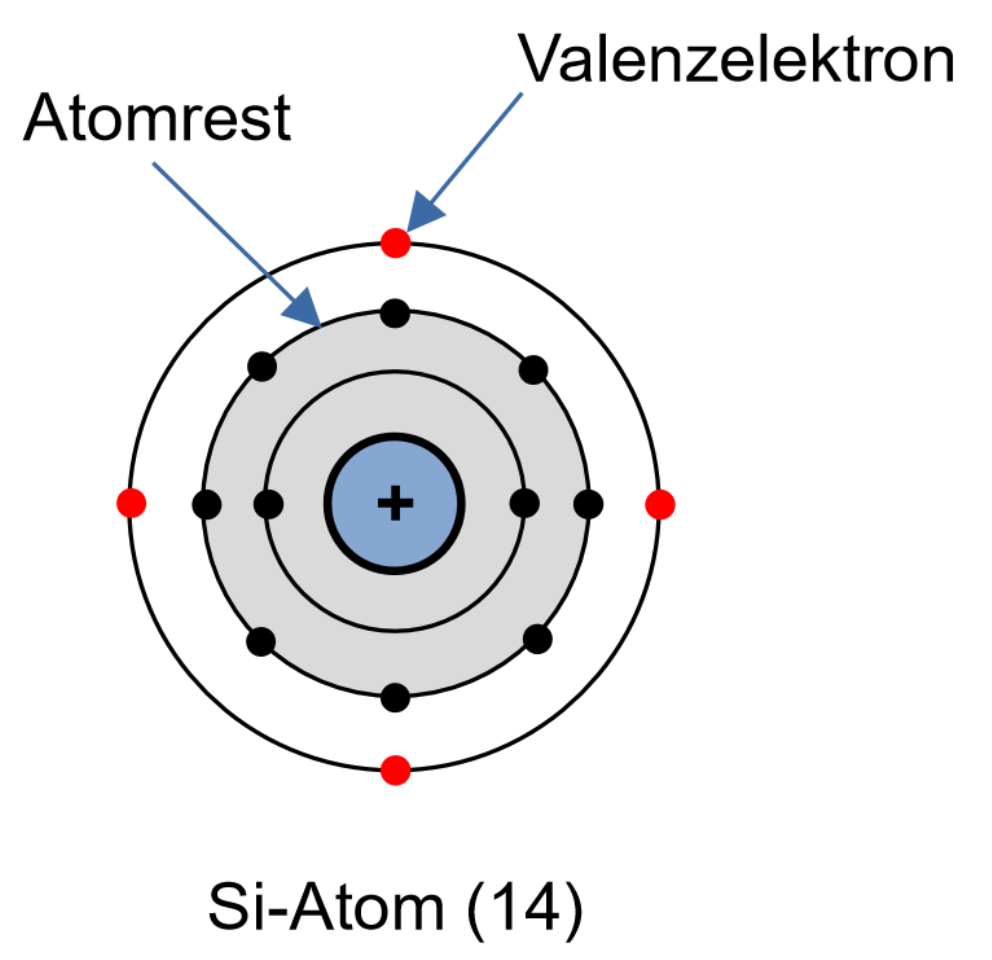
\includegraphics[width=\linewidth]{images/Si-Atom14}  
        \end{wrapfigure}
    Durch die thermische Bewegung der Atomem um ihre Ruhelage im Kristallgitter ist es möglich einige \textbf{Elektronenpaarbindungen} aufzubrechen.\newline
    Auf diese weise ein gelöstes Elektron bewegt sich im Kristallgitter frei und hinterlässt eine \textbf{positiv geladene Lücke im Kristallgitter} (Defektelektron)
\end{minipage}
\newline
\hspace{2cm}
\begin{minipage}{0.3\linewidth}
    \hspace{2cm}
    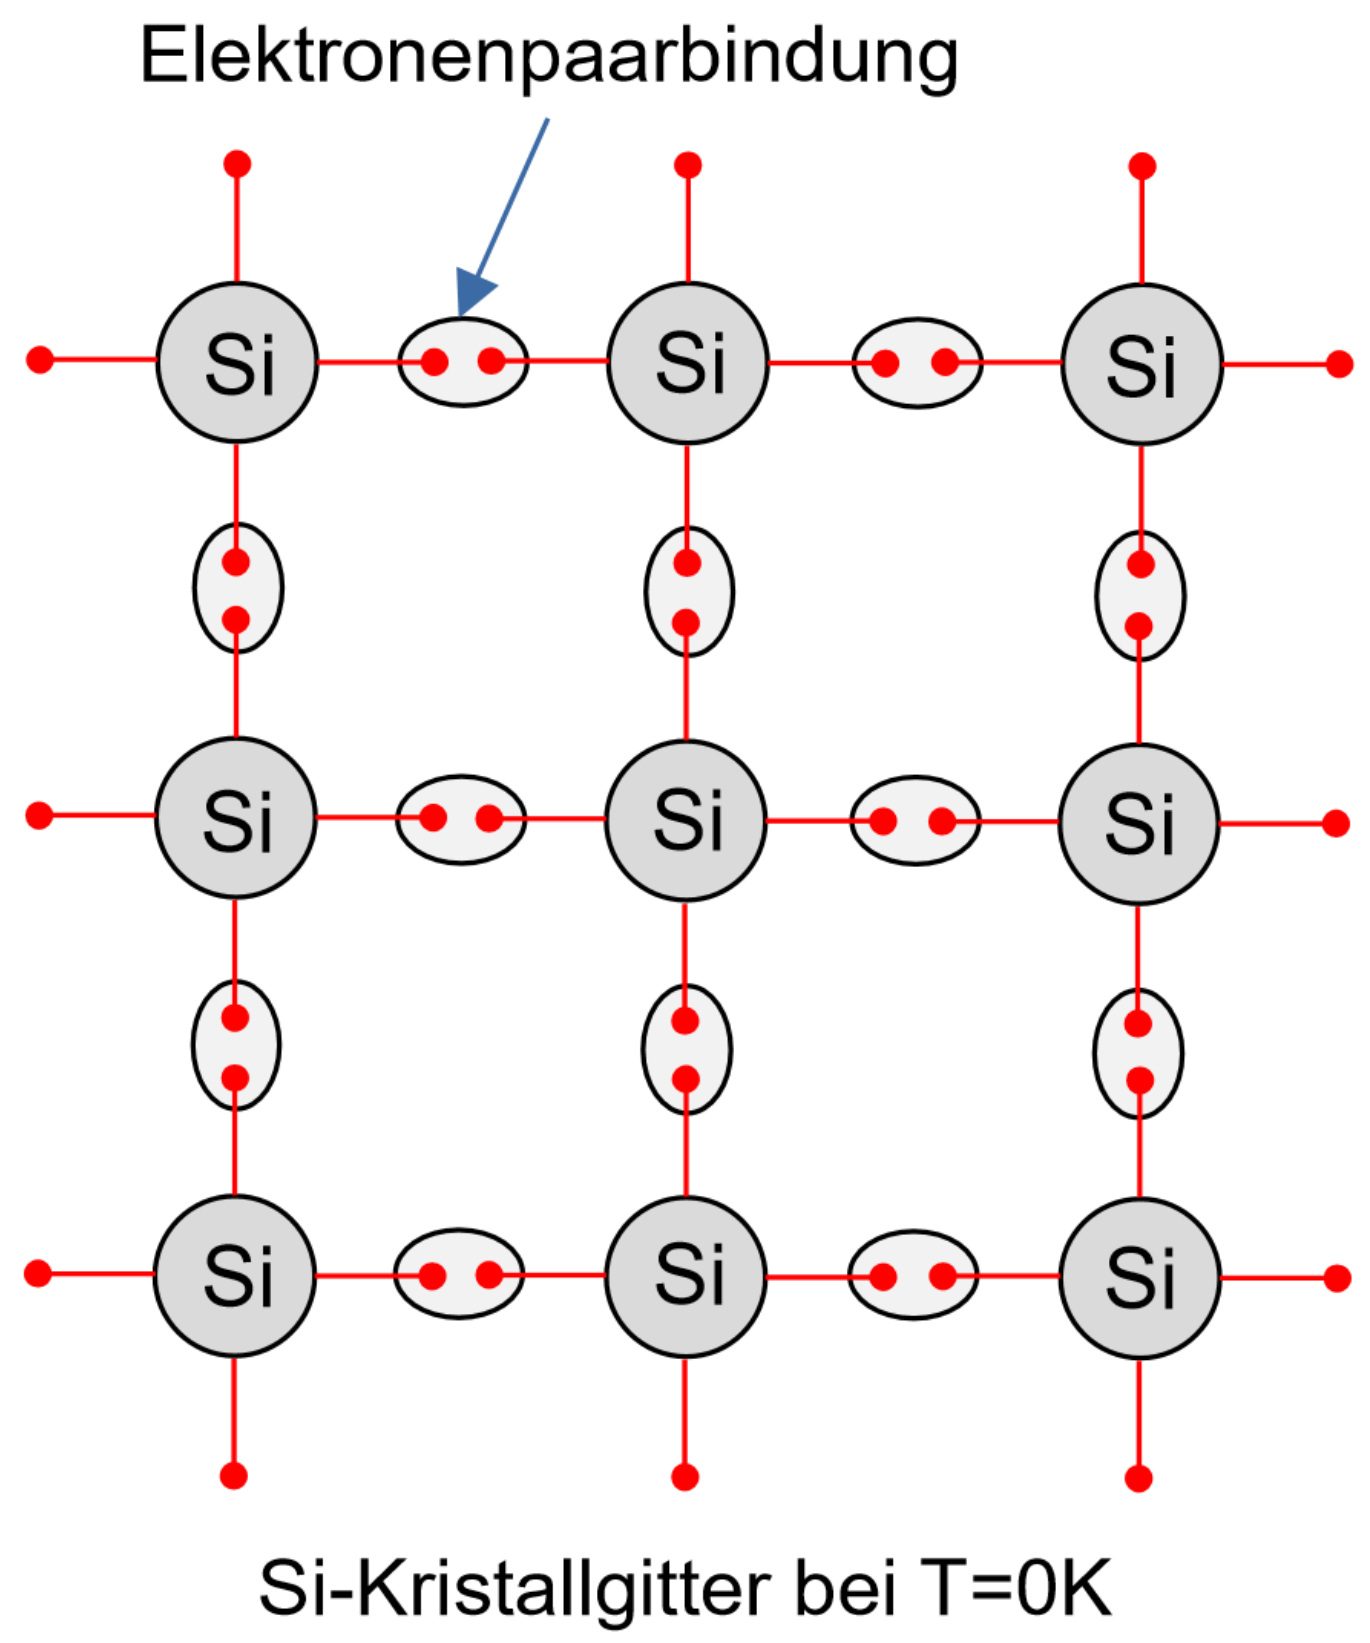
\includegraphics[width=0.8\linewidth]{images/RGSiT0K}
\end{minipage}
\hspace{2cm}
\begin{minipage}{0.3\linewidth}
    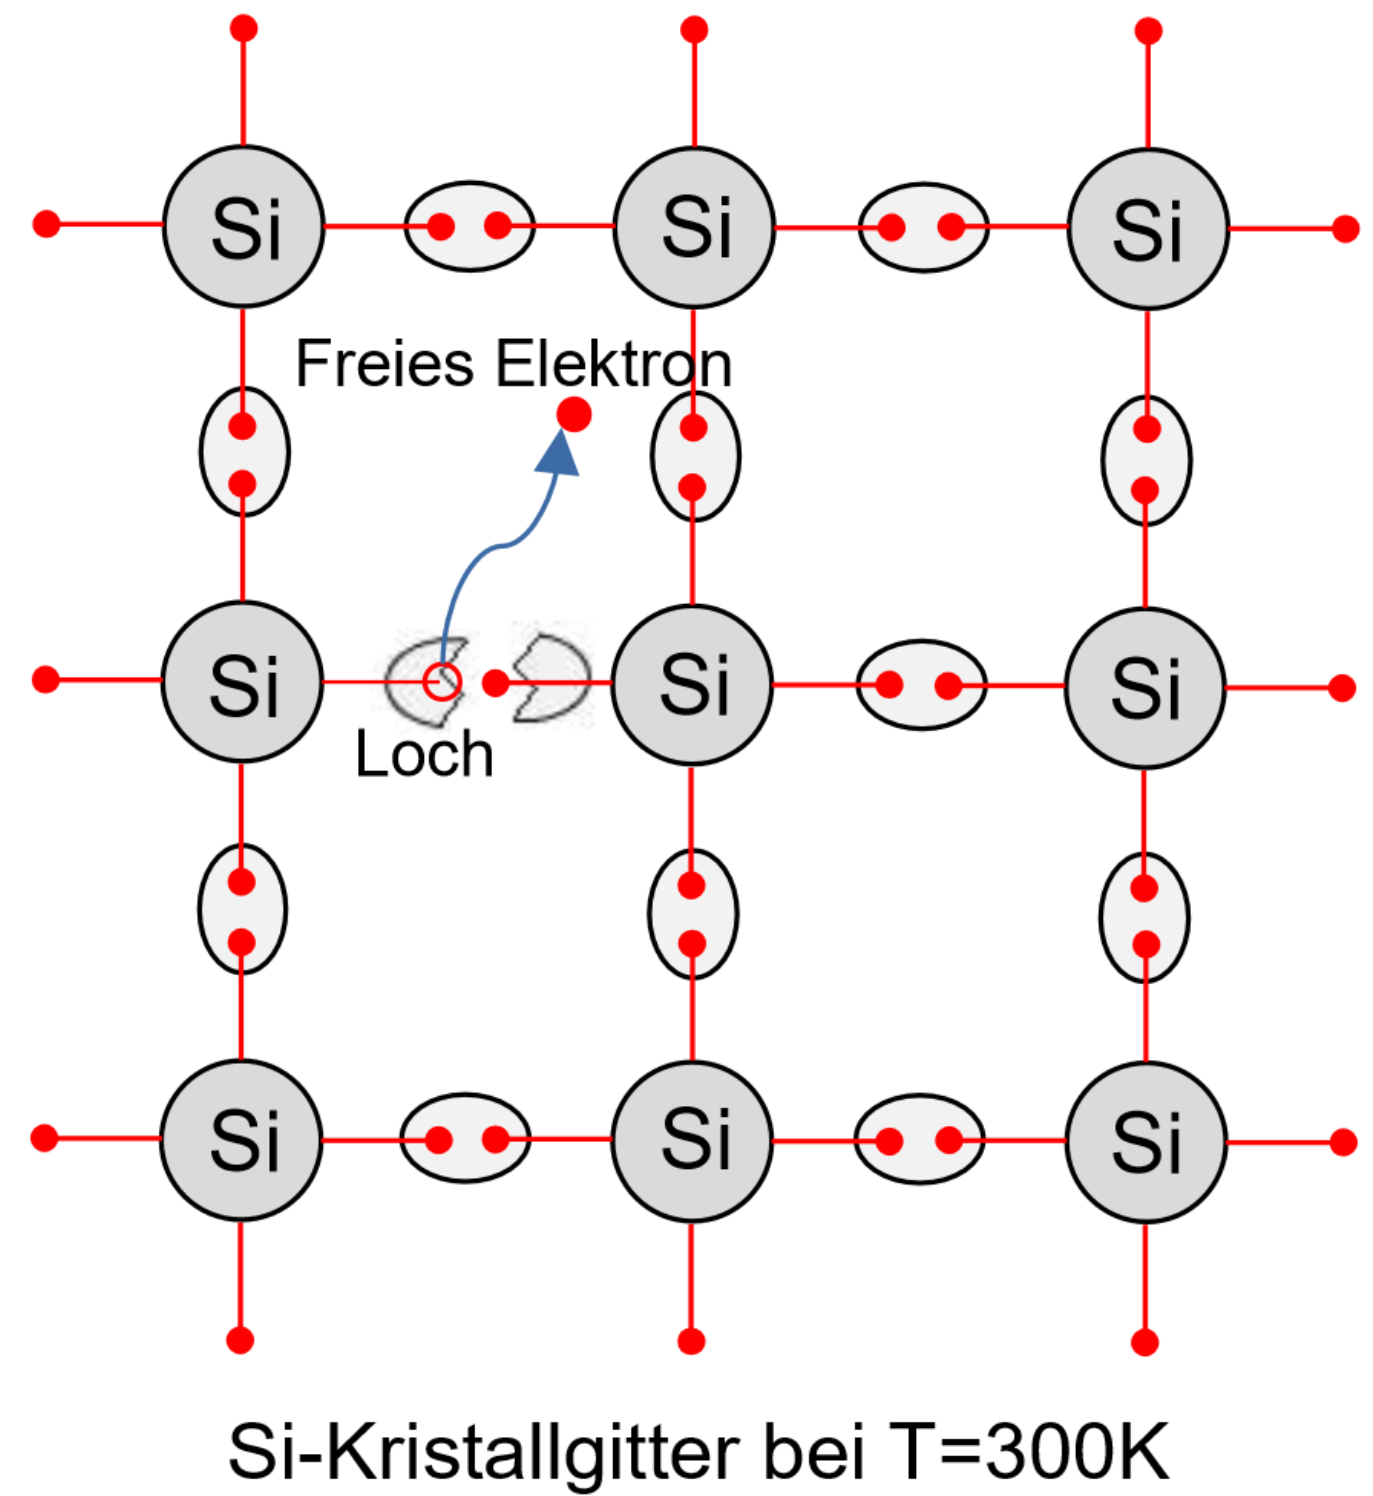
\includegraphics[width=0.8\linewidth]{images/RGSiT300K} 
\end{minipage}
    
\begin{multicols}{2}
\begin{minipage}{\linewidth}
    \subsection{Dotierung}
   Durch eine Dotierung des Halbleitermaterials mit Fremdatomen ist es möglich die Ladungsträgerdichte effizient zu kontrollieren:
\end{minipage}
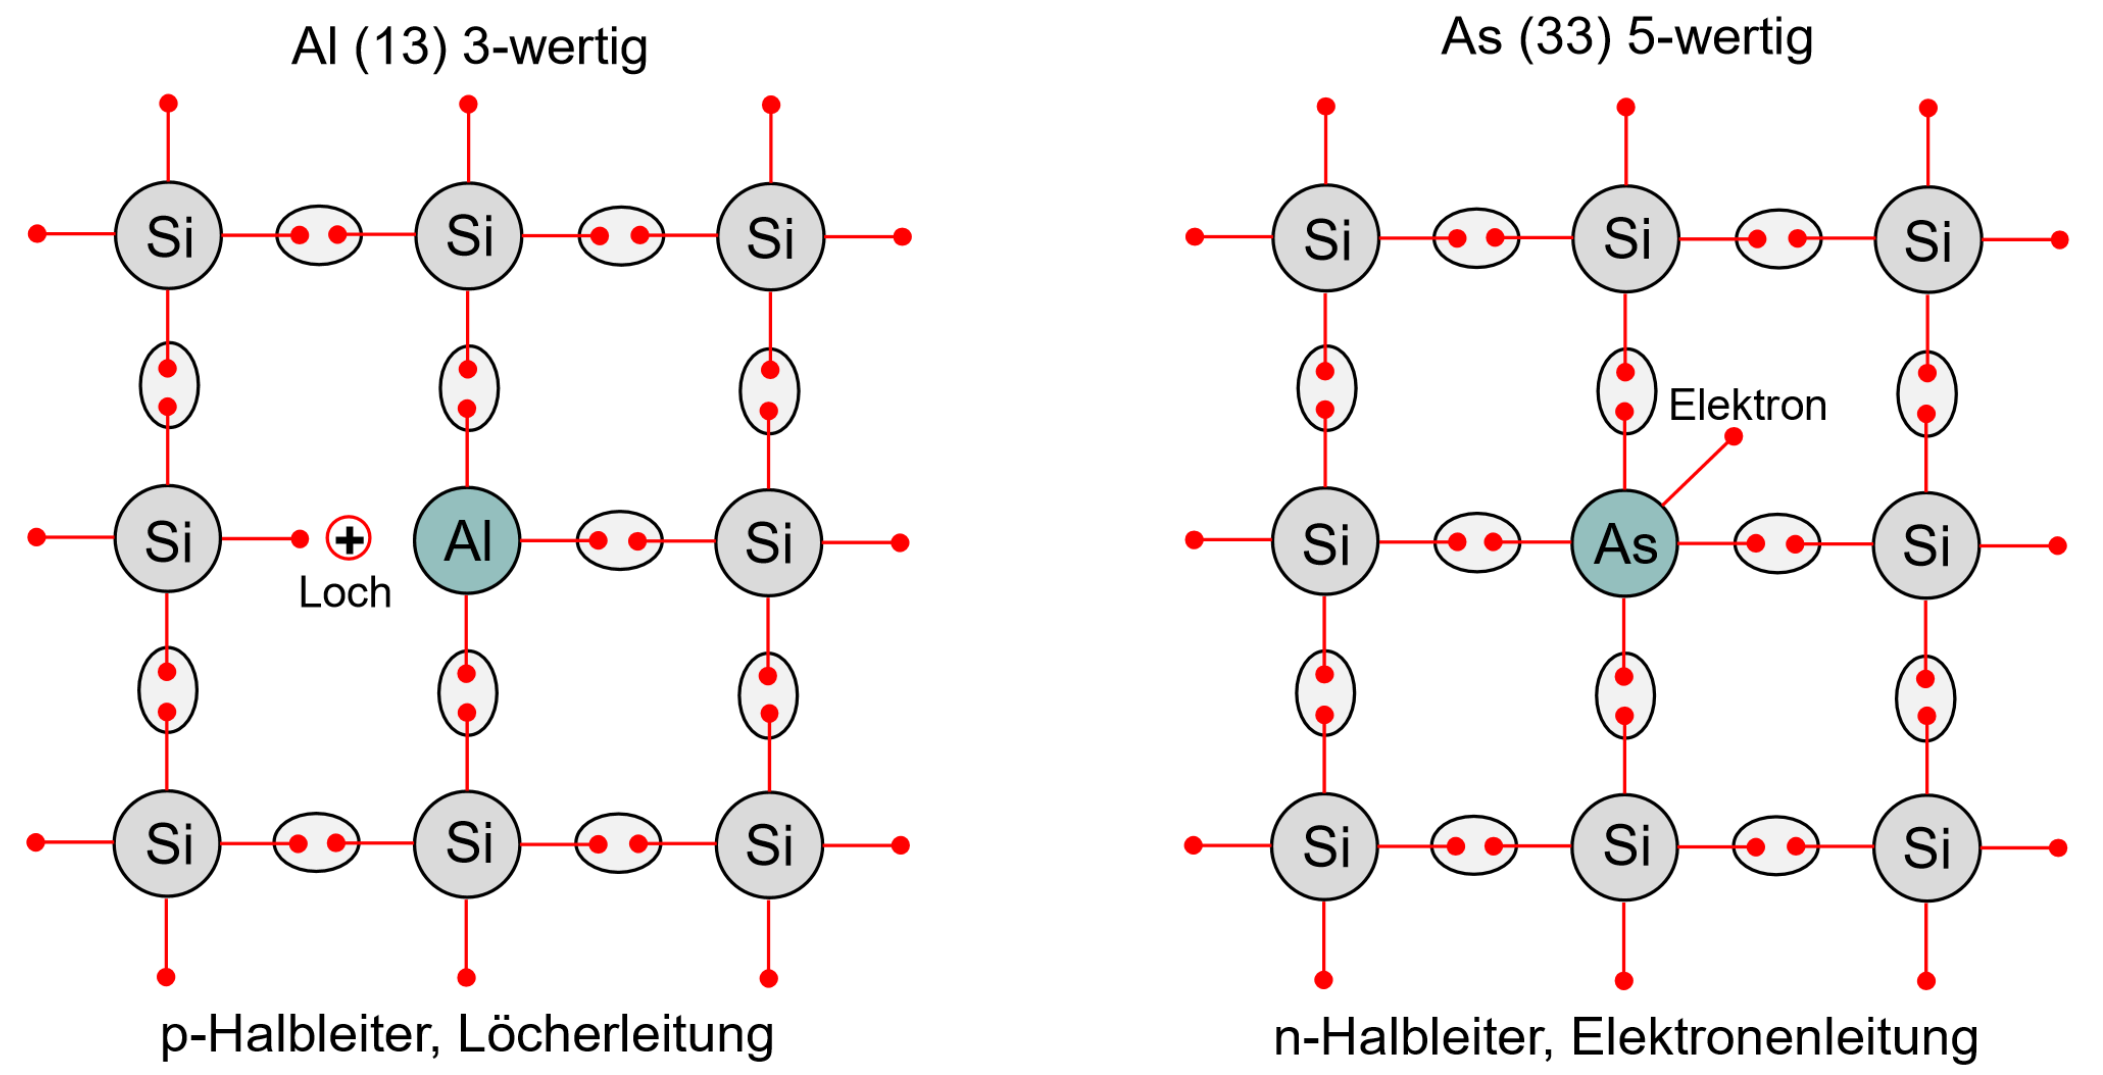
\includegraphics[width=0.8\linewidth]{images/SiAsDotierung}
\end{multicols}

\begin{multicols}{2}
    \begin{minipage}{\linewidth}
        \vspace{-2cm}
        \subsection{pn-Übergang}
        \subsubsection{Diffusionsstrom}
            Der Diffusionsstrom wird durch den Ladungsträgeraustausch zwischen beiden Halbleitergebieten erzeugt und dadurch verschwinden in der Grenzschicht alle freien Ladungsträger.\\
            Durch die Elektronenwanderung entsteht im n-Teil des Grenzgebiets die \textbf{ortsfeste} Positive Ladung(+). Die eindiffundierten Elektronen erzeugen im p-Teil des Grenzgebiets die \textbf{ortsfeste} negative Ladung (-). Die ortsfesten Ladungen erzeugen das elektrische Feld in der Raumladungszone und dammit auch den Driftstrom.\newline
            Der Driftstrom ist gegen den Diffusionsstrom gerichtet. Sobald die Ströme gleich sind, ist eine stabile Raumladungszone etabliert.   
    \end{minipage}
    
    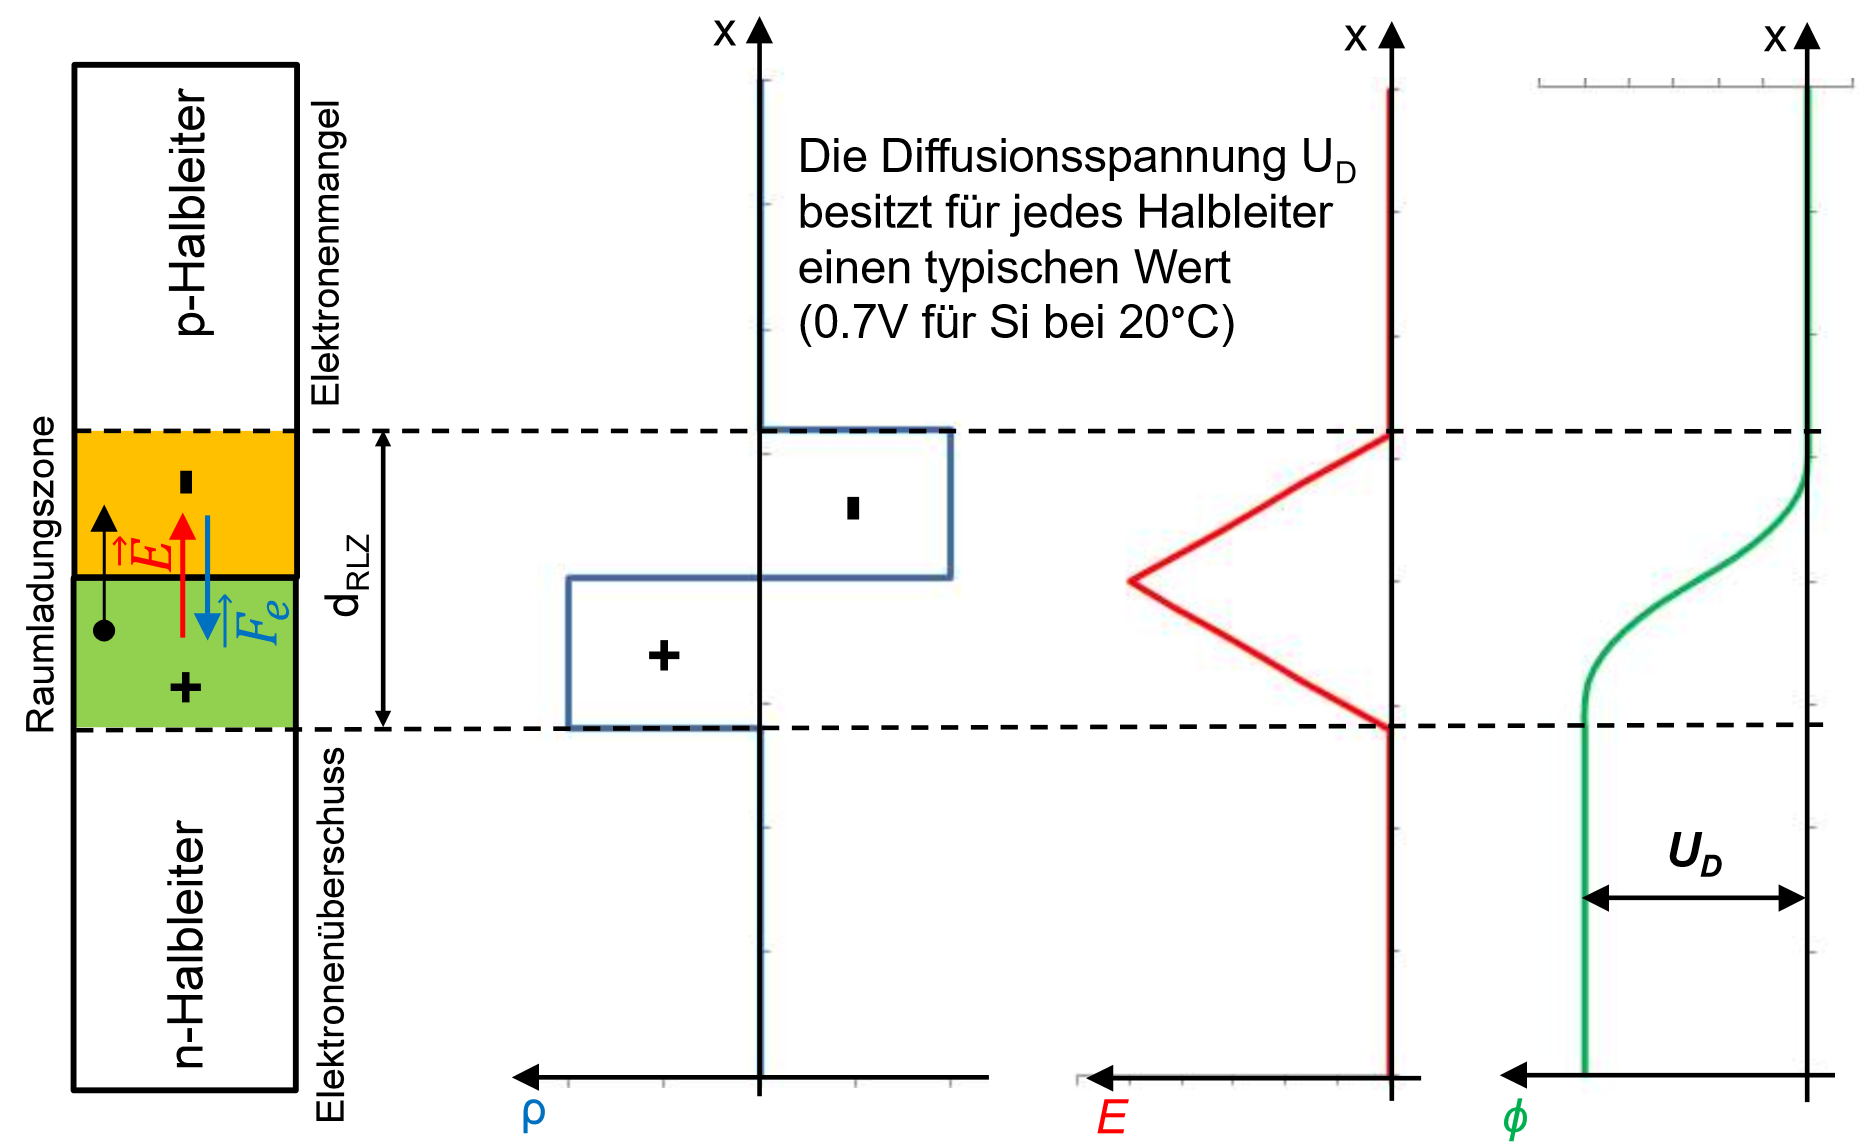
\includegraphics[width=0.9\linewidth]{images/pnuebergang}
\end{multicols}

\begin{minipage}{\linewidth}
        \subsubsection{pn-Übergang mit äusserer Spannung}
    \begin{wrapfigure}{r}{5cm}
       \vspace{-1cm}
        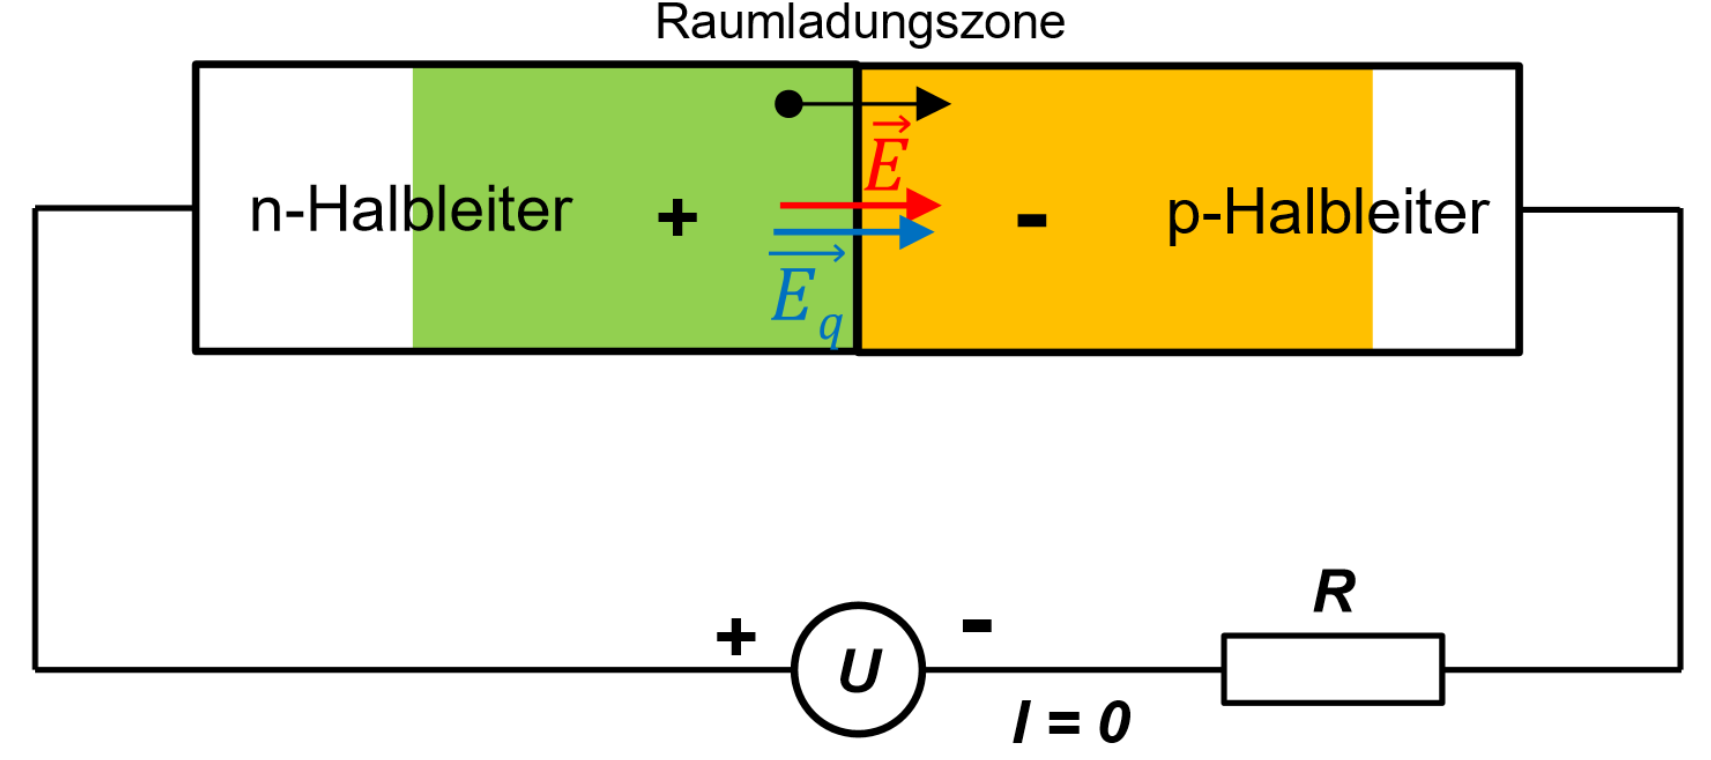
\includegraphics[width=\linewidth]{images/pnuebergengmitu}
    \end{wrapfigure}
    Die Spannungsquelle ist an den pn-Übergang in \textbf{Sperrrichtung} geschalten.\newline
    Die Spannung U vergrössert die Breite der Raumladungszone. Der Strom kann nicht über den pn-Übergang fliessen.
\end{minipage}
%TODO übersicht silizium germanium selen vor und nachteile
\clearpage
\section{Diode}
Eine Diode besteht aus pn-Übergängen und ist deswegen ein nichtlineares Element:
\begin{multicols}{2}
     \begin{minipage}{\linewidth}
         \begin{tabular}{ll}
             $ U_{DBR} $    & Durchbruchspanung  \\ 
             $ U_D $        & Diffusionsspannung (0.7V, Si)  \\ 
             $ U_F $        & Flussspannung \\ 
             $ U_R $        & Sperrspannung  \\ 
              $ i_F $       & Diffusionsstrom, Strom in Durchlassrichtung  \\ 
              $ i_R $       & Leckstrom, Strom in Sperrichtung \\ 
            \end{tabular} 
        \end{minipage}
        
         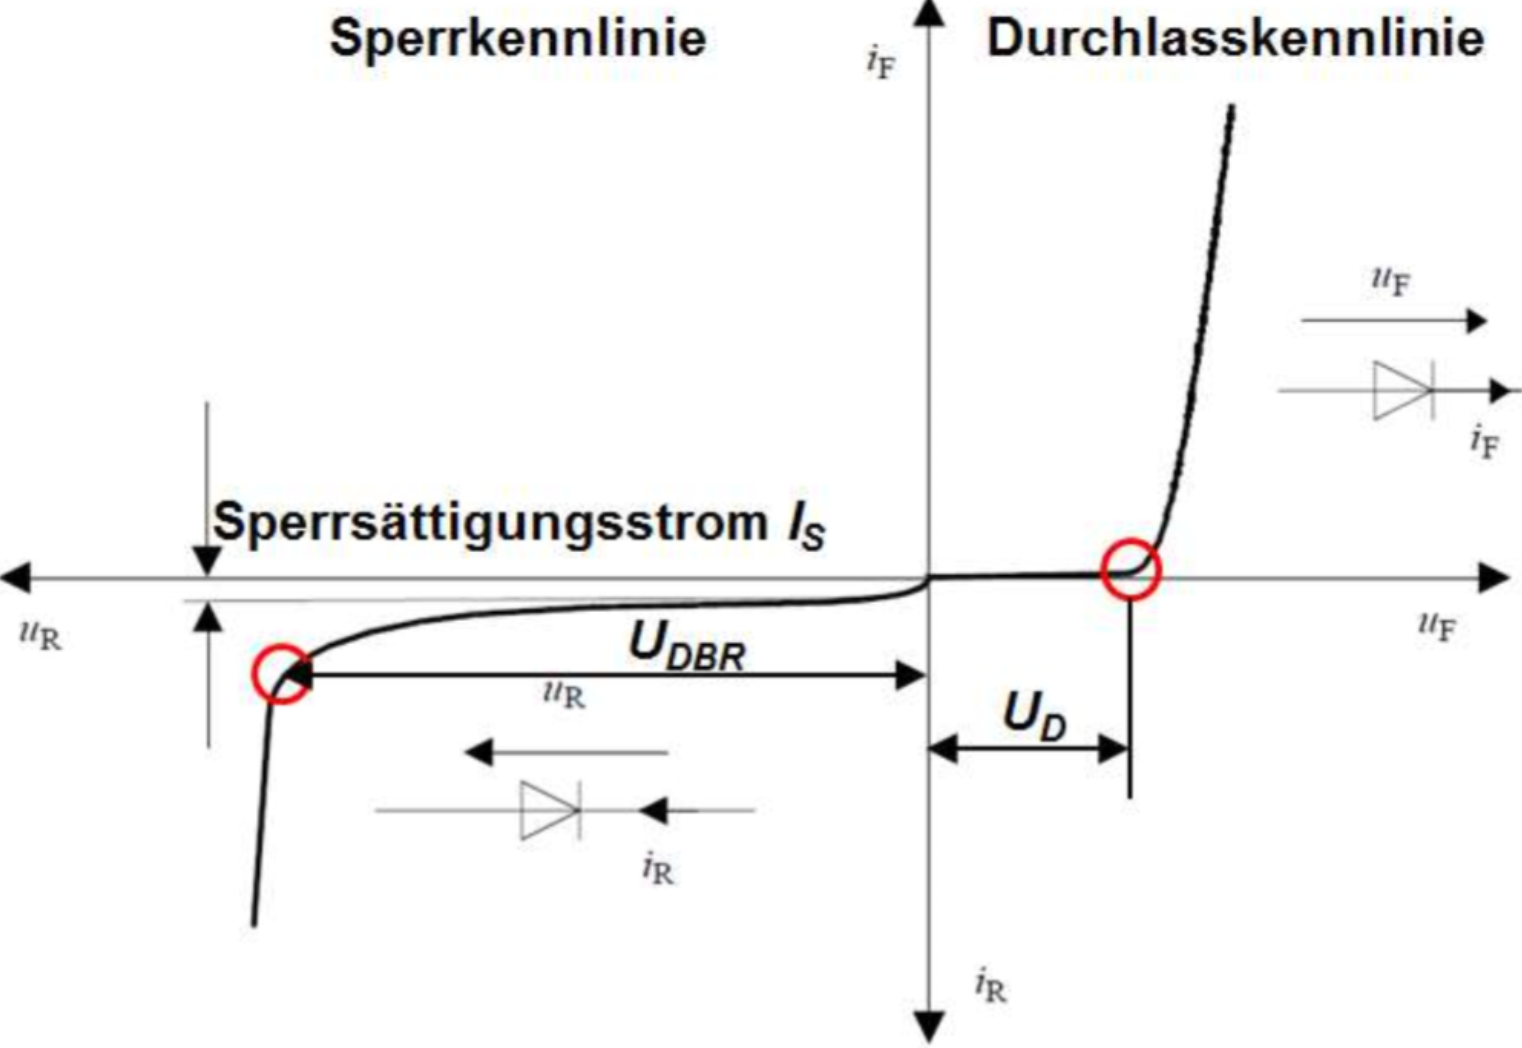
\includegraphics[width=0.8\linewidth]{images/kennlinieDiode}
\end{multicols}
\vspace{-1.5cm}
\begin{multicols}{2}
     \begin{minipage}{\linewidth}
         \begin{tabular}{ll}
             $ i_F ,\; u_F $& Durchlassrichtung\\
             $ U_{T0} $& Schwellenspannung\\
             $ r_F= \dfrac{\diff u_F}{\diff i_F} $& Differenzieller Durchlasswiderstand\\
            \end{tabular}       
    \end{minipage}
        
        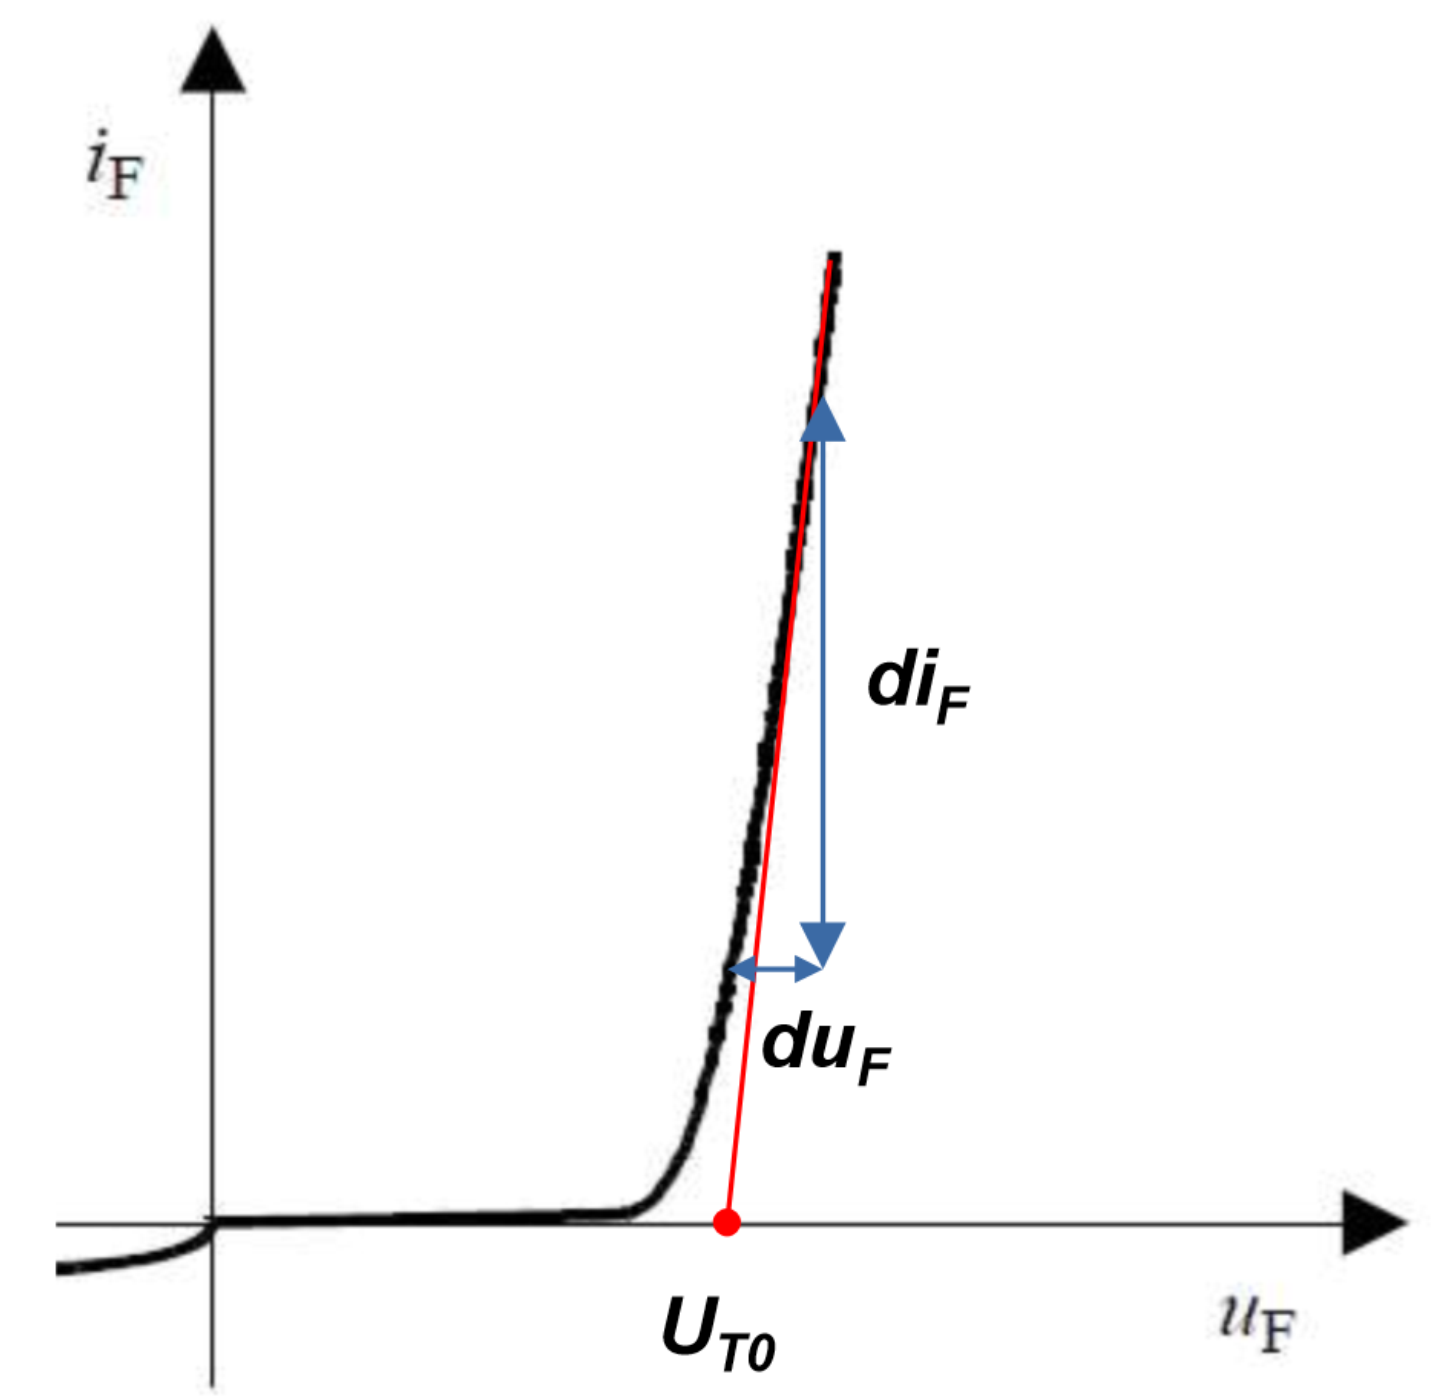
\includegraphics[width=0.4\linewidth]{images/dDiodeKennlinie}
\end{multicols}
\vspace{-1.5cm}
\subsection{Ersatzschaltbild}
\begin{multicols}{4}
    \begin{minipage}{\linewidth}
        \textbf{Reale Diode} \raggedright \newline\newline
        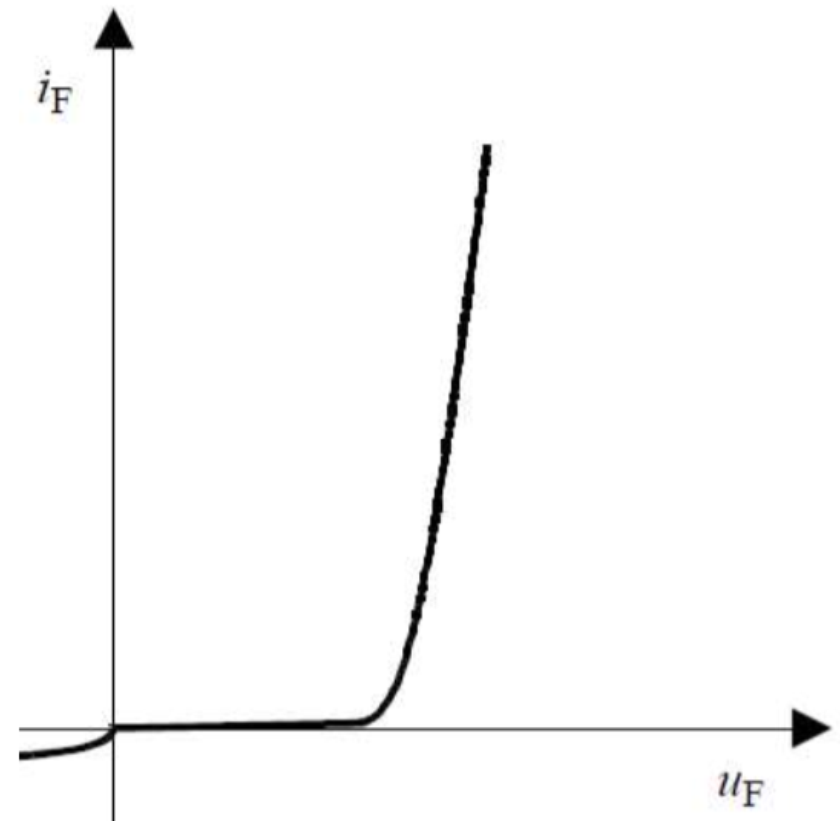
\includegraphics[width=0.7\linewidth]{images/realeDiode}
    \end{minipage}
    
    \begin{minipage}{\linewidth}
        \textbf{Ideale Diode ($ D_1 $)} \raggedright \newline\newline
        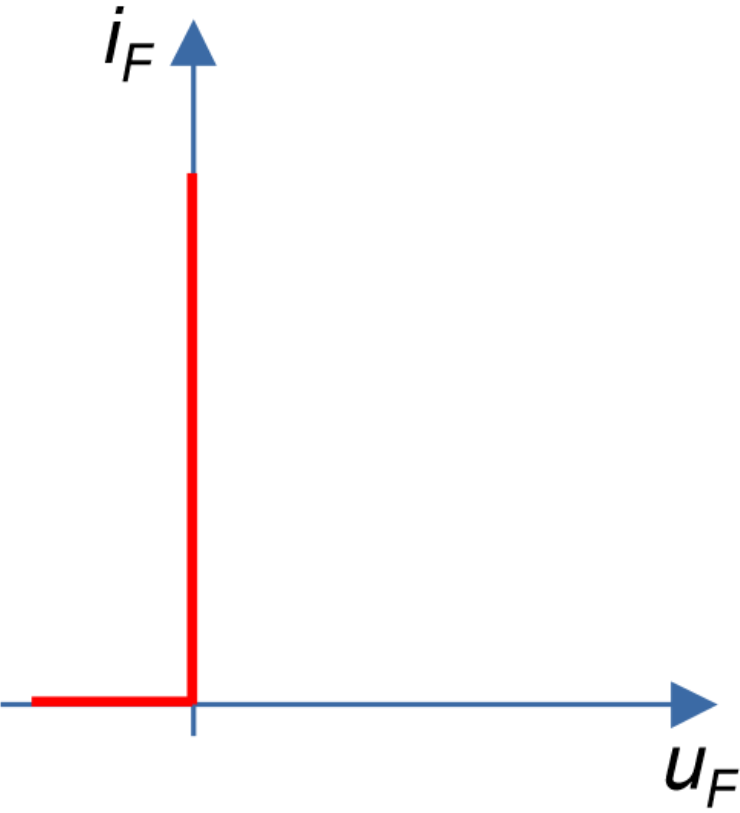
\includegraphics[width=0.7\linewidth]{images/idealeDiode}
    \end{minipage}
    
    \begin{minipage}{\linewidth}
        \textbf{Diode $ D_1 $ mit der Schwellenspannung ($  D_2 $)} \raggedright
        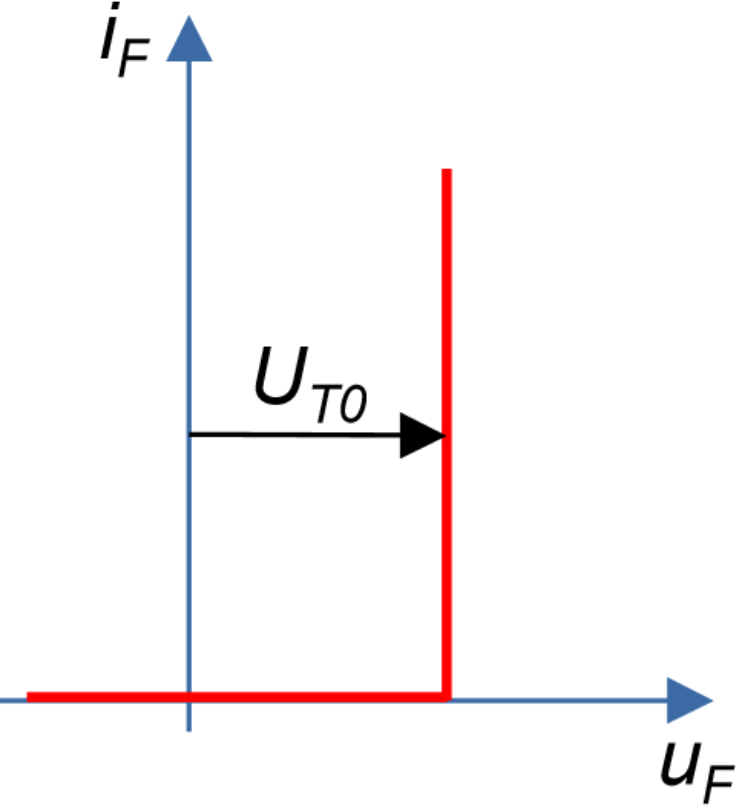
\includegraphics[width=0.6\linewidth]{images/idealeDiodeSP}
    \end{minipage}
    
    \begin{minipage}{\linewidth}
        \textbf{Diode $ D_2 $ mit dem Durchlasswiderstand ($ D_3 $)} \raggedright
        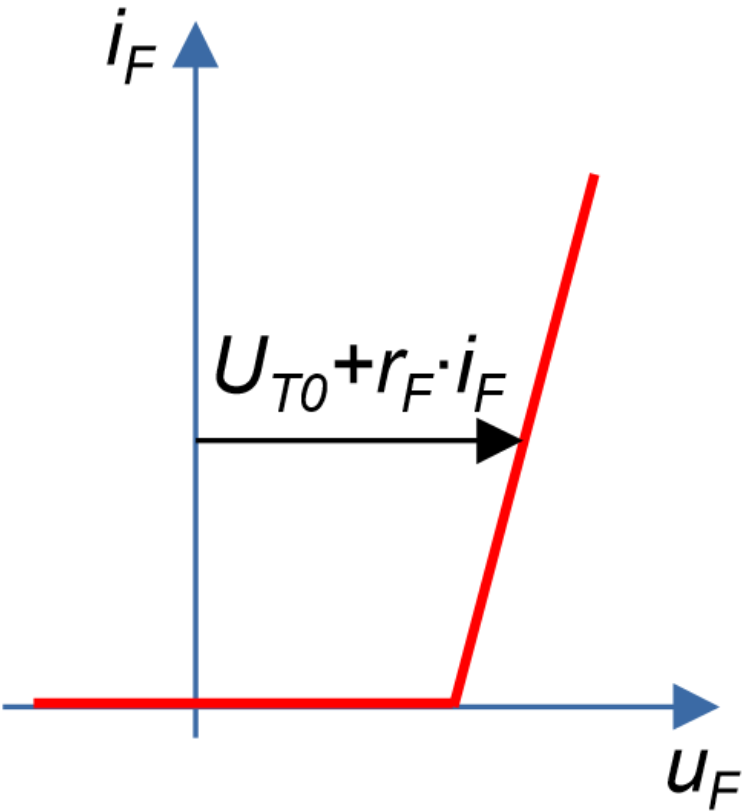
\includegraphics[width=0.6\linewidth]{images/idealeDiodeSPR}    
    \end{minipage}                       
\end{multicols}
\begin{multicols}{2}
\subsection{Grundformeln}
\begin{tabular}{ll}
    \textbf{Flussspannung}&\[ u_F = U_{T0} + i_F \cdot r_F \]\\[0.4cm]
    \textbf{Momentanleistung}&\[ p(t)=u_F(t)\cdot i_F(t) \]\\[0.4cm]
    \textbf{Verlustleistung}&\[ P_v= \frac{1}{T}\int_{0}^{T}\limits u_F(t)\cdot i_F(t)~dt = U_{T0}\cdot \int_{0}^{T}\limits i_F(t)~dt + r_F\cdot\frac{1}{T}\int_{0}^{T}\limits i^2_F(t)~dt = U_{T0}\cdot I_{FAV}+r_F\cdot I_{FRMS}^2 \]\\[0.2cm]
    $ I_{FAV}$ & \qquad arithmetische Mittelwert von $ i_F $\\
    $ I_{FRMS} $ & \qquad Effektivwert von $ i_F $\\    
\end{tabular}

\hspace{1cm}\vspace{-0.5cm}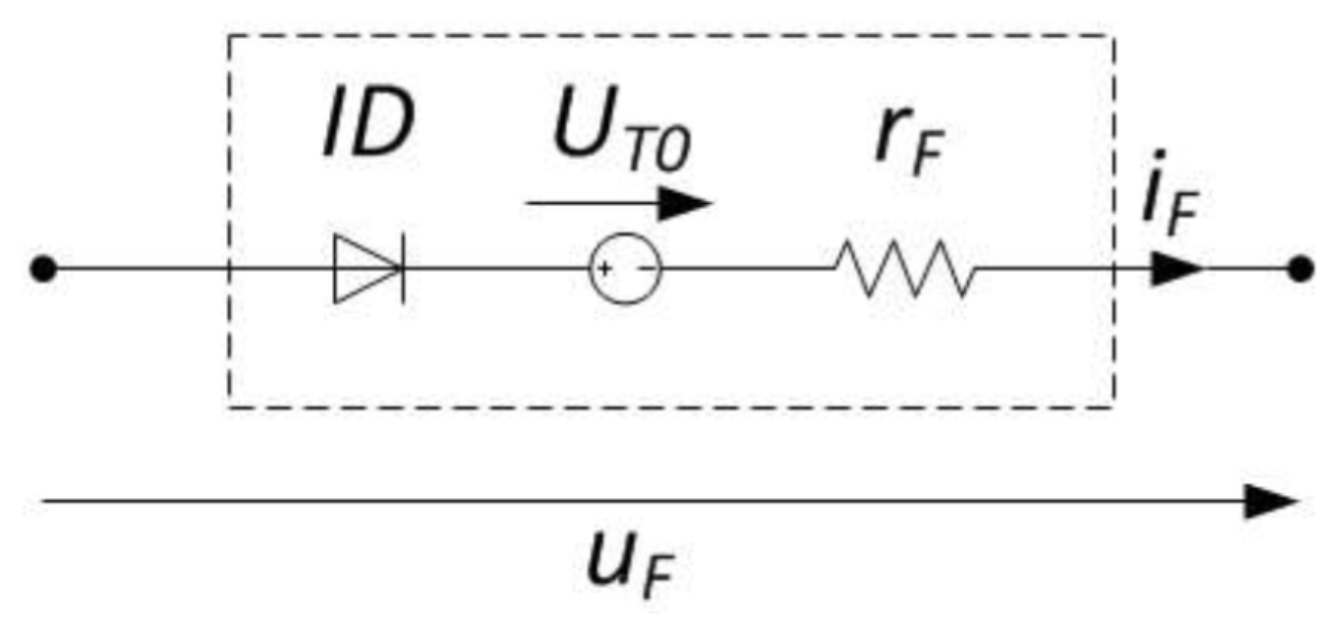
\includegraphics[width=0.6\linewidth]{images/ESBDiode} 
\end{multicols}

\subsection{Schaltverhalten und Schaltverluste}
    \begin{minipage}{0.7\linewidth}
        \raggedright
        \textbf{Durchlassverzug:}\newline
        freie Ladungsträger müssen zuerst die ladungsfreie Zone "füllen"\newline\newline
        \textbf{Sperrverzug}\newline
        freie Ladungsträge müssen zuerst das Gebiet des pn-Überganges freiräumen\newline\newline
        Diese Erscheinungen sind wichtig bei  $\nicefrac{\diff u}{\diff t} > 100 \nicefrac{V}{\mu s} \; und \; \nicefrac{\diff i}{\diff t} > 10 \nicefrac{A}{\mu s} $
        \begin{tabular}{ll}
            $ I_{RM} $&Maximalwert des Rückstromes\\
            $ U_{RM} $&Maximalwert der Rückspannung\\
        \end{tabular}
    \end{minipage}   
    \begin{minipage}{0.3\linewidth}
        \vspace{-0.8cm}
        \raggedleft
            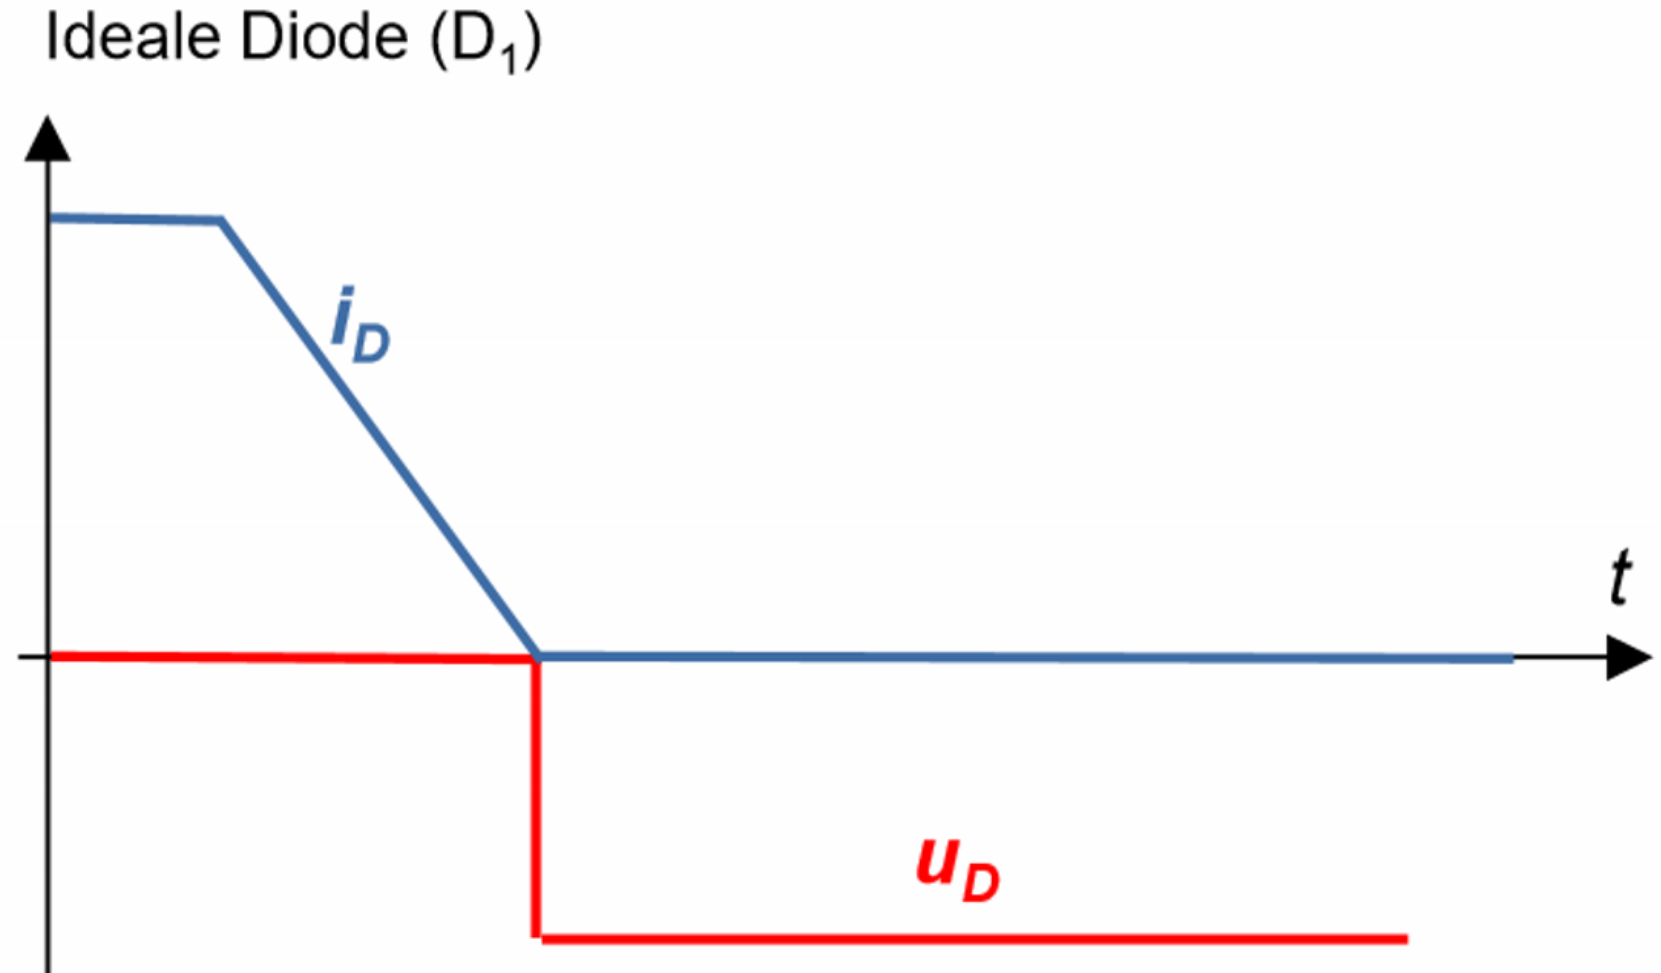
\includegraphics[width=\linewidth]{images/idealeDiodeSS}           
            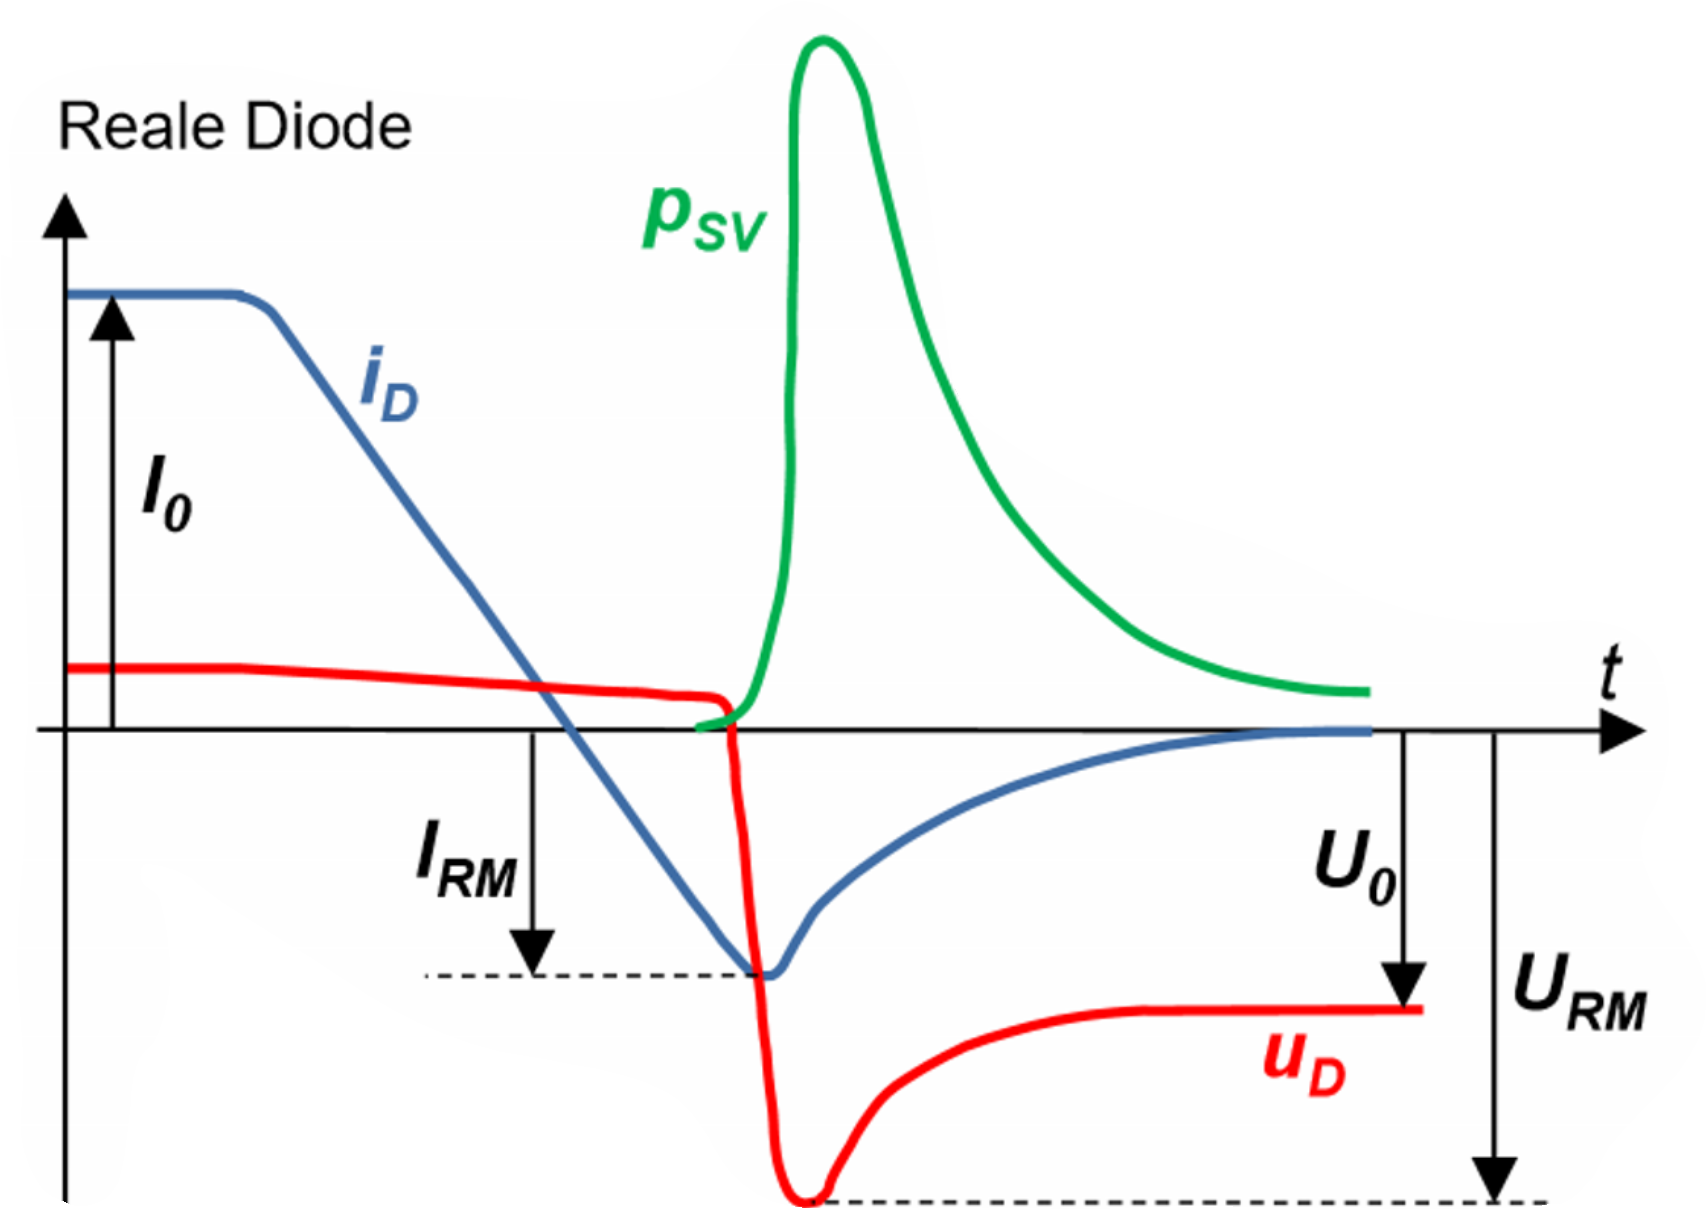
\includegraphics[width=\linewidth]{images/realeDiodeSS}
    \end{minipage}
\clearpage

\section{Transistor}
\vspace{-0.2cm}
\subsection{Bipolarer Transistor}
\vspace{-0.2cm}
\subsubsection{Wirkungsprinzip}
Ein Bipolartransistor besteht aus drei dünnen dotierten Halbleiterschichten, d.h. aus zwei pn-Übergängen. \newline Gemäss der Reihenfolge und dem Dotierungstyp der Schichtung werden Bipolartransistoren in npn- und pnp-Typen unterteilt.\newline Als Leistungstransistoren werden überwiegend npn-Transistoren in der Emitter-Schaltung verwendet\newline
\hspace*{2cm}
\begin{tabular}{ccc}
     \textbf{Wirkungsprinzip}&\textbf{Aufbau}&\textbf{Schaltzeichen}\\
     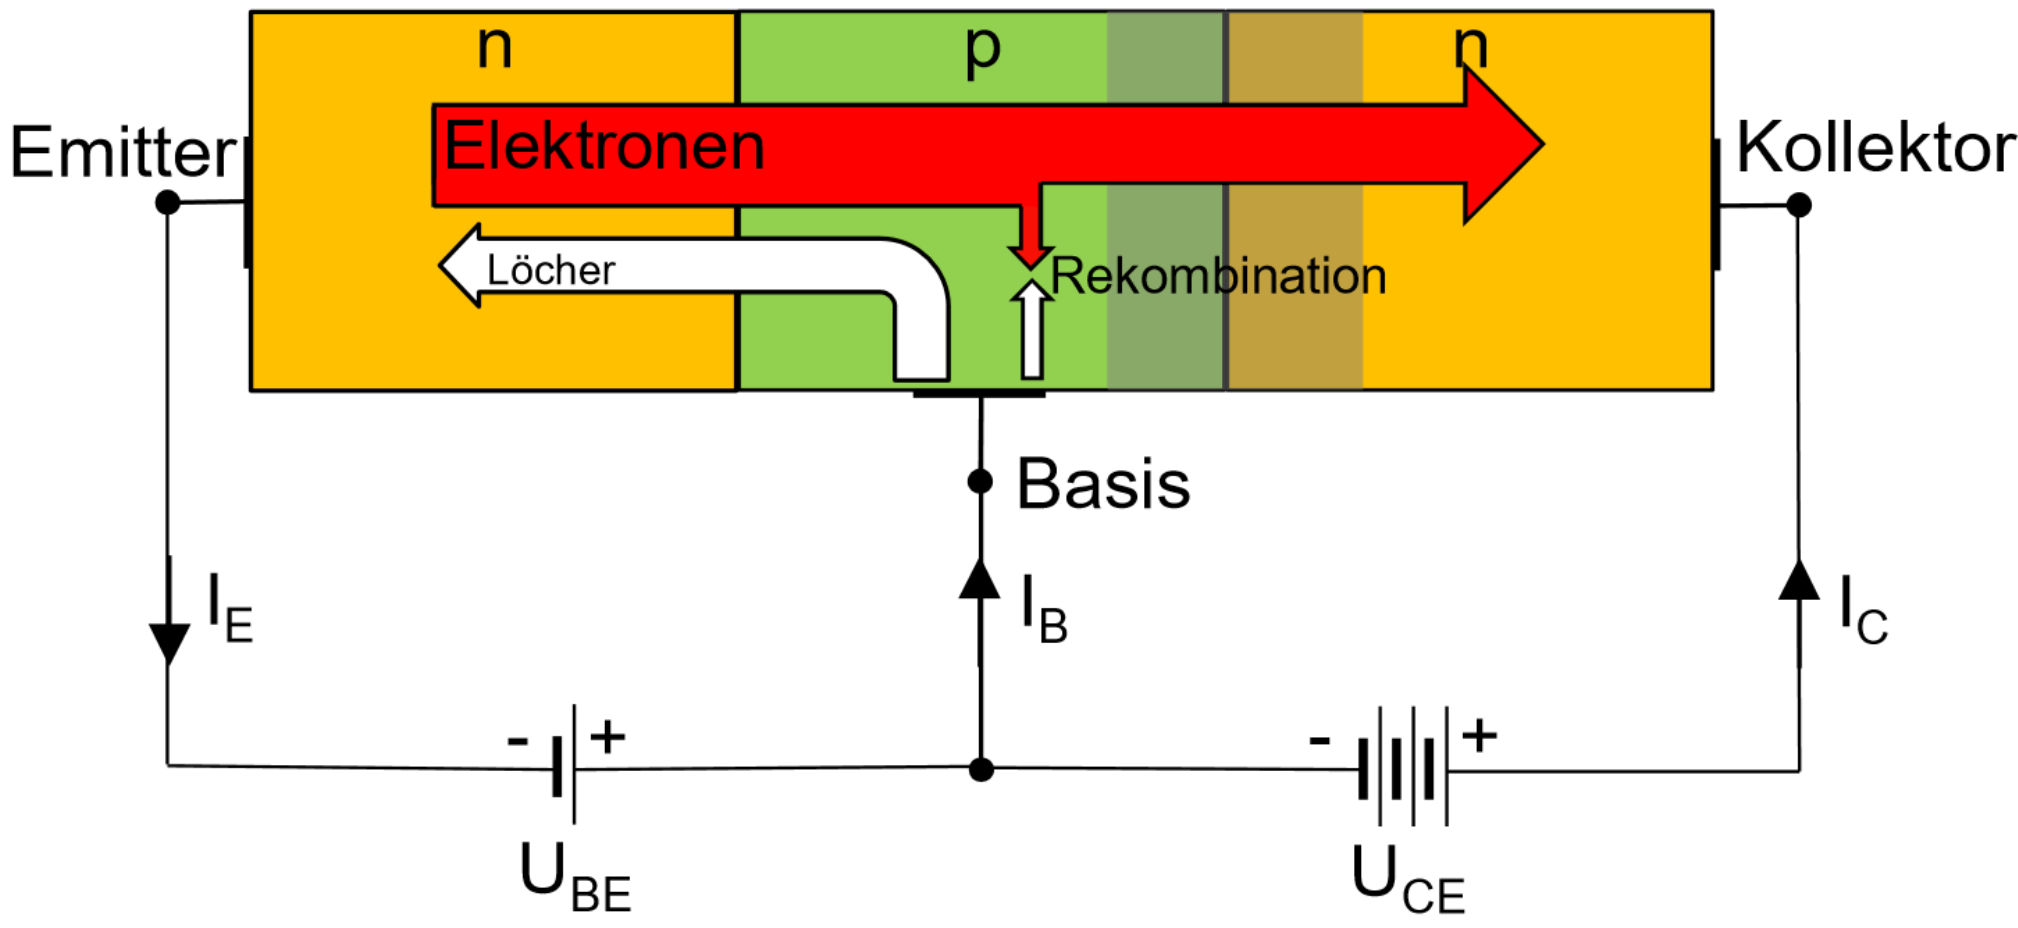
\includegraphics[width=0.35\linewidth]{images/npnTransistor}&
     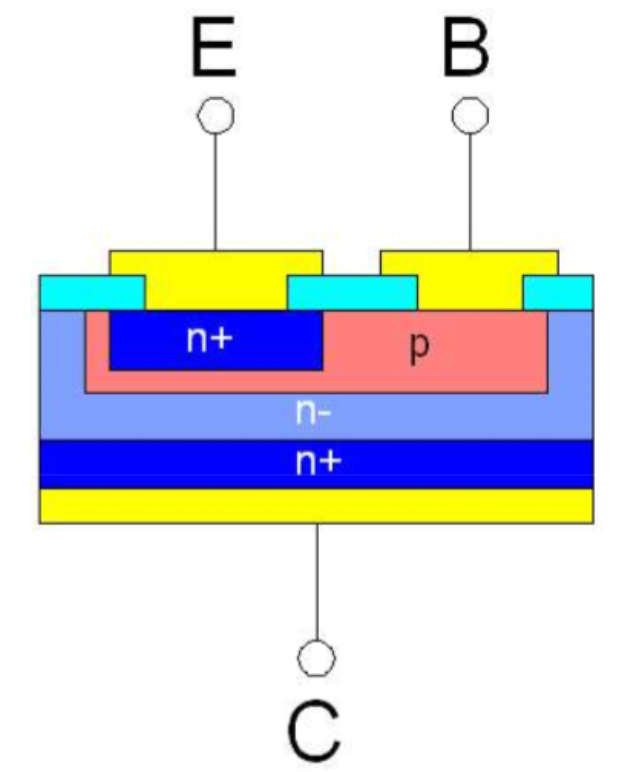
\includegraphics[width=0.15\linewidth]{images/aufbautransnpn}&
     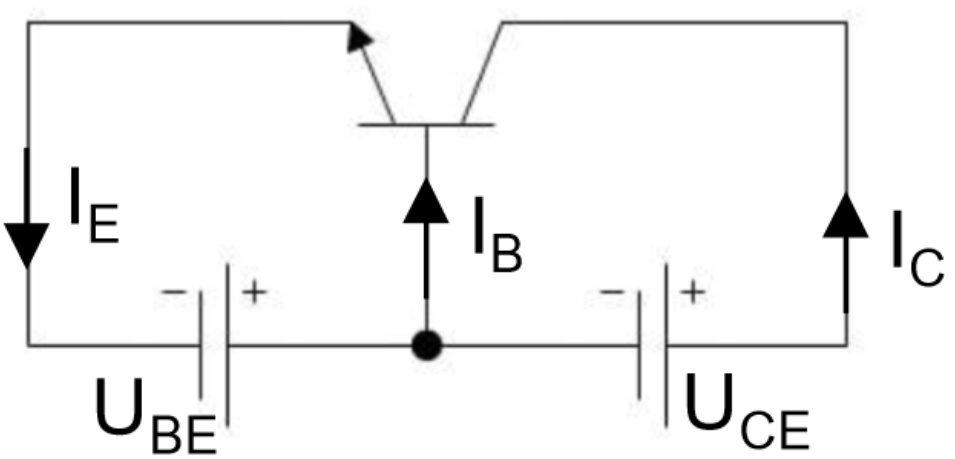
\includegraphics[width=0.25\linewidth]{images/esbtransnpn} \\
\end{tabular}

\subsubsection{Schaltverhalten}
\begin{minipage}{0.6\linewidth}
    \begin{wrapfigure}{r}{4cm}
        \includegraphics[width=\linewidth]{images/npnTransemitter}
    \end{wrapfigure}
    \raggedright
    \textbf{Im Sättigungsbreich} ist der Basisstrom so gross, dass sich in der Basiszone mehr Ladungsträger befinden als für den Kollektorstrom nötig ist.\newline\newline
    Die beiden pn-Übergänge sind in die Durchlassrichtung polarisiert.\newline
    $ U_{BE}>U_{CE} $ und $ U_{BC}>0 $\newline\newline
    Im Verstärkungsbereich gilt: $ \beta = \dfrac{I_C}{I_B} $\newline \newline
    \textbf{Im Schaltbetrieb} werden die Arbeitspunkte \textbf{I} (vorwärts sperrend) und \textbf{III} (Durchlassbetrieb -Sättigung) verwendet.
\end{minipage}
\begin{minipage}{0.4\linewidth}
    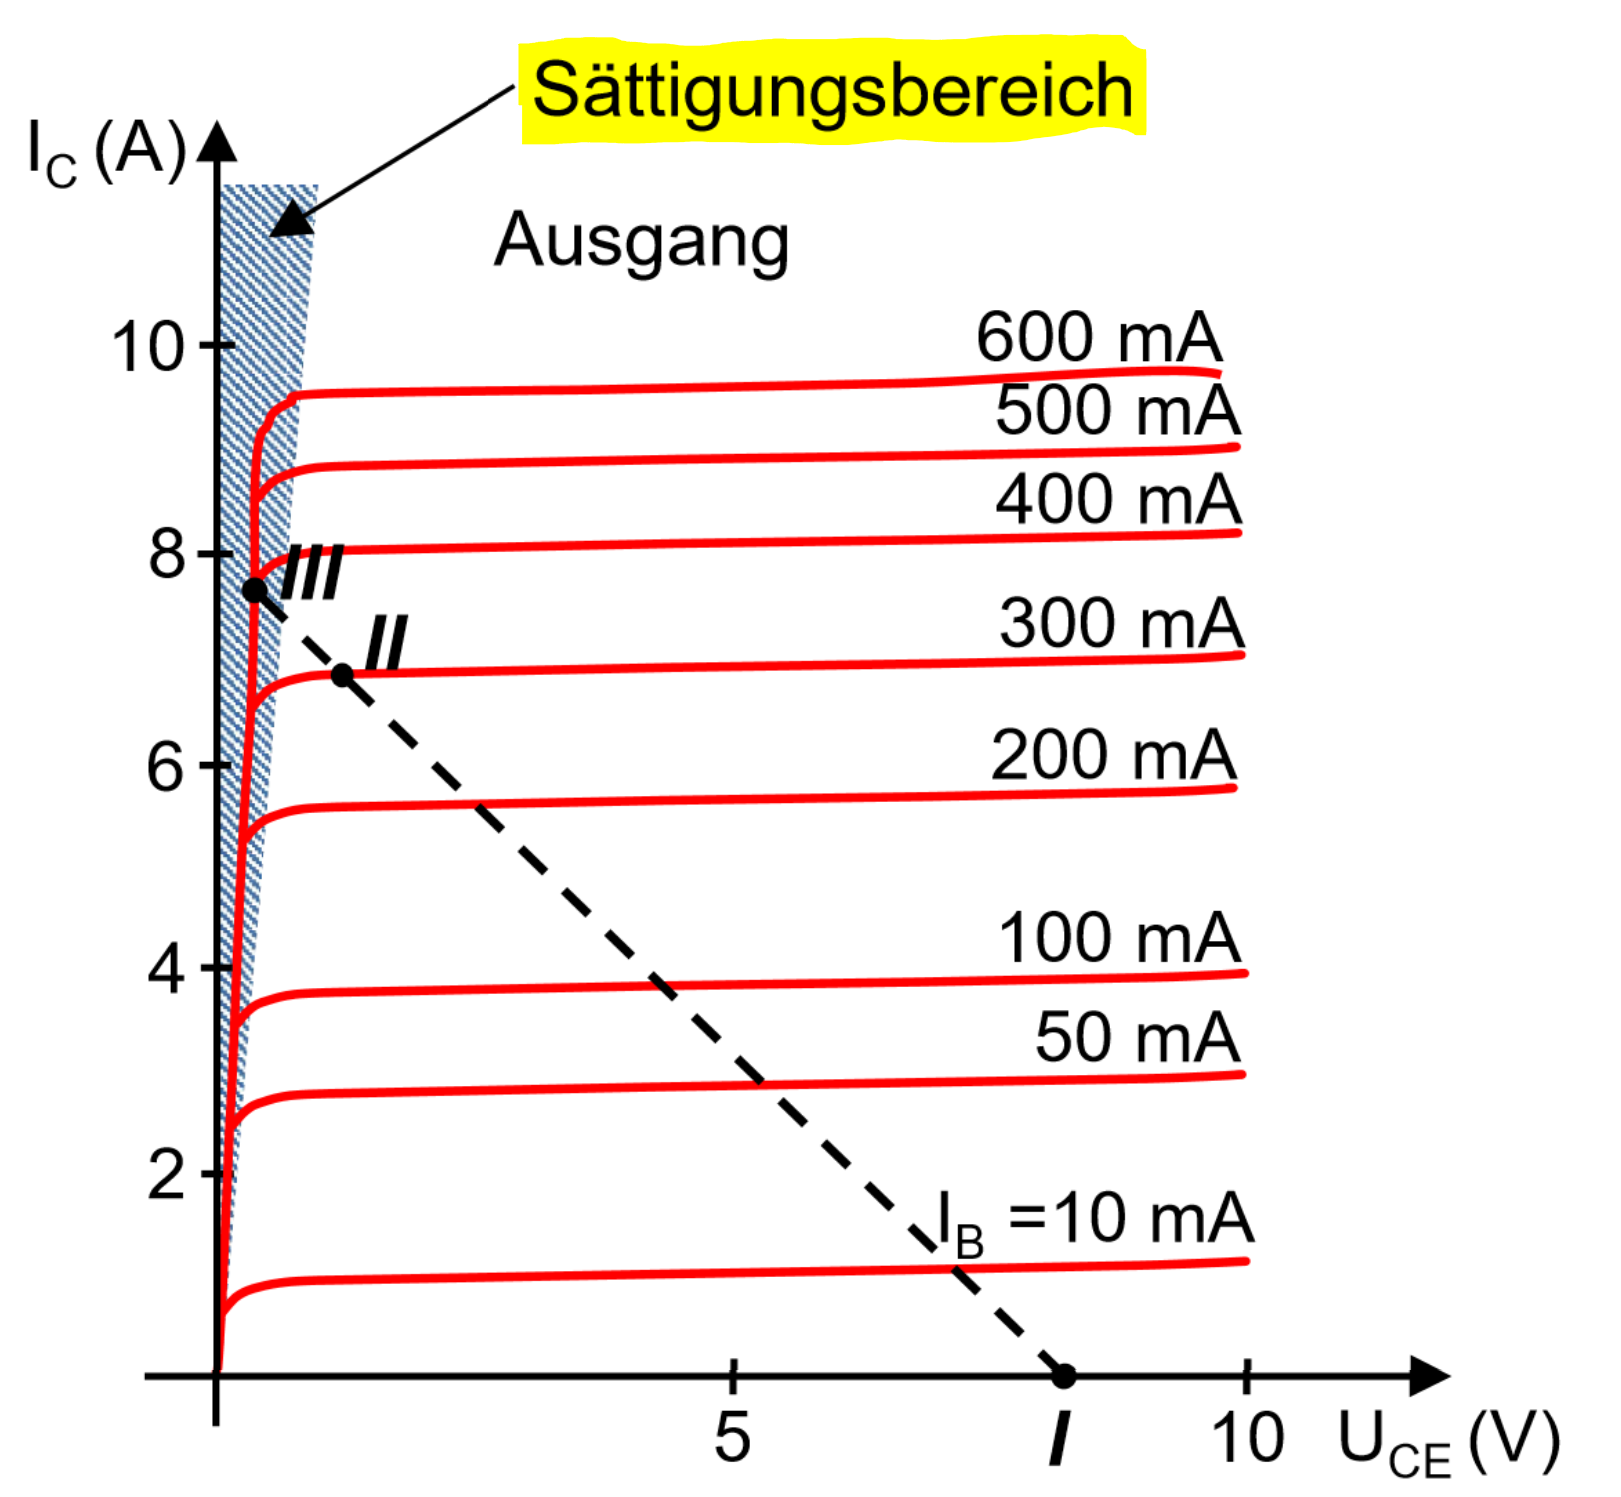
\includegraphics[width=0.8\linewidth]{images/npnTranskennlinie}
\end{minipage}
\subsubsection{Kennwerte}
\begin{minipage}{0.5\linewidth}
	\renewcommand{\arraystretch}{1.2}
\begin{tabular}{l p{7cm}} 
    \textbf{$ U_{CES} $}&\textbf{Kollektor-Emitter-Sperrspannung}\\
    &Der höchstzulässige Wert der $ U_{CES} $ bei Ansteuerung mit einer negativen $ U_{BE} $\\
    \textbf{$ U_{CE0} $}&\textbf{Kollektor-Emitter-Sperrspannung}\\%RICHTIG??
    & Der höchstzulässige Wert der $ U_{CE} $ bei offenem Basisanschluss\\
    \textbf{$ I_{CAVM} $}&\textbf{Kollektor-Dauergrenzstrom}\\
    &\mbox{Der höchstzulässige Wert des Gleichstrom-} \mbox{Mittelwerts bei vorgegebener Temperatur}\\
    \textbf{$ I_{CRM} $}&\textbf{periodischer Kollektor-Spitzenstrom}\\
    &\mbox{Der höchstzulässige Wert eines Pulsstromes} \mbox{mit angegebener Periodendauer und Einschaltdauer}\\
\end{tabular}
\end{minipage}
\begin{minipage}{0.5\linewidth}
    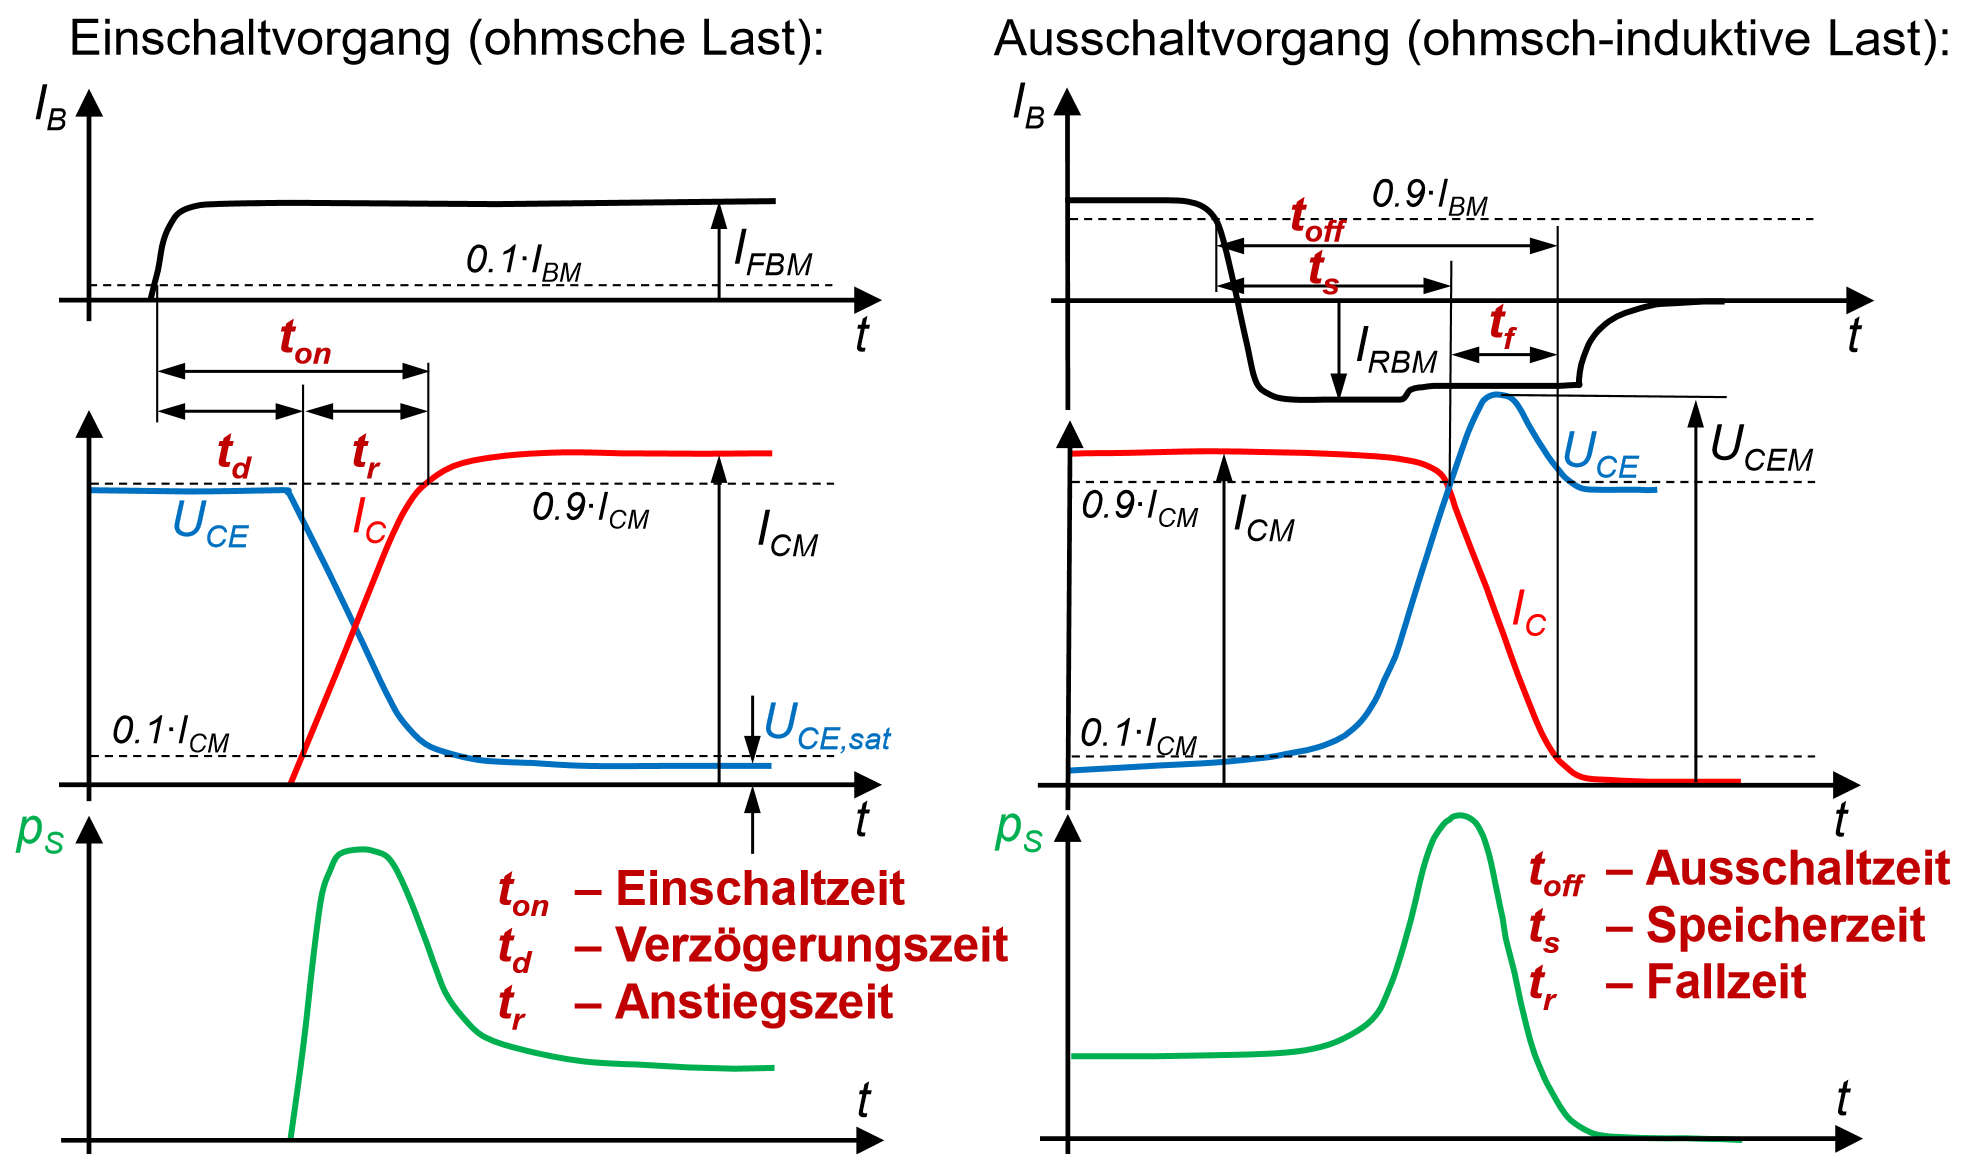
\includegraphics[width=\linewidth]{images/npnTransESV}
\end{minipage}

\begin{minipage}{0.5\linewidth}
    \subsubsection{Verluste}
    \begin{itemize}
        \item Einschaltverluste
        \item Ausschaltverluste
        \item Durchlassverluste
        \item Sperrverluste
    \end{itemize}
\end{minipage}
\begin{minipage}{0.5\linewidth}
    \hspace{0.5cm}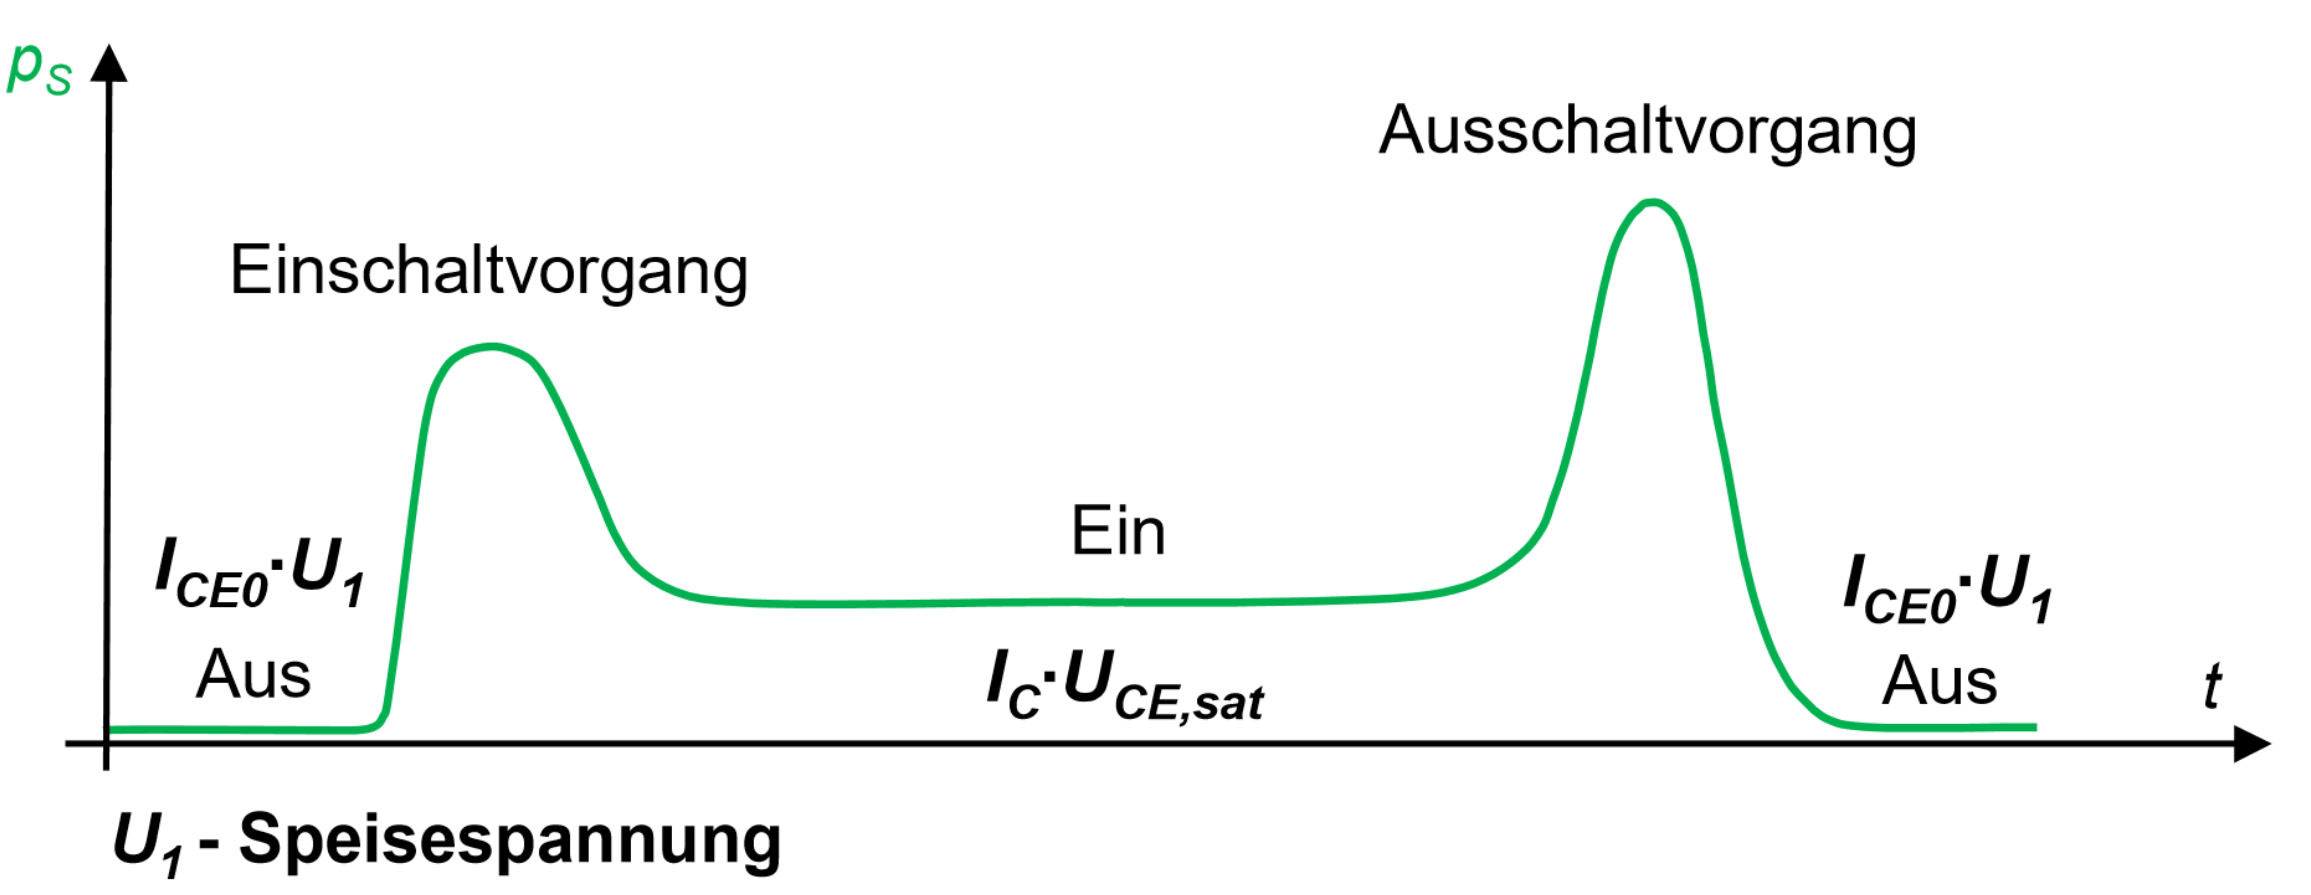
\includegraphics[width=\linewidth]{images/npnTransVerluste}
\end{minipage}
\clearpage

\vspace*{-1cm}
\subsection{Darlington-Transistoren}
%\begin{wrapfigure}{r}{2cm}
%    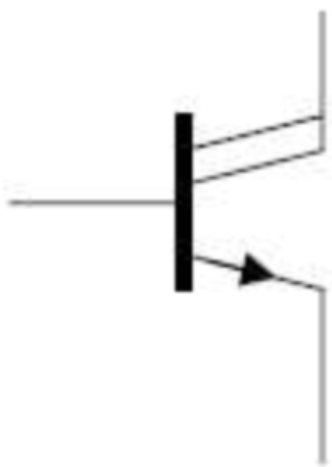
\includegraphics[width=\linewidth]{images/darlingtonSymbol}
%\end{wrapfigure}
Der Stromverstärkungsfaktor der Leistungstransistoren ist relativ klein. Deswegen ist ein starker Basisstrom für diese Transistoren notwendig. Ein Darlington-Transistor löst dieses Problem.\\[0.1cm]
\begin{minipage}{0.6\linewidth}
    \subsubsection{Formeln}
    \vspace{-0.2cm}
    $ \beta = \text{Kleinsignalverstärkung}$\newline
    $B = \text{Grosssignalverstärkung}$
    \vspace{-0.2cm}
    \[ \beta_1 = \dfrac{i_{C1}}{i_{B1}}, \qquad \beta_2 = \dfrac{i_{C2}}{i_{B2}} \]    
    \[ i_{E1} = i_{C1}+i_{B1}=(1+\beta_1)i_{B1} = i_{B2} \]
    \[ i_{C2} = \beta_2 i_{B2} = \beta_2 i_{E1} = \beta_2 (1 + \beta_1)i_{B1}=\beta_{ges}i_{B1} \]
    \[ \beta_{ges} = \beta_2(1 + \beta_1) \approx \beta_1 \beta_2 \]    
\end{minipage}
\begin{minipage}{0.3\linewidth}
    \subsubsection{Aufbau}
    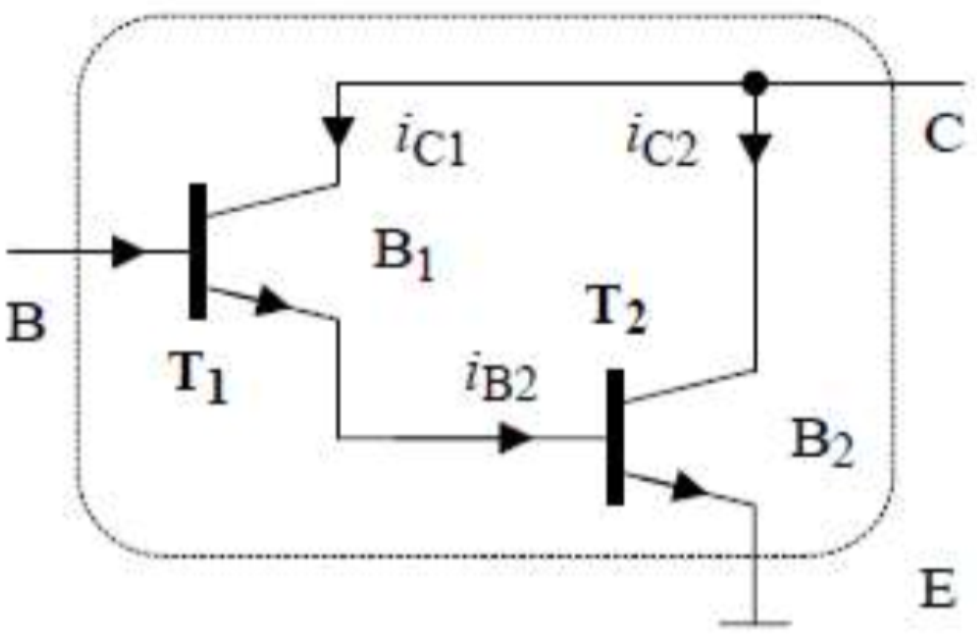
\includegraphics[width=4cm]{images/darlingtonaufbau}
     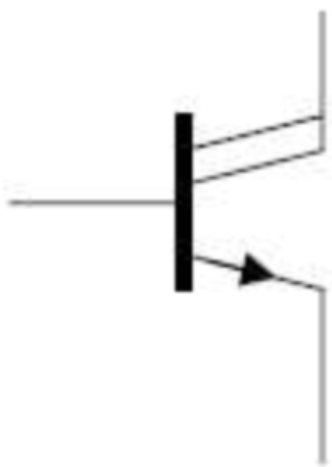
\includegraphics[width=1.5cm]{images/darlingtonSymbol}
\end{minipage}
 \vspace{-0.2cm}
\subsubsection{Vor und Nachteile}
\vspace{-0.5cm}
\begin{multicols}{2}
    \begin{minipage}{\linewidth}
        \begin{itemize}
            \item [+] Gleichbleibender Platzbedarf
            \item [+] höhere Stromverstärkung
            \item [+] $ B \approx B_1 \cdot B_2 $ im Bereich <1000 
            \item [+] $ \beta \approx \beta_1 \cdot \beta_2 $ im Bereich <50'000
        \end{itemize}
    \end{minipage}
    
    \begin{minipage}{1.2\linewidth}
        \begin{itemize}
            \item [-] grosse Phasenverschiebung
            \item [-] für Hochfrequenzanwendungen ungeeignet
            \item [-] langsame Schaltzeiten
            \item [-] doppelte Basis-Emitter-Spannung
        \end{itemize}
    \end{minipage}
\end{multicols}
Für effiziente Schaltanwendungen eignen sich Darlingtontransistoren wegen diesen Nachteilen kaum.
 \vspace{-0.2cm}
\subsection{MOSFET}
\begin{wrapfigure}{r}{7cm}
    \vspace{-1cm}
    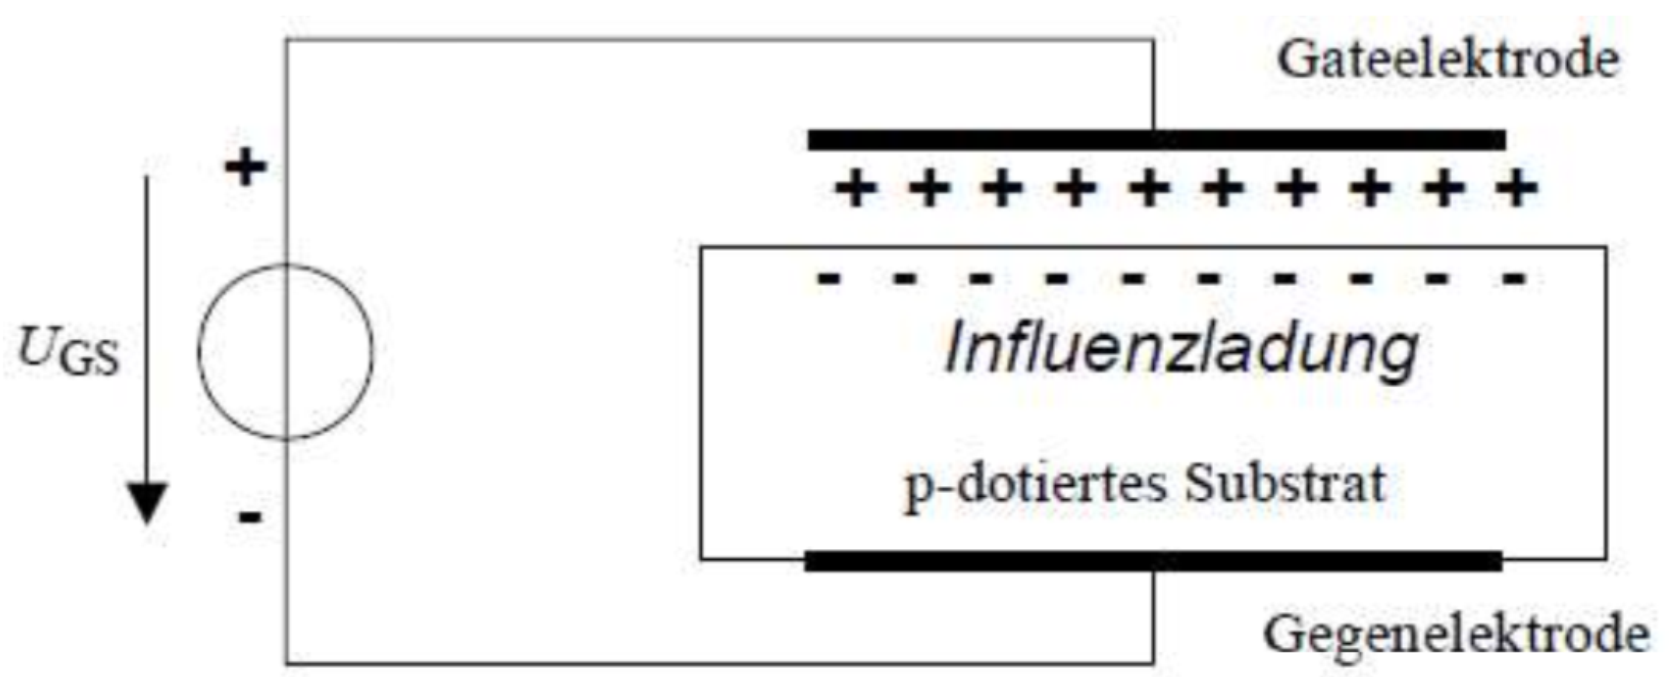
\includegraphics[width=\linewidth]{images/mosfetprinz}
    \newline
    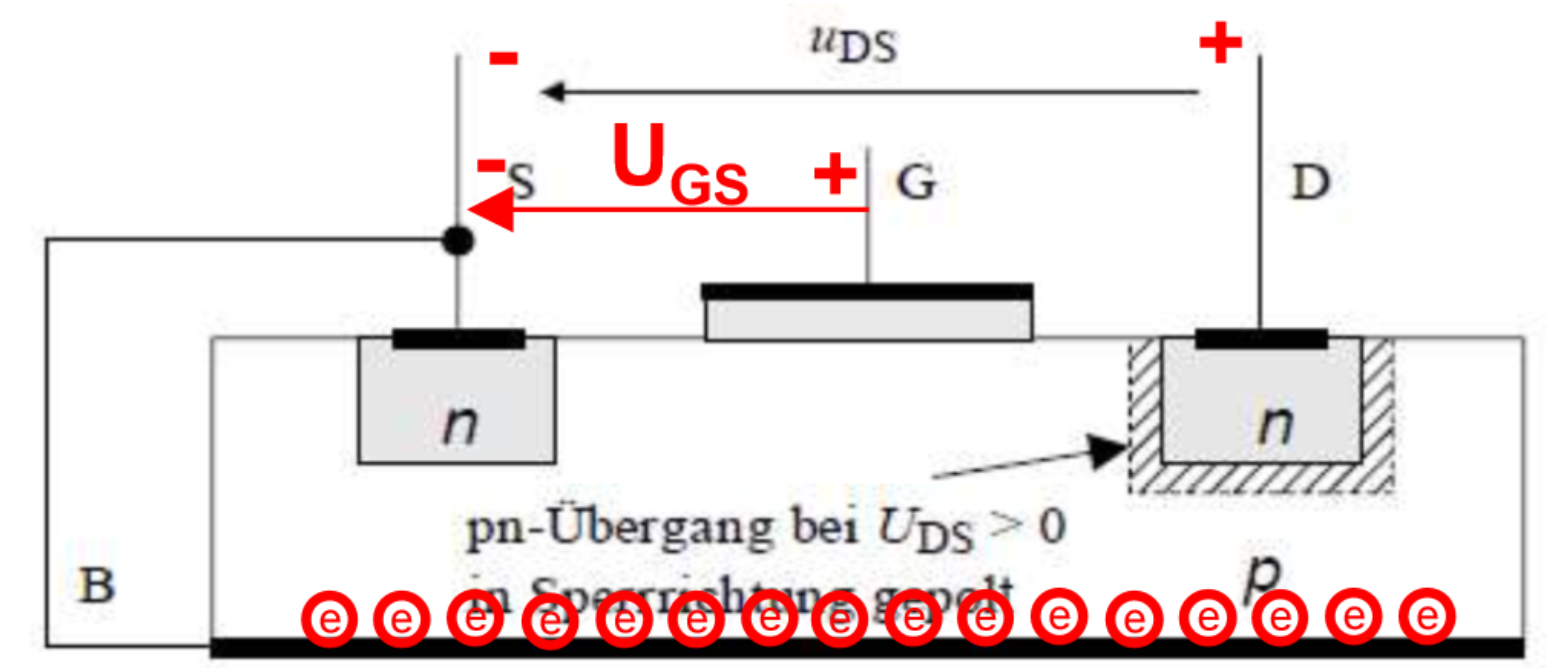
\includegraphics[width=\linewidth]{images/mosfetprak}
\end{wrapfigure}
Die elektrische Leitfähigkeit des Substrats ist durch ein el. Feld \mbox{gesteuert}. Das el. Feld ruft im Substrat eine Influenzladung hervor.\newline
Die Gate-Elektrode ist durch ein Metalloxid vom Substrat isoliert.\\[0.3cm]
\begin{tabular}{ll}
    S = Source & D = Drain\\
    G = Gate & B = Bulk (Substrat)\\
\end{tabular}\\[0.3cm]
$ U_{DS} $ ist positiv damit ist der rechte pn-Übergang in Sperrrichtung \mbox{gepolt}. Deswegen kann kein Strom in beide Richtungen fliessen.\newline
$ \rightarrow $ Der Transistor ist selbstsperrend.\newline
\danger~Sobald eine positive Spannung zwischen $ G $ und $ S $ angelegt ist, entsteht ein leitfähiger n-Kanal und damit auch ein Strom vom \\D- zum S-Anschluss.
 \vspace{-0.2cm}
\subsection{IGBT}
\mbox{Der IGBT setzt such aus einem Bipolartransistor $ T_2 $ und einem MOSFET $ T_1 $ zusammen.}\newline
   \mbox{ \textbf{n- }ist eine schwach dotierte Zone, welche zur Erhöhung der Spannungsfestigkeit verwendet wird.}
\begin{center}
  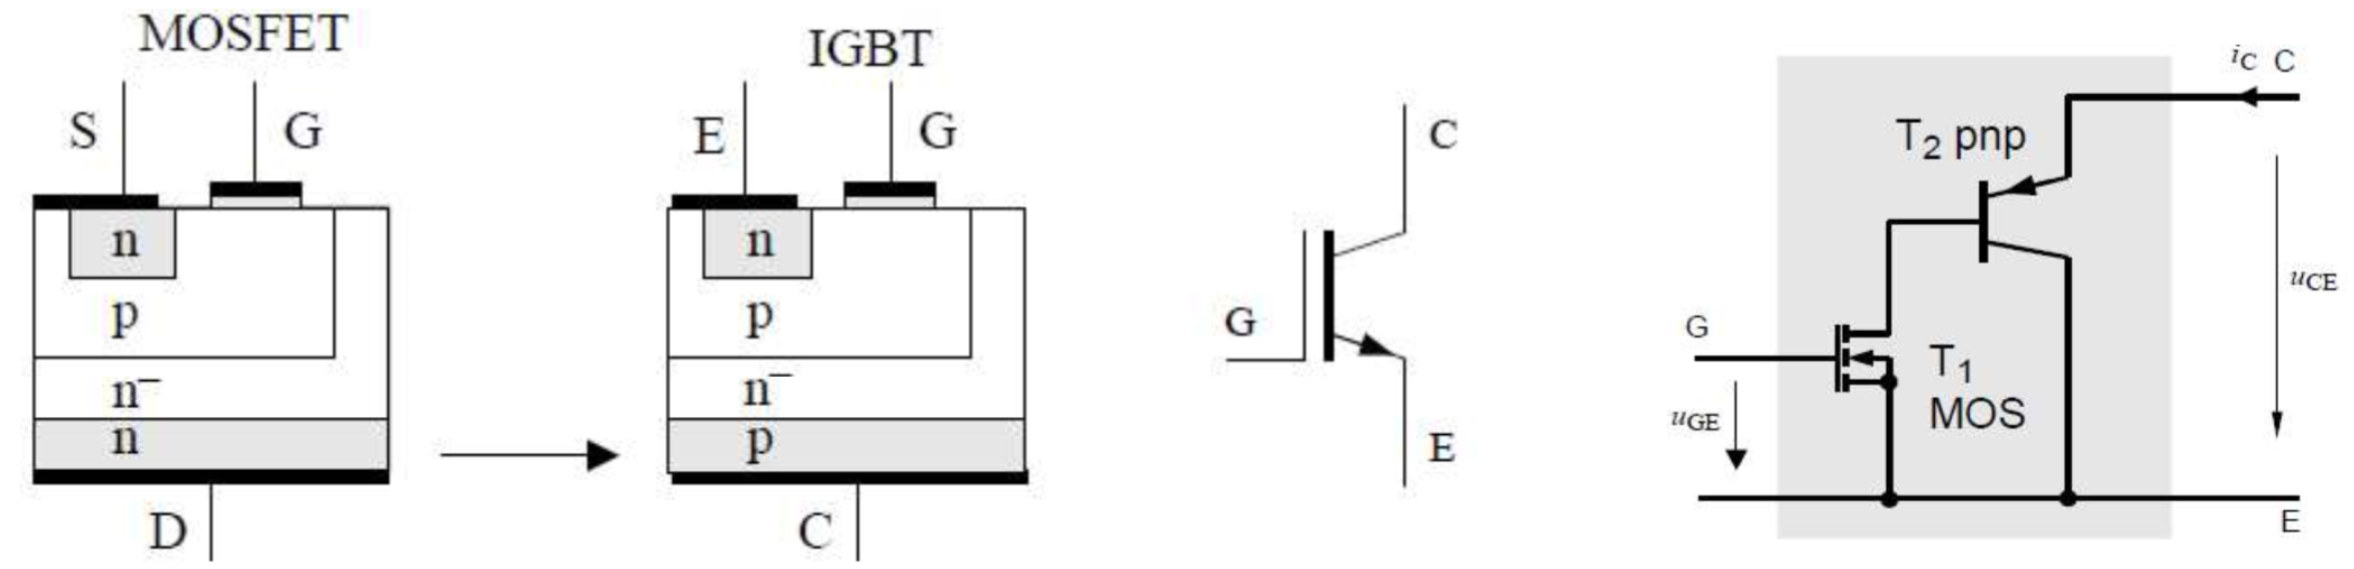
\includegraphics[width=0.7\linewidth]{images/IGBTaufbau}
  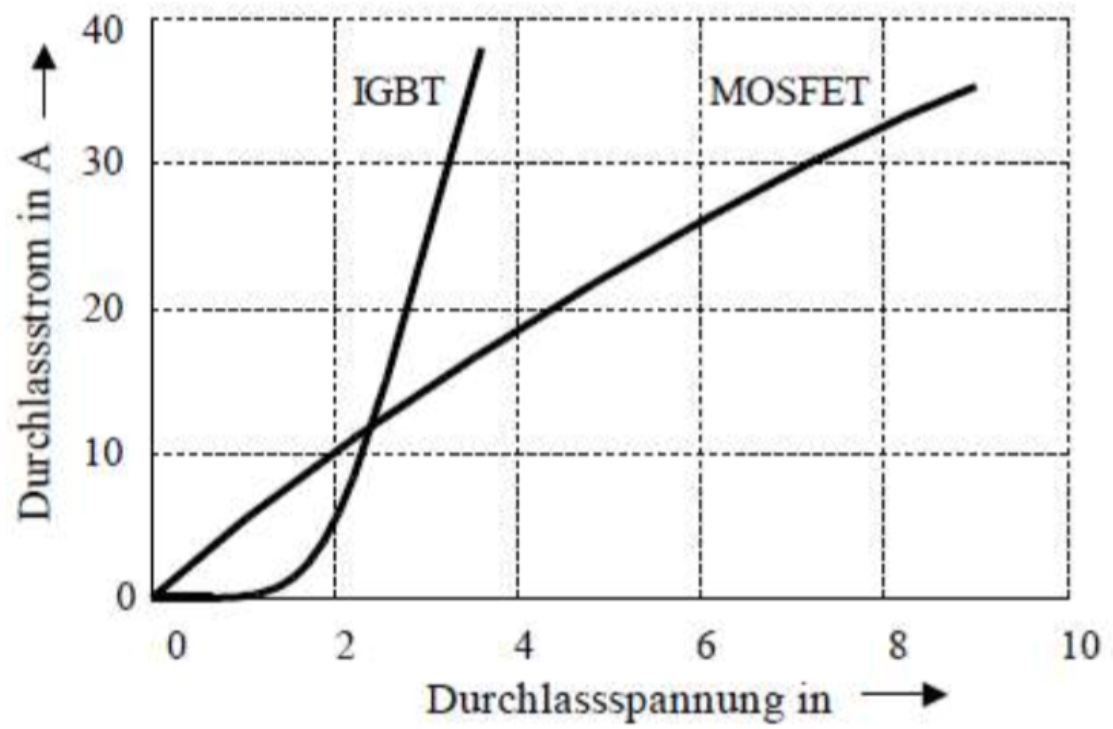
\includegraphics[width=0.25\linewidth]{images/IGBTkennlinie}
\end{center}
\vspace{-0.5cm}
\subsubsection{Eigenschaften}
\begin{multicols}{2}
    \begin{itemize}
        \item \mbox{Über die Kollektor-Emitter-Strecke fällt} \newline \mbox{mindestens die Schleusenspannung ab}
        \item Kleine Durchlassverluste bei hohen Strömen
        \item In Rückwärtsrichtung nur begrenzt sperrfähig
        \item Grosse Sperrverluste vorallem beim Abschalten
    \end{itemize}
\end{multicols}
\clearpage

\subsection{Transistoren im Vergleich}
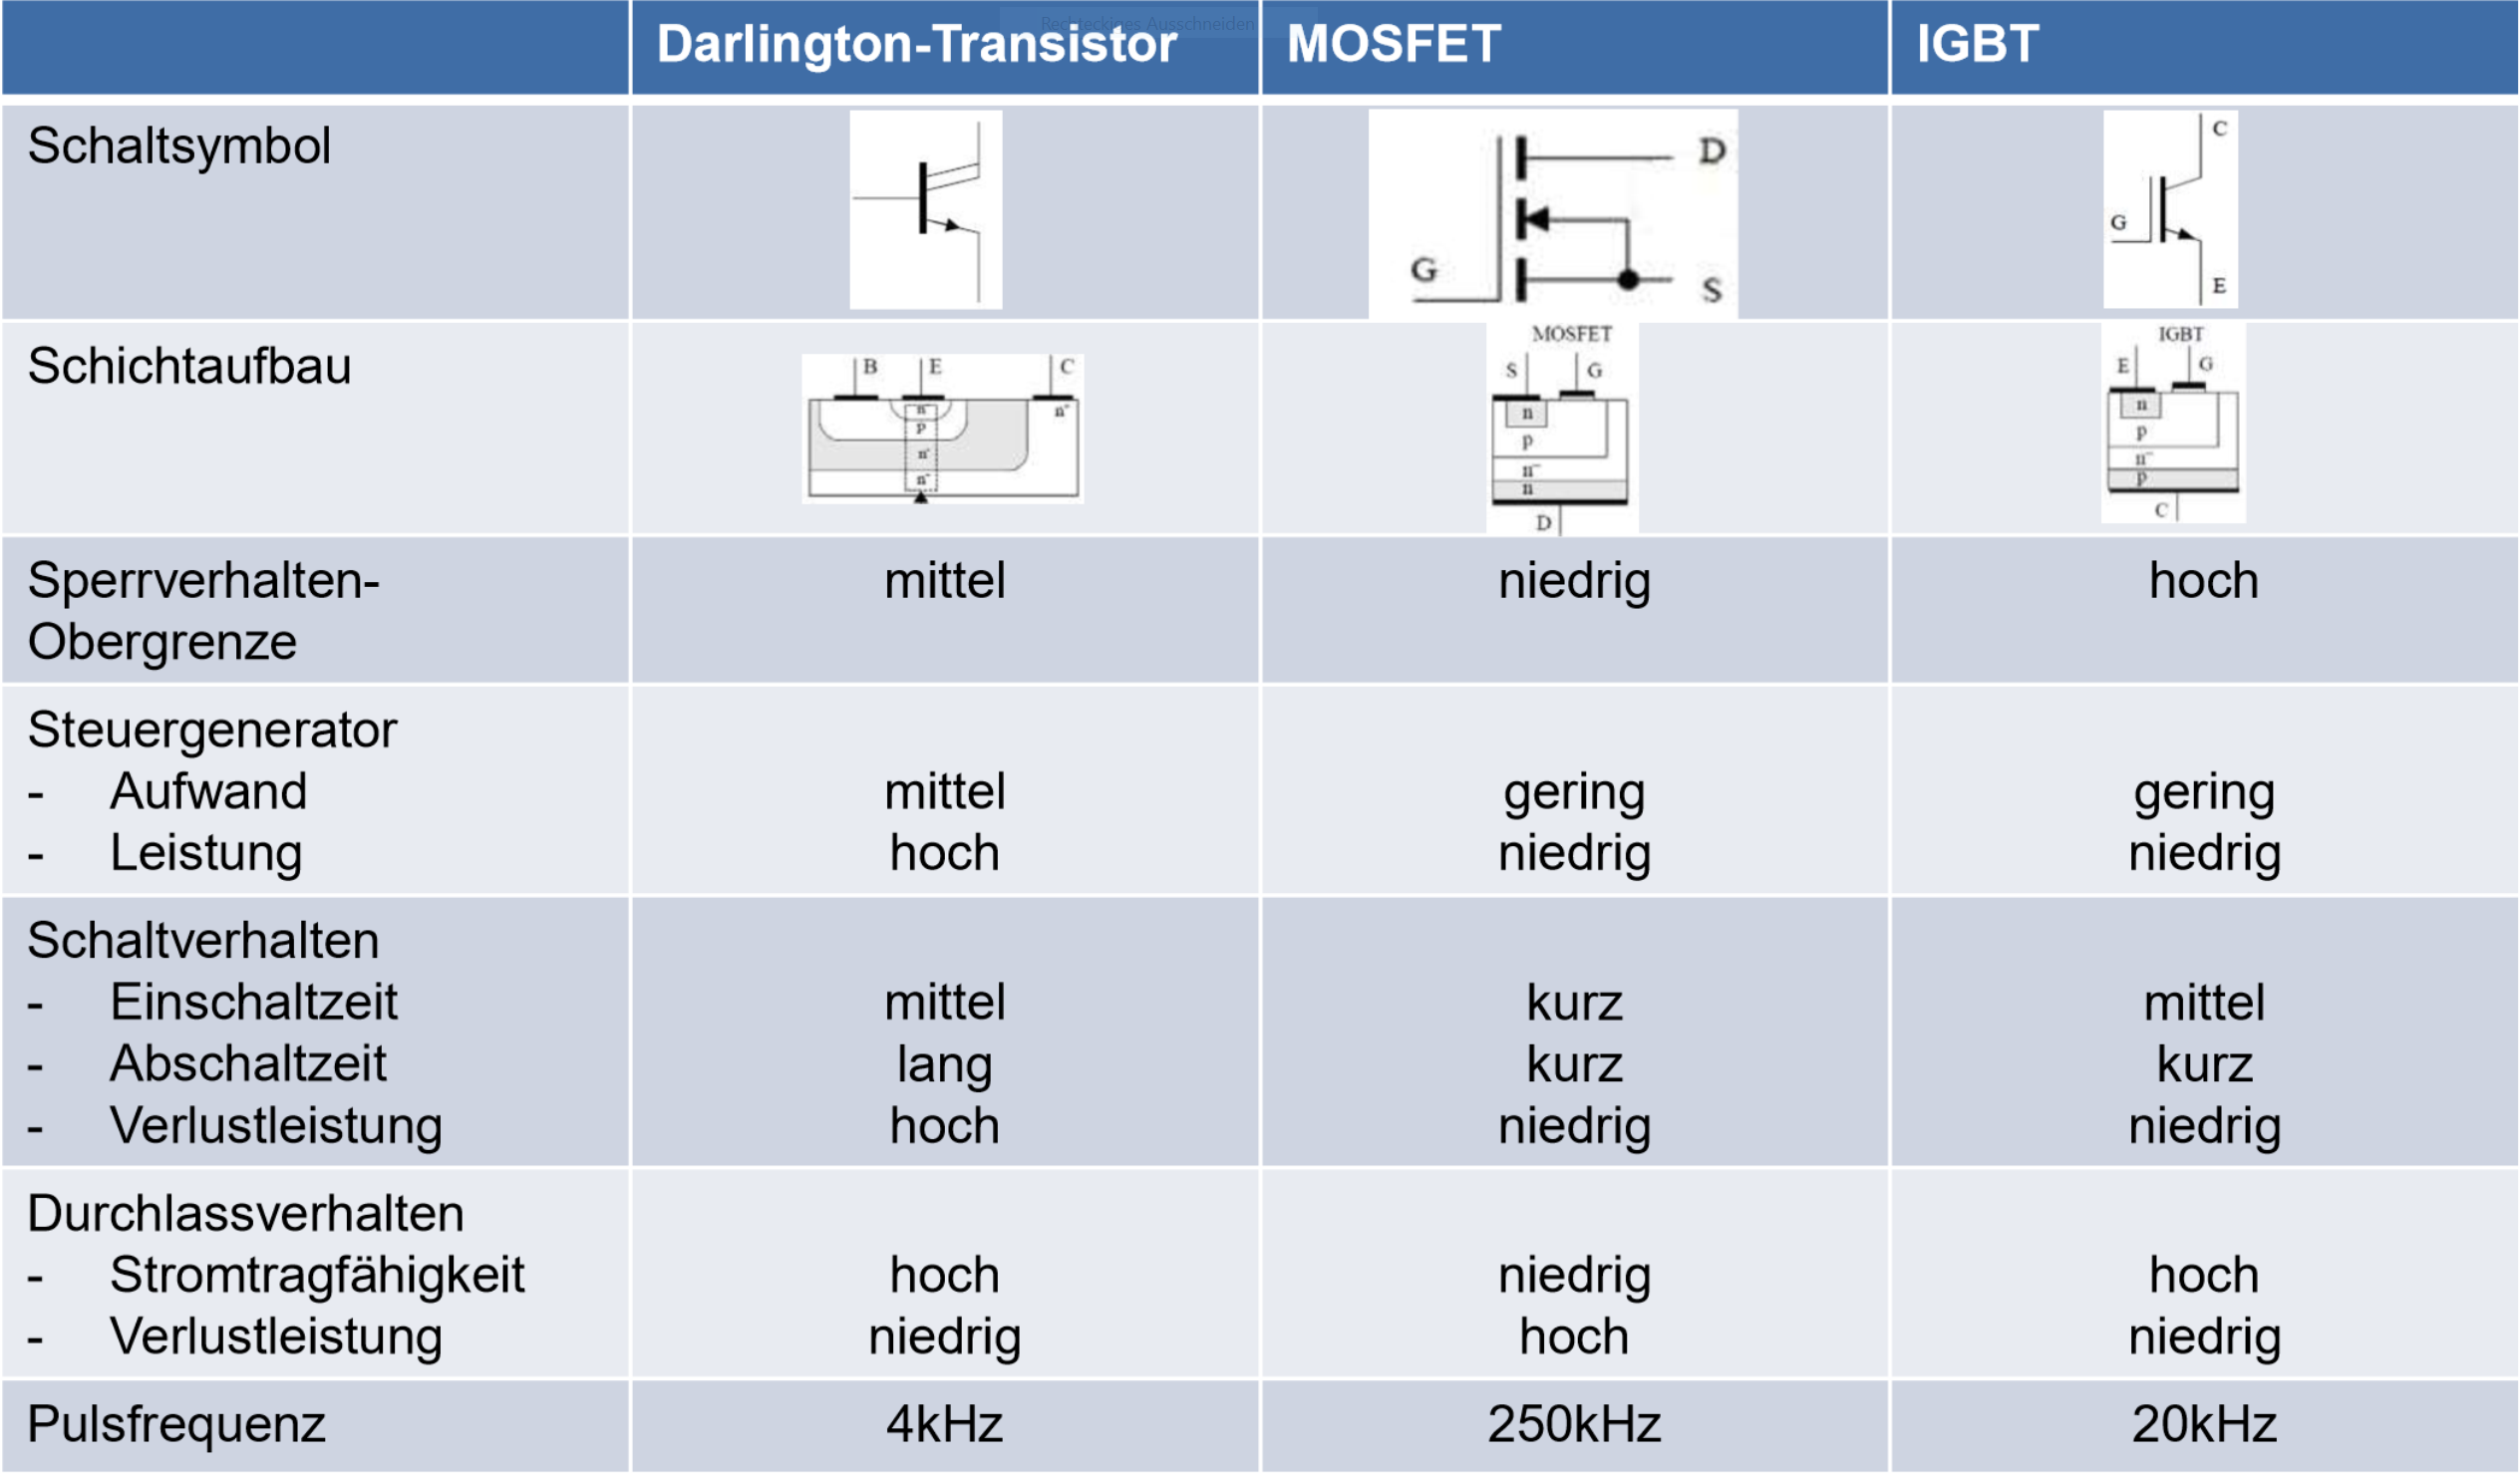
\includegraphics[width=\linewidth]{images/transdiff}
%\begin{tabular}{lccc}
%    &\textbf{Darlington-Transistor}&\textbf{MOSFET}&\textbf{IGBT}\\
%    Schaltsymbol&
%    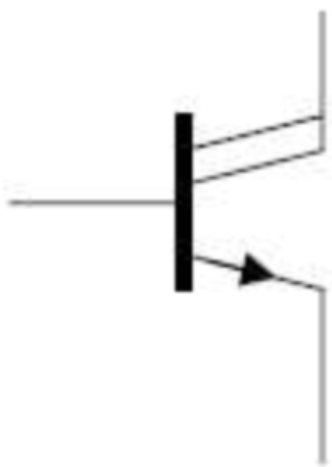
\includegraphics[width=1cm]{images/darlingtonSymbol}&
%    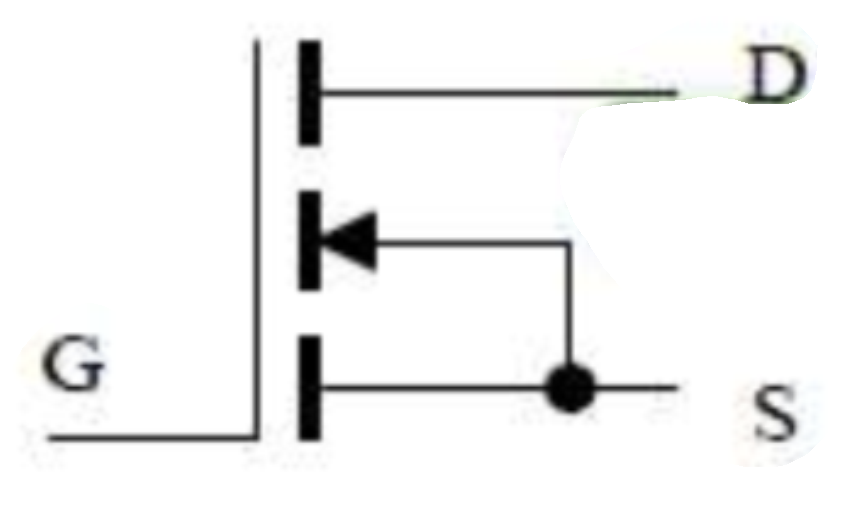
\includegraphics[width=2cm]{images/MOSFETSymbol}&
%    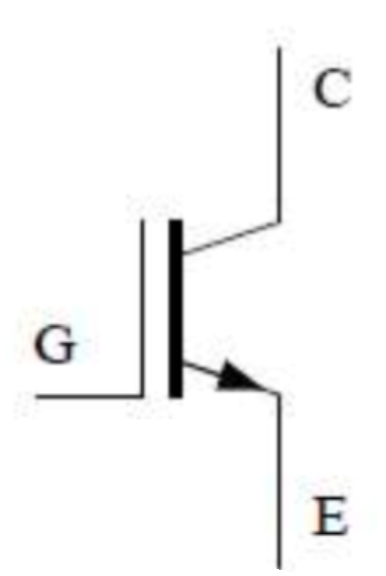
\includegraphics[width=1cm]{images/IGBTSymbol}\\
%    
%    Schichtaufbau&
%    \includegraphics[width=1cm]{images/darlingtonSchicht}&
%    \includegraphics[width=1cm]{images/MOSFETSchicht}&
%    \includegraphics[width=1cm]{images/IGBTSchicht}\\
%    
%    &&&\\
%    &&&\\
%    &&&\\
%    &&&\\
%    &&&\\
%    &&&\\    
%\end{tabular}

%=========================================
\clearpage
\begin{minipage}{0.7\linewidth}
\section{Thyristoren}
Ein Thyristor besteht aus vier Halbleiterschichten d.h. aus drei pn-Übergängen \newline
Thyristoren sind einschaltbare Bauelemente.\newline
Thyristoren sind  \"{}einschaltbare Dioden\"{}. Thyristoren werden mit dem \newline Zündimpuls der zwischen Gate (G) und Kathode (K) kurzzeitig anliegt durchgeschaltet.
\end{minipage}
\begin{minipage}{0.3\linewidth}
     \hspace{1cm}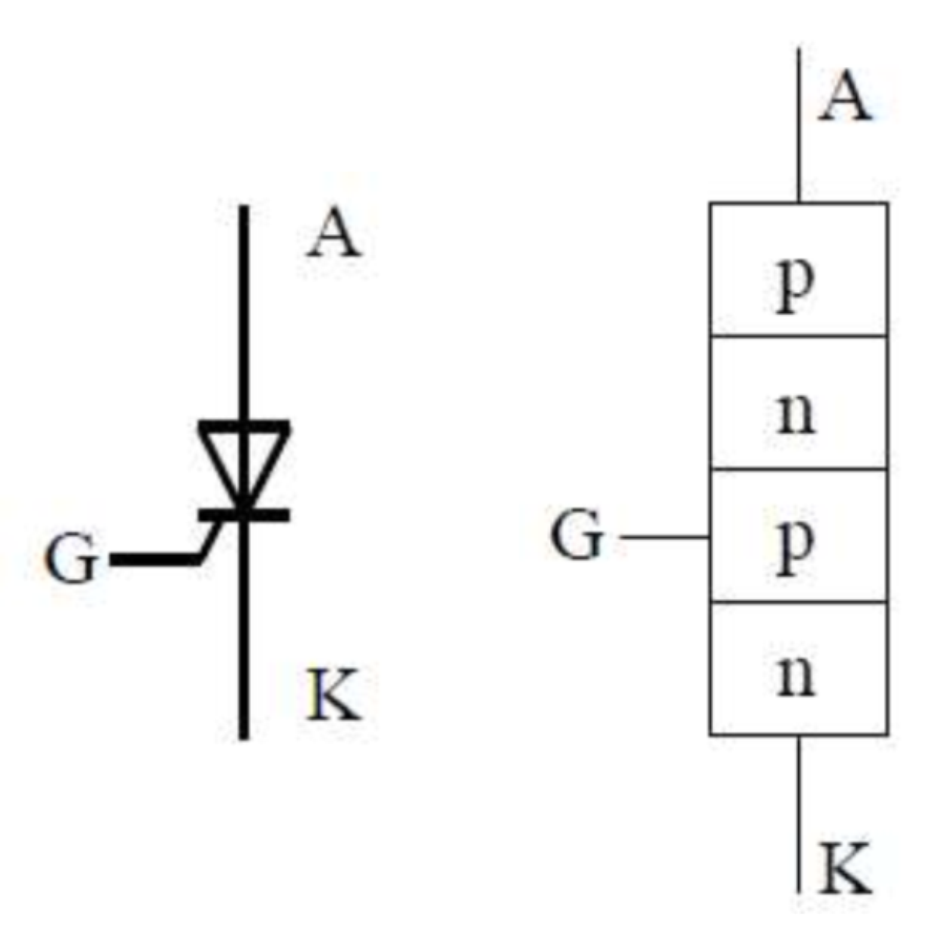
\includegraphics[width=0.5\linewidth]{images/thyraufbau}
\end{minipage}
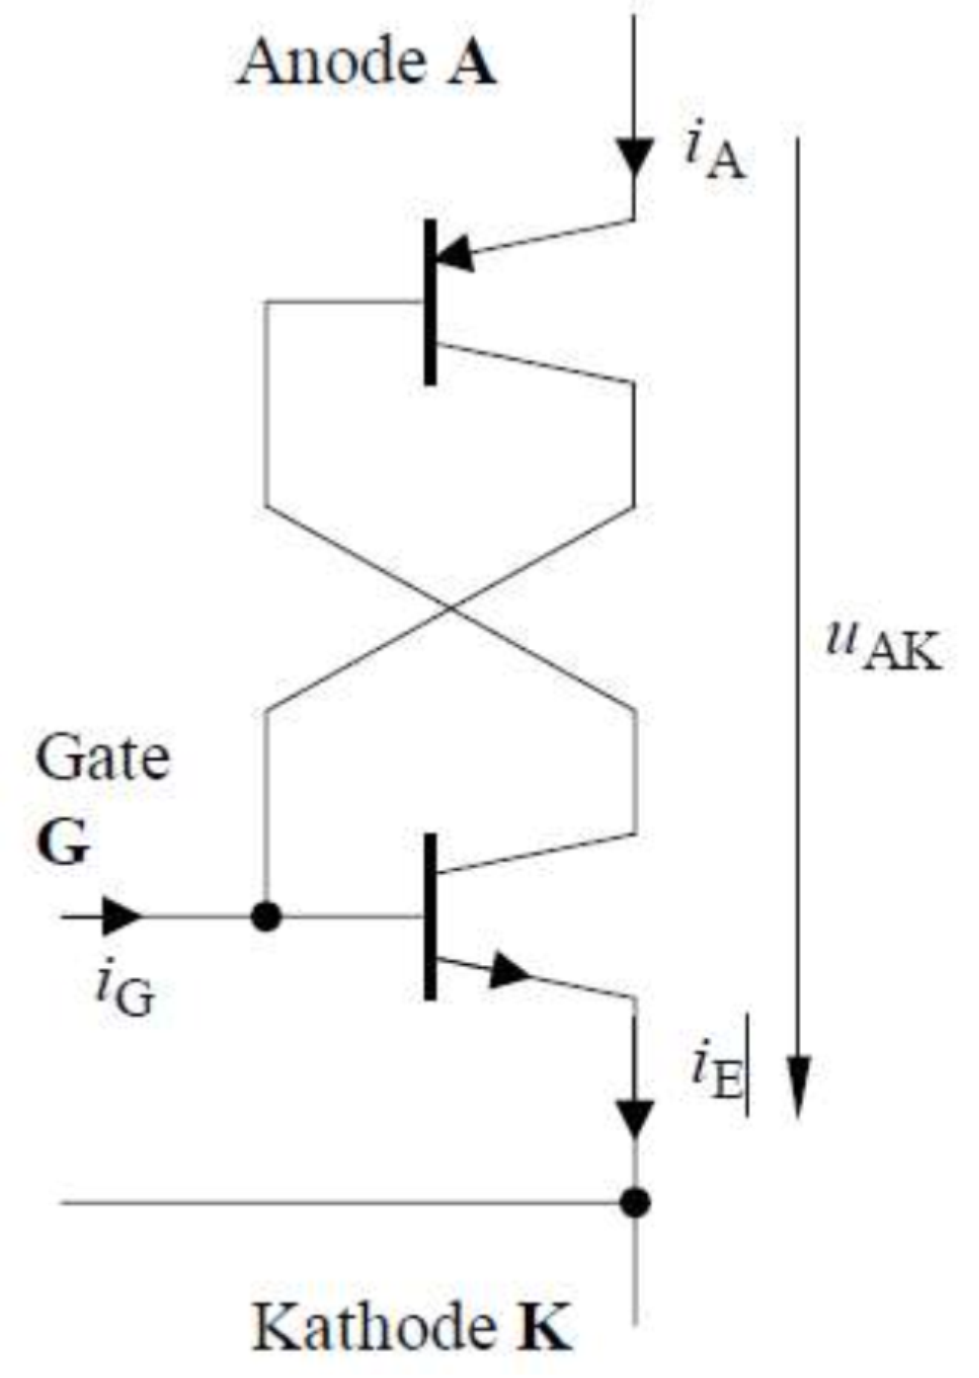
\includegraphics[width=0.15\linewidth]{images/thyrESB}
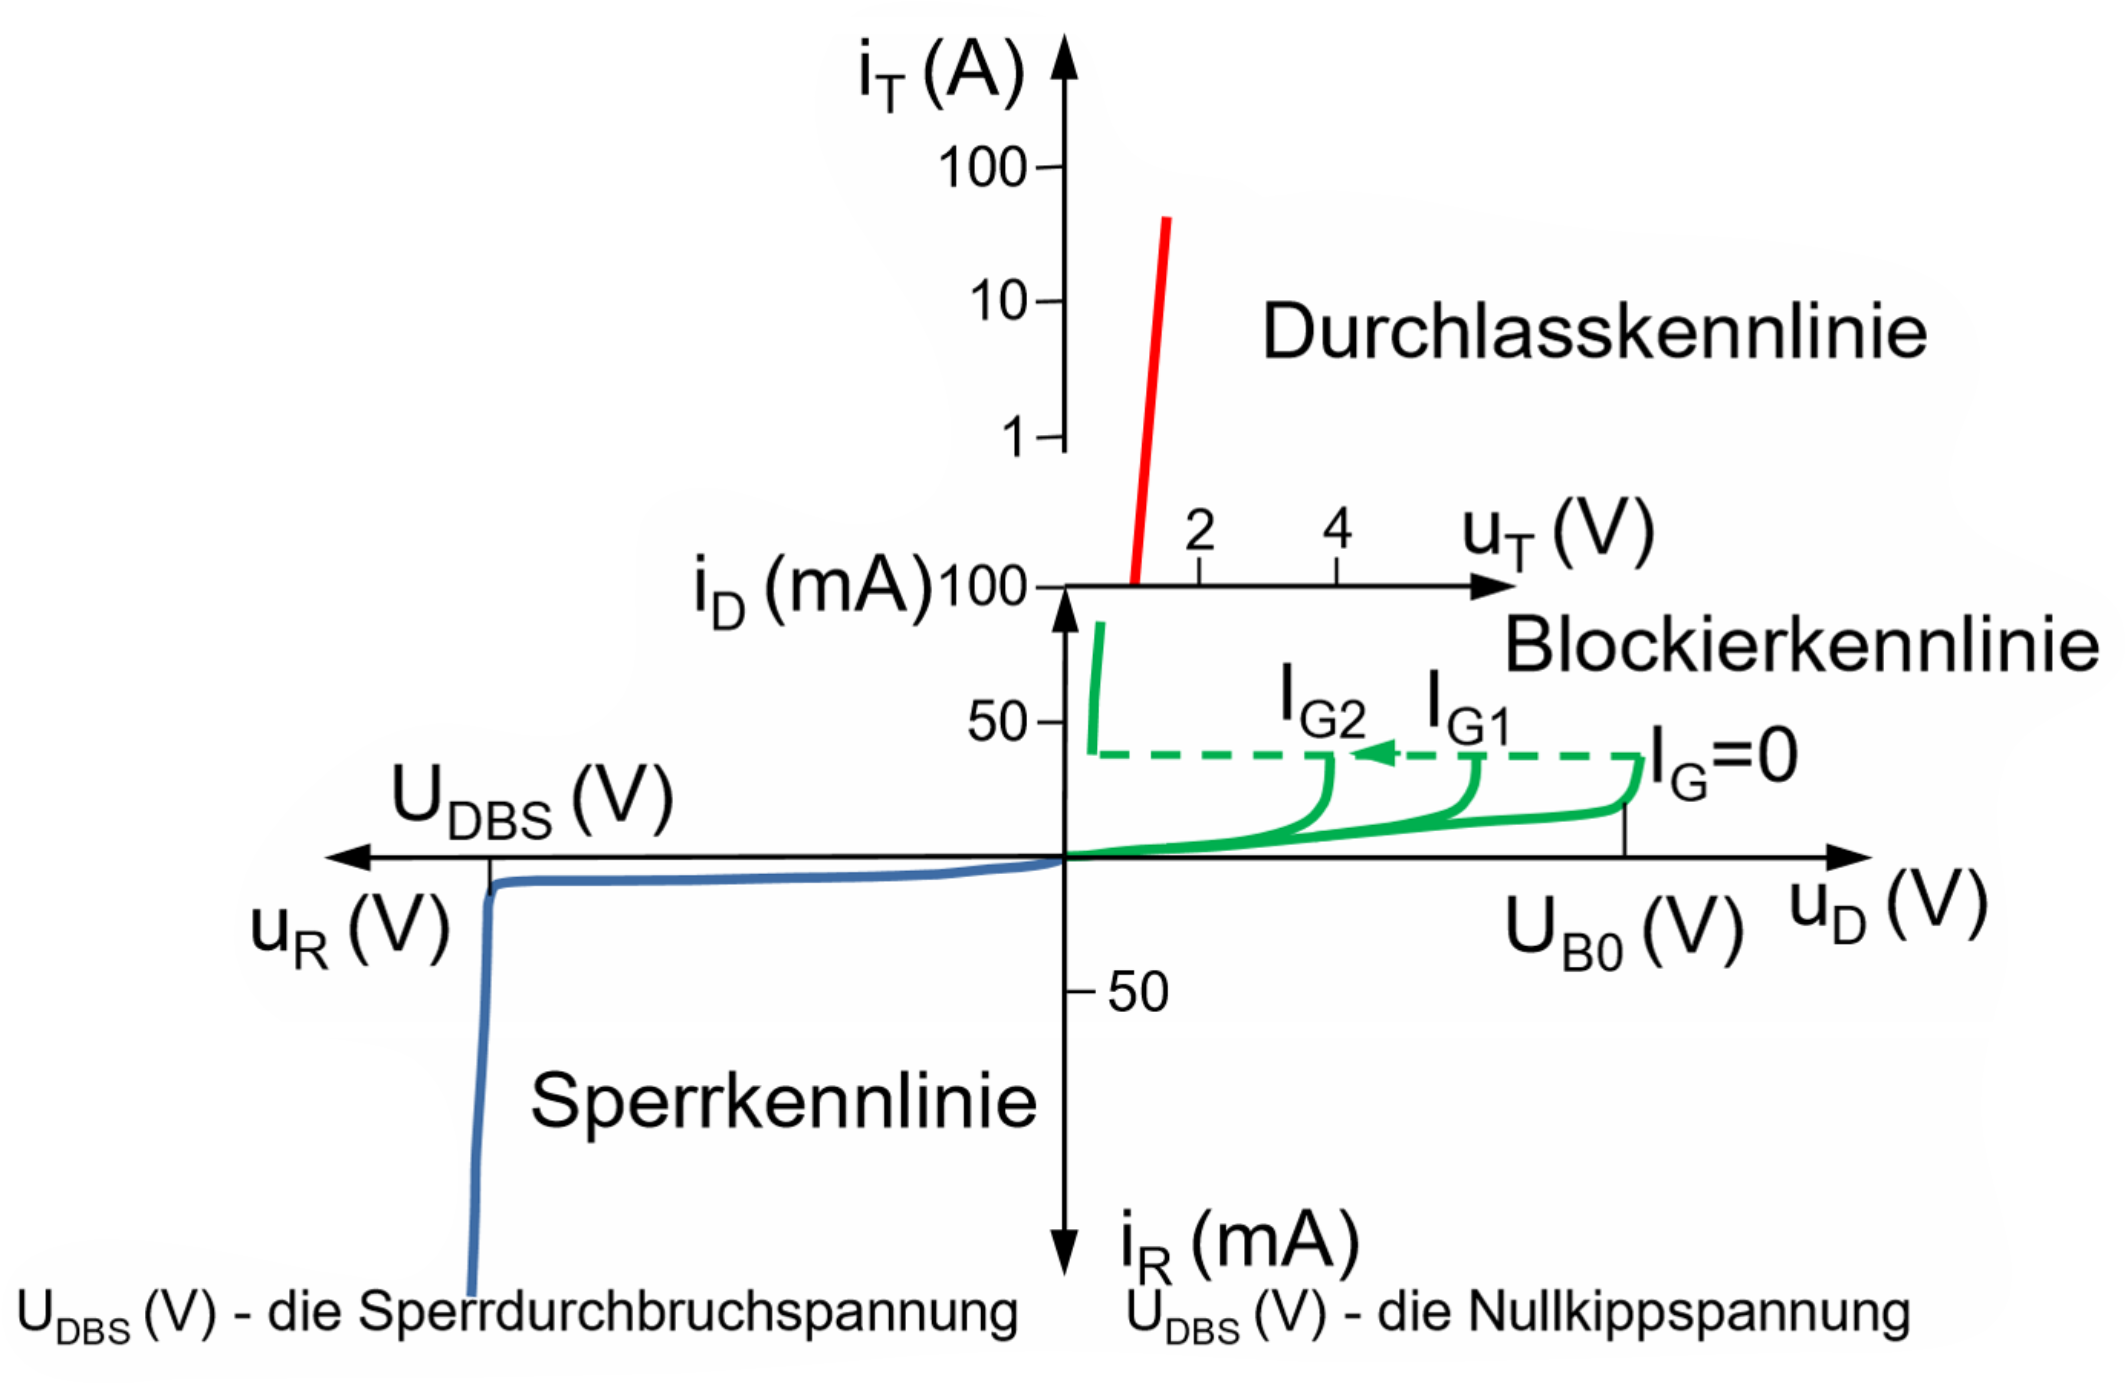
\includegraphics[width=0.4\linewidth]{images/thyrKennlinie}
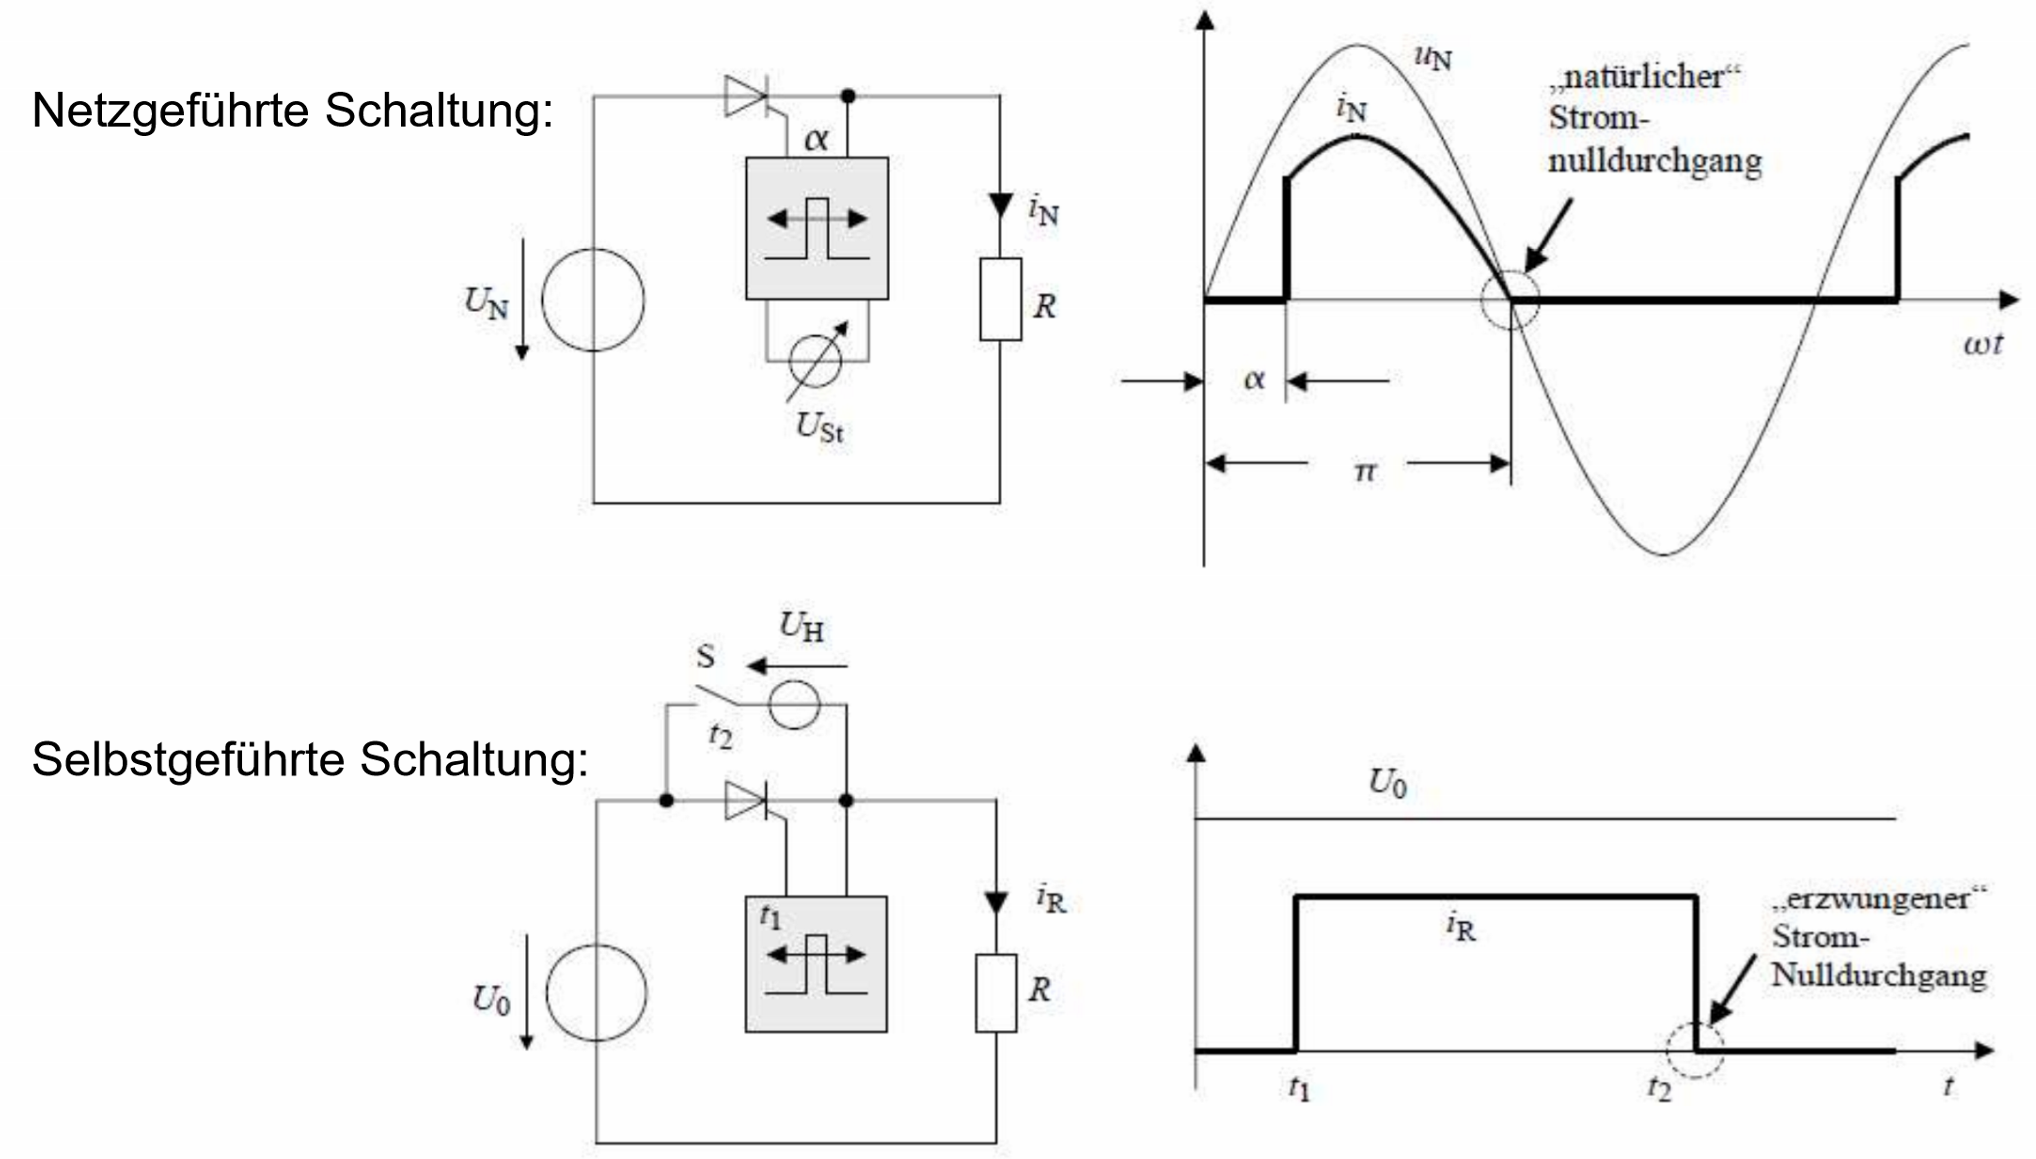
\includegraphics[width=0.45\linewidth]{images/thyrSchaltung}
\subsection{Thermische Ersatzschaltung}

\begin{multicols}{3}
    \begin{minipage}{\linewidth}
        \textbf{Thermische Kenngrösse}\newline
        Wärmeleistung P [W]\newline
        Temperaturunterschied $ \vartheta $ [K]\newline
        Wärmewiderstand $ R_{th} $ [${K}/{W}$]\newline
        \textbf{Elektrische Kenngrösse}\newline
        Strom I  [A]\newline
        Spannung [V]\newline
        Widerstand [$\nicefrac{V}{A}, \Omega$]\newline
    \end{minipage}
	\begin{minipage}{\linewidth}
		\subsubsection{Thyristor ohne Kühlung}
		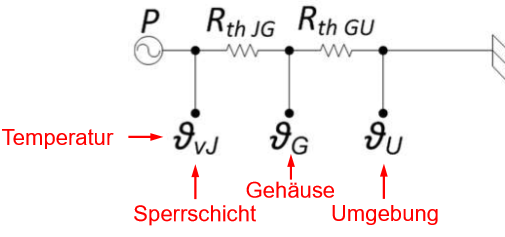
\includegraphics[width=\linewidth]{images/thyrOK}
		\[ \vartheta_{vJ}-\vartheta_U=P \cdot (R_{th\; JG}+R_{th\; GU}) \]		
	\end{minipage}
	\begin{minipage}{\linewidth}
		\vspace{0.2cm}
		\subsubsection{Thyrisor mit Kühlung}
		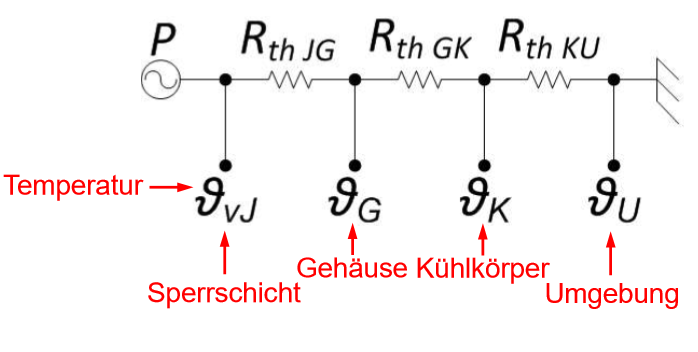
\includegraphics[width=\linewidth]{images/thyrMK}
		\[ \vartheta_{vJ}-\vartheta_U=P \cdot (R_{th\; JG}+R_{th\; GK}+R_{th\; KU}) \]	
        \[ R_{th \; KU}=\dfrac{\Delta \vartheta}{P} \]
	\end{minipage}
\end{multicols}
\vspace{-1.5cm}
\textbf{Beispiel Schaltverluste bei B2C}\newline
\begin{tabular}{ll}
    Spitzenwert des Thyristorstromes&
    $\widehat{I}_{R} = \frac{\widehat{U}_{2}}{R}$\\
    \\
    
    Mittelwert des Thyristorstromes &
    $I_{T AV} = \frac{1}{2\pi}\int\limits_{\alpha}^{\pi}I_{Rm} \cdot sin(\beta) \cdot \diff\beta= \frac{\hat{I}_{R}}{2\pi} \cdot (1+cos\alpha)$\\
    \\

    Effektivwert des Thyristorstromes &
    $I_{T RMS} = \sqrt{\frac{I_{RM}^2}{2\pi}\int\limits_{\alpha}^{\pi}sin^2(\beta)\diff\beta}= \frac{\hat{I}_{R}}{2}\sqrt{\frac{\pi - \alpha}{\pi}+\frac{sin2\alpha}{2\pi}}$\\

    momentane Verlustleistung:&
    $p(t) = u_{T}(t) \cdot i_{T}(t)$\\
    Mittelwert der Verlustleistung: &
    $P_{T} = \frac{1}{T}\int\limits_{0}^{T}u_{T}(t) \cdot i_{T}(t) \cdot \diff t = U_{T0} \cdot \frac{1}{T}\int\limits_{0}^{T}i_{T}(t)\diff t+r_{T} \cdot \frac{1}{T}\int\limits_{0}^{T}i_{T}^2(t)\diff t$\\
    \\
    & $P_{T} = U_{T0} \cdot I_{T AV} + r_{T} \cdot I_{T RMS}^2$\\[0.3cm]
\end{tabular}

 $I_{T AV}$ ist der Mittelwert und $I_{T RMS}$ der Effektivwert des Thyristorstroms\\[0.2cm]
\textbf{Der Wert für $U_{T0}$ kann aus dem Datenblatt des Thyristors herausgelesen werden.}\\[0.2cm]

\begin{minipage}{0.5\linewidth}
    \subsection{Abschaltbarer Thyristor}
    \begin{minipage}{0.7\linewidth}        
        \textbf{(GTO = Gate-Turn-Off)}\newline
        Der GTO schaltet aus, wenn ein ausreichend hoher negativer Gate-Strom \newline auftritt.\newline
        Amplitude des Gate-Stromes muss 20\% bis 30\% des abzuschaltenden GTO-Stromes betragen.
    \end{minipage}
    \begin{minipage}{0.2\linewidth}
        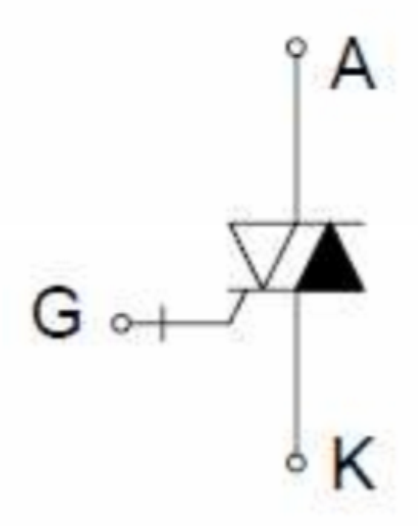
\includegraphics[width=\linewidth]{images/GTOSymbol}
    \end{minipage}    
\end{minipage}
\begin{minipage}{0.5\linewidth}
    \subsection{IGCT}
    	        \begin{wrapfigure}{r}{1.5cm}
    	        	\vspace{-1cm}
    	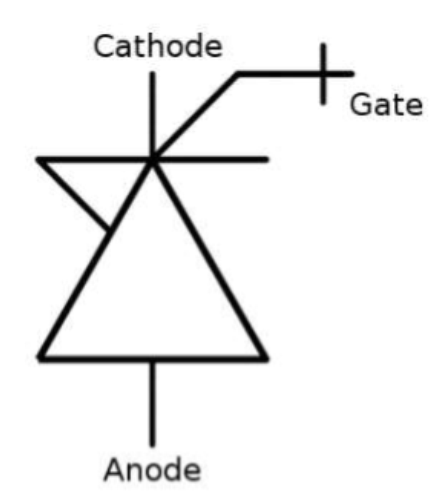
\includegraphics[width=\linewidth]{images/IGCTSymbol}
    \end{wrapfigure} 
    \begin{minipage}{\linewidth}
        \textbf{Integrated Gate-Commutated Thyristor}\\
        IGCT sind die Weiterentwicklung der GTO.\newline
        Sie werden hauptsächlich für Mittel\-spannungs\-umrichter eingesetzt.
    \end{minipage}
\end{minipage}
\clearpage

\section{Stromrichterschaltung}
\subsection{Gruppierung}
\subsubsection{nach Steuerung}
\begin{itemize}
    \item Ungesteuerte Stromrichter:
        \subitem Das Verhältnis von Eingangs- zu Ausgangsspannung wird durch die Stromrichterschaltung festgesetzt
    \item Gesteuerte Stromrichter
        \subitem Das Verhältnis von Eingangs- zu Ausgangsspannung wird durch Steuereingriff am Halbleiterschalter verändert. 
\end{itemize}

\subsubsection{nach Führung}
\href{https://de.wikipedia.org/wiki/Kommutierung}{Kommutierung WIKI}\newline
\begin{minipage}{0.6\linewidth}
Bzw. nach der Herkunft der Kommutierungsspannung.\newline
Kommutierung bedeutet die Wechslung des Stromflusses von einem HL-Ventil auf ein Anderes.
\begin{itemize}
    \item Netzgeführte Schaltung
        \subitem Kommutierungsspannung vom Netzwerk
    \item Lastgeführte Schaltung
        \subitem Kommutierungsspannung wird durch Lastkreis\\
        (z.B. Synchronmotor) gesteuert
    \item Selbstgeführte Schaltung
        \subitem Kommutierungsspannung wird selbst erzeugt
\end{itemize}
\end{minipage}
\begin{minipage}{0.4\linewidth}
    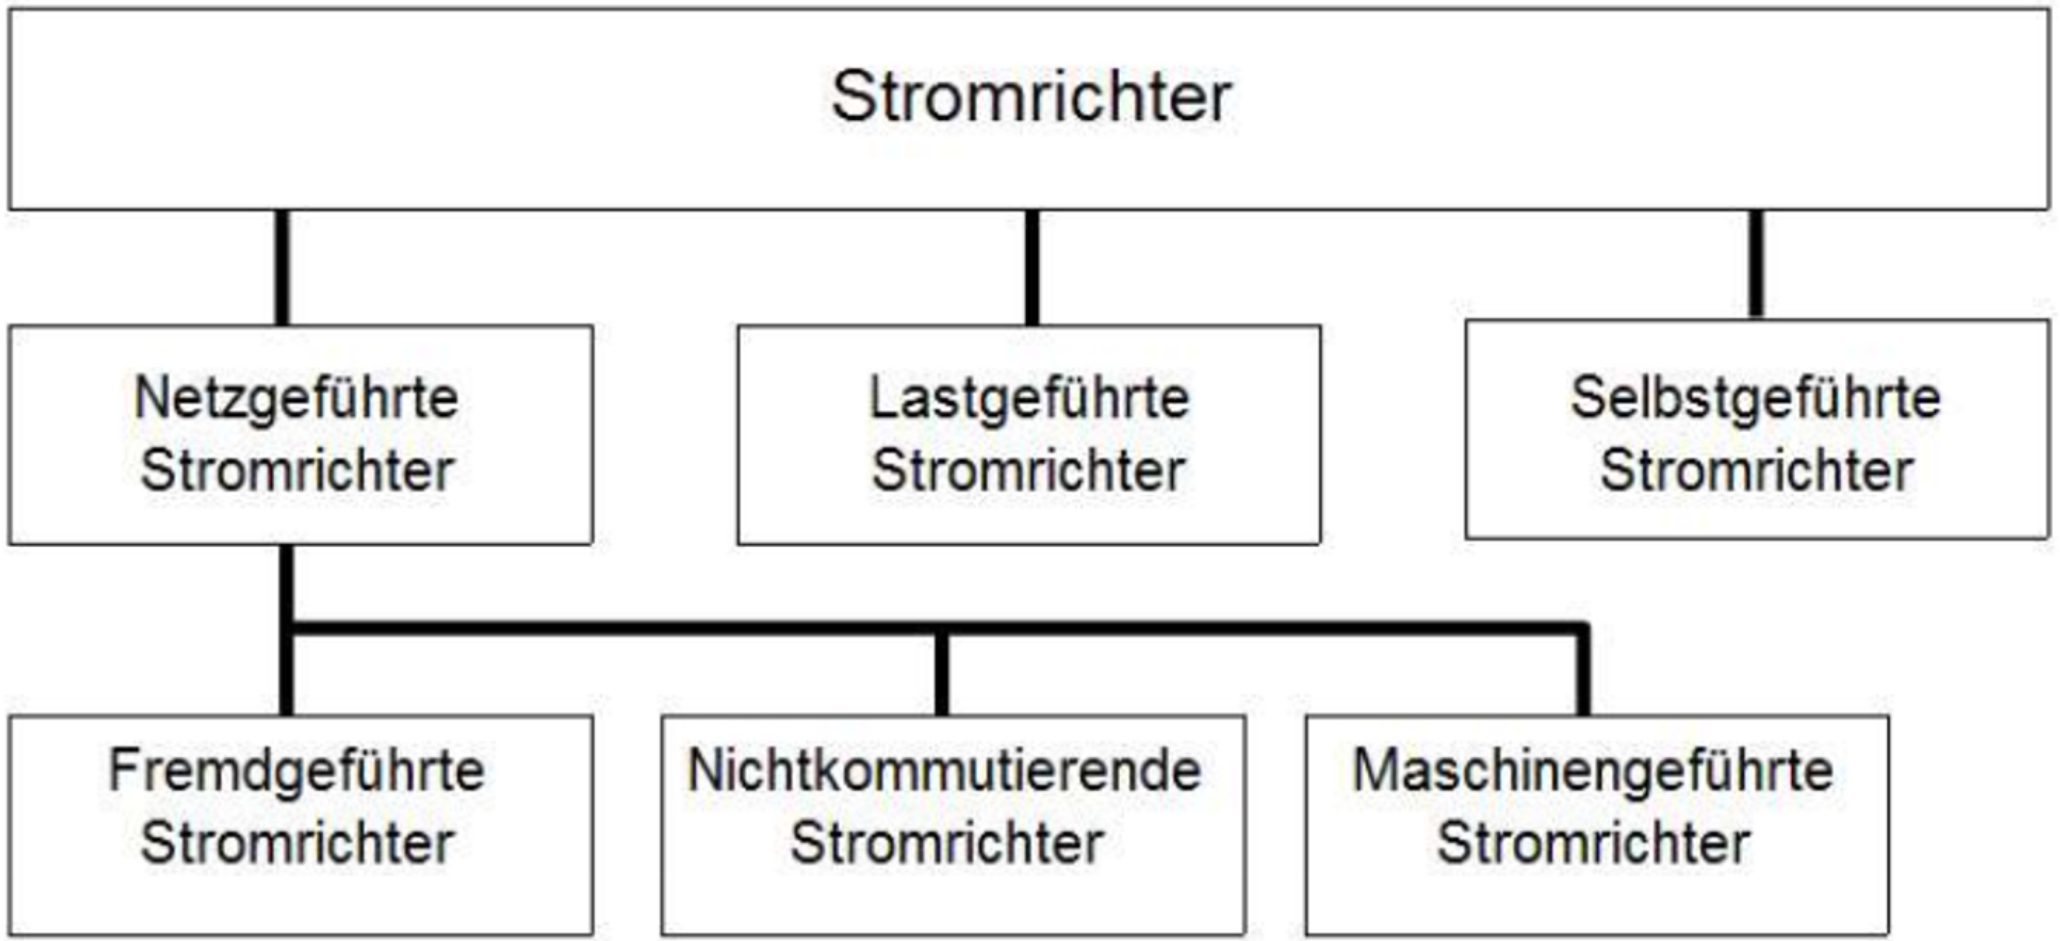
\includegraphics[width=\linewidth]{images/StromrichterKennzeichnung}\newline
\end{minipage}

\subsection{Kennzeichnung}
\includegraphics[width=0.9\linewidth]{images/SRKennzeichnung}\newline
\href{https://de.wikipedia.org/wiki/Gleichrichter}{Gleichrichter WIKI}

%===================================================================
\clearpage
    \subsection{Ungesteuerter Gleichrichter}
\subsubsection{M1U}
\vspace{-0.5cm}
\begin{minipage}{0.4\linewidth}
    \includegraphics[width=\linewidth]{images/PrakUGM1}
\end{minipage}
\begin{minipage}{0.3\linewidth}
    \centering
   \includegraphics[width=0.7\linewidth]{images/PrakUGM1Kl1}
   \includegraphics[width=0.7\linewidth]{images/PrakUGM1Kl2}
\end{minipage}
\begin{minipage}{0.3\linewidth}
    \includegraphics[width=\linewidth]{images/UGM1OW} 
\end{minipage}
\newline

%\includegraphics[width=0.4\linewidth]{images/UGRM1U}
%\includegraphics[width=0.2\linewidth]{images/UGRM1US} \newline
Die Diode wird als Ideal betrachtet $ \rightarrow $ keine Schwellenspannung oder Innenwiderstand
\begin{longtable}{| p{.33\textwidth} | p{.40\textwidth} | p{.25\textwidth} |} %TODO Formeln einfügen bzw anpassen
    \hline
    \textbf{Grundgleichungen}&
    \[ U_2 = U_D + U_R \]
    \[ U_R = I_2 \cdot R\]
    \[ \bar{U}_{OUT} = \dfrac{\hat{U}}{\pi}\]&\\
    \hline
    \textbf{Durchlassrichtung}\newline
    $ 0 < \omega t < \pi $&
    \vspace{-0.3cm}\[ U_2 = U_R \qquad U_D = 0 \] \vspace{-0.3cm}&\\
    \hline   
    \textbf{Sperrichtung}\newline
    $ \pi < \omega t < 2\pi $&
     \vspace{-0.3cm}\[ U_2=U_D \qquad U_R = 0 \] \vspace{-0.3cm}&\\
    \hline
    
    \textbf{Wirkleistung der Last R}&
    \[ P=\frac{1}{2\pi} \int_{0}^{2\pi} p(\alpha) d\alpha = \dfrac{U_{R\;RMS}^2}{R} \]&
    \\ \hline
%    
%    \textbf{Scheinleistung}&
%    \[ S_2 = U_2 \cdot I_2 = U_2 \cdot I_{R RMS} \]&
%    \\ \hline
%        
%    \textbf{Grundschwingugngsblindleistung}&
%    \[ Q_2 = I_{2 1} \cdot sin(\varphi_{2 1}) = 0 \]&
%    \\ \hline    
%    
%        
%    \textbf{Verzerrungsleistung}&
%    \[ Q_v = U_2 \cdot \sqrt{\sum_{k=2}^{\infty} {I_2^2}_k} = \sqrt{S_2^2 - P_2^2} \]&
%    \\ \hline %STIMMT DIES FORMEL? Siehe Grundformel

\end{longtable}

%
%Leistung = Momentanleistung des Sormes x momentanleistung der Spannung\\
%Leistung = Leistung bei trafoseite messen 1harm des stroms phasenverschiebung -> u i cos(phi) fourierreihen..
%Leistung = Irav* U1harm  
\textbf{Oberwellen}\newline
\vspace{-1cm}
\begin{multicols}{3}
    \textbf{ \qquad R}\newline   
    \includegraphics[width=\linewidth]{images/M1UR}   
    \textbf{\null \qquad R + L}\newline
    \includegraphics[width=\linewidth]{images/M1URL}
    \textbf{ \qquad R + L+ freilaufDiode}\newline
    \includegraphics[width=\linewidth]{images/M1URLD}
\end{multicols}
%===================================================================
\clearpage

\subsubsection{B2U}
\begin{minipage}{0.4\textwidth}
    \includegraphics[width=\linewidth]{images/PrakUGB2}
\end{minipage}
\begin{minipage}{0.25\linewidth}
    \centering
    \includegraphics[width=0.9\linewidth]{images/PrakUGB2Kl1}
    \includegraphics[width=0.9\linewidth]{images/PrakUGB2Kl2}
\end{minipage}
\begin{minipage}{0.35\linewidth}
    \includegraphics[width=\linewidth]{images/UGB2OW}
\end{minipage}\newline

Im gegensatz zur M1U-Schaltung wird hier die negative Netzspannung zur Gleichrichtung genutzt.\newline
Die Schaltung wird oft mit Glättungskondensator betrieben.
\begin{longtable}{| p{.33\textwidth} | p{.40\textwidth} | p{.25\textwidth} |} %TODO Formeln einfügen
    \hline
    \textbf{Grundgleichungen}&
    \[ \bar{U}_{OUT} = 2\dfrac{\hat{U}}{\pi}\]&\\
    \hline   
\end{longtable}

%===================================================================
%\clearpage

\subsubsection{B6U}
\includegraphics[width=0.3\linewidth]{images/PrakUGB6}
\includegraphics[width=0.3\linewidth]{images/PrakUGB6Kl1}
\includegraphics[width=0.3\linewidth]{images/UGB6OW}\newline
\clearpage
    \section{Gesteuerter Gleichrichter}
\subsection{M1C}
\vspace{-1cm}
\begin{minipage}{0.4\linewidth}
    \includegraphics[width=0.8\linewidth]{images/GRM1c}
\end{minipage}
\begin{minipage}{0.35\linewidth}
    \centering %BESSERE GRAFIK EINFèGEN
    \includegraphics[width=0.8\linewidth]{images/M1CKl}

\end{minipage}
\begin{minipage}{0.25\linewidth}
    \includegraphics[width=0.8\linewidth]{images/M1COW} 
\end{minipage}
\newline
\vspace{-0.8cm}
\begin{longtable}{ p{.2\textwidth}  p{.50\textwidth}  p{.25\textwidth} } %TODO Formeln einfügen
    Mittelwert&
    $ \bar{U}_{OUT} = \dfrac{1}{2\pi} \int\limits_{\alpha}^{\pi}\hat{U}_2\cdot sin(\beta) \diff \beta =\dfrac{\hat{U}_2}{2\pi}(1+cos(\alpha)) $&
    \[ \beta = \omega t\]
    \\[-1cm]
    Effektivwert&
    $ U_{R\; RMS}= \sqrt{\frac{U_{2m}^2}{2\pi}\cdot \int\limits_{\alpha}^{\pi} sin(\beta)^2 \diff \beta}
    = U_{2m}\cdot \sqrt{\frac{\pi - \alpha}{4 \pi}+ \frac{sin(2\alpha)}{8\pi}}$&
    \\
\end{longtable}
\vspace{-0.5cm}

%===================================================================
%\clearpage

\subsection{B2C}
\begin{minipage}{0.3\linewidth}
    \includegraphics[width=\linewidth]{images/GRB2c}
\end{minipage}
\begin{minipage}{0.25\linewidth}
    \includegraphics[width=\linewidth]{images/B2CKl}  
\end{minipage}
\begin{minipage}{0.4\linewidth}
    \textbf{B2C mit GSM}\newline
   \includegraphics[width=\linewidth]{images/B2CGSM} 
\end{minipage}
\newline
\vspace{-0.8cm}
\subsubsection{Rechnungsbeispiel}
\renewcommand{\arraystretch}{2}
\begin{tabular}{ p{.2\textwidth}  p{.50\textwidth}  p{.25\textwidth}}
    Mittelwert:&
    $ U_{R \;AV} = \frac{1}{\pi}\int\limits_{\alpha}^{\pi} U_{2m} \cdot sin(\beta)\diff \beta = \frac{U_{2m}}{\pi}(1+ cos(\alpha))$& $\beta = \omega t$
    \\
    Effektivwert: &
    $ U_{R \; RMS}=\sqrt{\frac{2 U_{2m}^2}{T}\cdot \int\limits_{\alpha}^{\nicefrac{T}{2}} sin(\frac{2\pi}{T}t)^2\diff t} \newline
    \hspace*{1cm} =\sqrt{\frac{U_{2m}^2}{\pi}\cdot \int\limits_{\alpha}^{\pi} sin(\beta)^2 \diff \beta}= U_{2m}\cdot \sqrt{\frac{\pi - \alpha}{2 \pi}+ \frac{sin(2\alpha)}{4\pi}}$&
    $ \beta = X \cdot t \rightarrow \diff \beta = X \cdot \diff t$
    \\
\end{tabular}
\renewcommand{\arraystretch}{1}
    \textbf{Übung 5 - Gesteuerte Gleichrichter B2C mit Fremderregte GSM}\newline
\hspace*{2cm}
\begin{minipage}{\linewidth}
    \textbf{Siehe FS ElMasch}\newline
    $\alpha$~=~Anschnitt-Winkel / Steuerwinkel \hspace{2cm} $\beta$~=~Abschnitt-Winkel durch Induzierte Spg. \newline
    Ein stabiles Drehmoment ist nur bei $ \alpha > \beta $ und $ \alpha < \pi - \beta $ möglich.
\end{minipage}
%===================================================================
%\clearpage
\vspace{-0.7cm}

\subsection{B6C}
\begin{minipage}{0.4\linewidth}
    \includegraphics[width=0.8\linewidth]{images/GRB6c}
\end{minipage}
\begin{minipage}{0.35\linewidth}
    \centering 
    \includegraphics[width=0.8\linewidth]{images/B6CKl}
    
\end{minipage}
\begin{minipage}{0.25\linewidth}
  %TODO Oberwellengrafik 
  %\includegraphics[width=\linewidth]{images/M1COW} 
\end{minipage}
\newline

%===================================================================
\clearpage
    \subsection{Wechselstrom-Schalter/Steller}
\subsubsection{Wechselstrom-Schalter}
\begin{minipage}{\linewidth}
    Wegen dem Polaritätswechel besteh der Wechselstromschalter aus zwei antiparallelen Thyristoren, welche die Stromhalbschwingung abwechselnd ausführen.
\end{minipage}

\begin{minipage}{0.3\linewidth}
    \includegraphics[width=\linewidth]{images/SchemaWSSchalter}
\end{minipage}
\begin{minipage}{0.3\linewidth}
    \textbf{Lasttyp: R}\newline
    \includegraphics[width=\linewidth]{images/KLWSSchalter}
\end{minipage}
\begin{minipage}{0.3\linewidth}
    \textbf{Lasttyp: R + L}\newline
    \includegraphics[width=\linewidth]{images/KLWSSchalter2}
\end{minipage}

\subsubsection{Wechselstrom-Steller}
\begin{minipage}{0.5\linewidth}
    Im vergleich mit den Wechselstrom-Schalter, welche eimaligs Ein- oder Ausschalten von Wechselstromkreisen ermöglichen, erlaubt der Wechselstrom-Steller in jeder Halbperiode wiederholtes Einschalten, wobei der Strom vom Zündzeitpunkt bis zm Nulldurchgang fliesst.
\end{minipage}
\begin{minipage}{0.5\linewidth}
    \includegraphics[width=\linewidth]{images/OWWSSteller}
\end{minipage}

\begin{minipage}{0.3\linewidth}
    \includegraphics[width=\linewidth]{images/SchemaWSSteller}
\end{minipage}
\begin{minipage}{0.3\linewidth}
    \textbf{Lasttyp: R}\newline
    \includegraphics[width=\linewidth]{images/KLWSSteller}
\end{minipage}
\begin{minipage}{0.3\linewidth}
    \textbf{Lasttyp: R + L}\newline
    \includegraphics[width=\linewidth]{images/KLWSSteller2}
\end{minipage}


\subsubsection{Rechnungsbsp}
\textbf{Übung 4 Wechselstrom-Steller mit ohmischer Last}
\begin{longtable}{ p{.2\textwidth}  p{.50\textwidth}  p{.25\textwidth} |} %TODO Formeln einfügen
    Mittelwert&
    $ {U}_{R\; RAV} = \dfrac{1}{2\pi} \int\limits_{\alpha}^{\pi}U_{2m}\cdot sin(\beta) \diff \beta + \dfrac{1}{2\pi} \int\limits_{\pi +\alpha}^{2\pi}U_{2m}\cdot sin(\beta) \textbf{= 0} $ &
    $ \beta = \omega t $
    \\ 
    
    Effektivwert&
    $ U_{R\; RMS}= \sqrt{\frac{U_{2m}^2}{2\pi}\left( \int\limits_{\alpha}^{\pi} sin(\beta)^2 \diff \beta + \int\limits_{\pi +\alpha}^{2\pi} sin(\beta)^2 \diff \beta \right)} \newline
    \hspace*{1cm} =\sqrt{\frac{U_{2m}^2}{\pi}\int\limits_{\alpha}^{\pi} sin(\beta)^2 \diff\beta}
    = U_{2m}\sqrt{\frac{\pi - \alpha}{2 \pi}+ \frac{sin(2\alpha)}{4\pi}} = \frac{U_{2m}}{\sqrt{2}} $ &
    \\
    
    Wirkleistung&
    $ P = \frac{1}{2\pi}\int\limits_{0}^{2\pi} u_{R}(\beta)\cdot i_2(\beta)\cdot \diff \beta = \frac{U_{R\;RMS}^2}{R} \newline
     \hspace*{1cm} = \frac{U_{2m}^2}{2\pi R}\left(\pi - \alpha + sin(\alpha) \cdot cos(\alpha)\right)$& 
    \\
    
\end{longtable}

%\begin{minipage}{0.3\linewidth}
%    \includegraphics[width=\linewidth]{images/OW45WSSteller}
%    
%    \includegraphics[width=\linewidth]{images/OW90WSSteller}
%\end{minipage}
\clearpage
\section{Gleichstromumrichter}
Ein Gleichstromumrichter dient zur Änderung von: \textbf{Polarität, Spannung, Strom}.\newline
\vspace{-0.2cm}
\[ \tau=\frac{L_1}{R_1} \qquad T_s=T_{on} + T_{off} \qquad  D = \frac{U_2}{U_1}=\frac{I_1}{I_2}=\frac{t_{on}}{T_s} \]
\vspace{-1cm}
\subsection{Buck-Converter}
\begin{minipage}{0.75\linewidth}
    Tiefsetzsteller (Buck-Converter) $U_a < U_e  $\newline
    \textbf{Rechnung ohne C}\newline
    \renewcommand{\arraystretch}{2}
    \begin{tabular}{p{9cm} p{3cm}}
        $ V_1 = i_L\cdot R_1+L_1\cdot\frac{\diff i_L}{\diff t} $ &
        $ 0<t<T_{on} $
        \\  
        $ 0 = i_L\cdot R_1+L_1\cdot\frac{\diff i_L}{\diff t}$ & $T_{on}<t<T_{s} $
        \\  
        $ i_L=\frac{V_1}{R_1}+ \frac{V_1}{R_1}\cdot \frac{e^{-\frac{T_{off}}{\tau}}-1}{1-e^{-\frac{T_{s}}{\tau}}}\cdot e^{-\frac{t}{\tau}}$ &
        $ 0<t<T_{on}  $
        \\  
        $ i_L=\frac{V_1}{R_1}\cdot \frac{1-e^{-\frac{T_{on}}{\tau}}}{1-e^{-\frac{T_{s}}{\tau}}}\cdot e^{-\frac{t-T_{on}}{\tau}}$ &
        $ T_{on}\leq t \leq T_{s}  $
        \\ 
        $ i_{Lmax} = i_L(T_{on}) \qquad i_{Lmin} = i_L(0) = i_L(T_s) $    
        & \\ 
        $ T_{off}=-\tau \cdot ln\frac{i_{Lmin}}{i_{Lmax}}= -\frac{L_1}{R_1}\cdot ln\frac{i_{Lmin}}{i_{Lmax}} $
        & \\    
        $ T_{on}=-\tau \cdot ln\left(\dfrac{\frac{1}{i_{Lmax}}\cdot\frac{V_1}{R_1}-1}{\frac{1}{i_{Lmax}}\cdot \frac{V_1}{R_1}-e^{-\frac{T_off}{\tau}}}\right) $
        & \\ 
        $ V_{out}=V_{in}\cdot \frac{T_{on}}{T_{on}+T_{off}}-V_D\cdot\frac{T_{off}}{T_{on}+T_{off}} $
        & \\ 
    \end{tabular}
\newline
\textbf{Übung 6 Gleichstrom Umrichter $ \rightarrow $ Buck-Converter}
\renewcommand{\arraystretch}{1}
\end{minipage}
\begin{minipage}{0.25\linewidth}
    \vspace{-3cm}
    \includegraphics[width=\linewidth]{images/BuckOnOff}
    \includegraphics[width=\linewidth]{images/BuckSwitch}
\end{minipage}
\vspace{-0.5cm}
\subsection{Boost-Converter}
\begin{minipage}{0.75\linewidth}
    Hochsetzsteller (Boost-Converter) $U_a > U_e  $\newline
    \[ V_{Out}=V_{in}\cdot \left(1+\frac{T_{on}}{T_{off}} \right)\]
    
\end{minipage}
\begin{minipage}{0.25\linewidth}
    \vspace{-3cm}
    \includegraphics[width=\linewidth]{images/BoostOnOff}
    \includegraphics[width=\linewidth]{images/BoostSwitch}
\end{minipage}

\subsection{Inverse-Converter}
\begin{minipage}{0.75\linewidth}
Inverswandler, Umkehrung der Polarität\newline
\[ V_{out}=-L\cdot \frac{\varDelta I_L }{\varDelta t} \overbrace{=}^{eingeschwungen}V_L \cdot \frac{T_{on}}{T_{off}} \]
\end{minipage}
\begin{minipage}{0.25\linewidth}
    \vspace{-3cm}
    \includegraphics[width=\linewidth]{images/InverseOnOff}
    \includegraphics[width=\linewidth]{images/InverseSwitch}
\end{minipage}

\subsection{Gleichstrom-Schalter/Steller}
\subsubsection{Gleichstrom-Schalter}
\begin{minipage}{0.5\linewidth}
    \textbf{Nur Einschalten}\newline
    \[ U_1=(L + L_{\sigma})\cdot \frac{\diff i_L}{\diff t}+R\cdot i_L \]
    \[ i_L(t)=\frac{U_1}{R}\cdot(1-e^{-\frac{t-t_{on}}{\tau}})\]
\end{minipage}
\begin{minipage}{0.4\linewidth}
    \includegraphics[width=1.2\linewidth]{images/GsSchalterOn}
\end{minipage}

\begin{minipage}{0.5\linewidth}
\textbf{Ein- und Ausschalten}\newline
\[ U_1=(L + L_{\sigma})\cdot \frac{\diff i_L}{\diff t}+R\cdot i_L \qquad t_{on} \leq t \leq t_{off}\]
\[ 0=L\cdot \frac{\diff i_L}{\diff t}+ R\cdot i_L \qquad \qquad \quad t_{off}\leq t \]
\[ i_L(t)=\frac{U_1}{R}\cdot(1-e^{-\frac{t-t_{on}}{\tau}}) \qquad \quad t_{on} \leq t \leq t_{off}\]
\[ i_L(t)=\frac{U_1}{R}\cdot e^{-\frac{t-t_{off}}{\tau}} \qquad \quad \qquad t_{off}\leq t \]
\end{minipage}
\begin{minipage}{0.4\linewidth}
    \includegraphics[width=1.2\linewidth]{images/GsSchalterOnOff}
\end{minipage}

\subsubsection{Gleichstrom-Steller}
\begin{minipage}{0.5\linewidth}
\[ U_{2AV}=\frac{1}{t_{on}+t_{off}}\int_{0}^{t_e}U_1\cdot \diff t = \frac{t_{on}}{t_{on}+t_{off}}U_1 \]
\end{minipage}
\begin{minipage}{0.4\linewidth}
\includegraphics[width=1.2\linewidth]{images/GsSteller}
\end{minipage}

\begin{minipage}{0.5\linewidth}
    \includegraphics[width=0.8\linewidth]{images/GsStellerPuls}
\end{minipage}
\begin{minipage}{0.5\linewidth}
    \includegraphics[width=0.8\linewidth]{images/GsStellerFreq}
\end{minipage}

\textbf{Ein-Quadranten-Betrieb}\newline
\begin{minipage}{0.7\linewidth}
    \begin{longtable}{   p{.50\textwidth}  p{.6\textwidth} }
         $U_{m2} = \frac{T_E}{T}\cdot U_D = F_p\cdot T_E \cdot U_D$ &
         $U_{m2}$ = mittelwert Ausgangsspg.\newline
         $T_e $ = Einschaltzeit \newline
         $T$ = Periodendauer \newline
         $U_D$ = Zwischenkreisspg. \newline
         $f_q$ = Freq
         \\  
         
         $\varDelta i_2 = 2 \alpha\frac{U_D}{L}T_E(1-\frac{T_E}{T})$ &
         $\alpha$= 0.5 \quad 1Q-Betrieb \newline
         $\alpha$= 1 \quad MehrQ-Betrieb
         \\
         
         $ P = U_D I_{m2}\frac{T_E}{T} $&
         $i_2$=Ausgangsstrom\newline
         $i_{m2}$= mittelwert Ausgansstr.\newline
         $L$= ind. der Last \newline
         $P$= AusgangsLeisttung
         \\
         
         $U_{ac\; 2}=\sqrt{U_2^2-U_{m2}^2}= U_D\sqrt{\frac{T_E}{T}(1-\frac{T_E}{T})} $ &
         $U_{ac2}$= WechselstromKomp der U\newline
         max bei Tastgrad 50\% \\        
    \end{longtable}
\end{minipage}
\begin{minipage}{0.3\linewidth}
    \includegraphics[width=0.8\linewidth]{images/GsSteller1Q}
\end{minipage}

\clearpage
\section{Wechselrichter}
\subsection{Einphasig}
\textbf{Amplitudenmodulation}\newline
Um die Amplitude der Ausgangsspannung stufenlos zu verstellen, verwendet man die \newline\textbf{Pulsbreitenmodulation PWM}. \newline
Ist die Taktzahl ein ganzzahliges Vielfaches der Grundfrequenz, so spricht man von einer synchronen Taktung, ansonsten von einer asynchronen.
Bei asynchroner Taktung treten Schwebungen der Grundfrequenz auf \newline $ f_s = f_1 \pm f_T $, welche zusätzliche Verluste erzeugen. Spätestens wenn die Taktfrequenz nur noch 10 mal höher als die Grundfrequenz ist muss auf synchrone Taktung umgestellt werden. \newline
\begin{tabular}{ p{.30\textwidth}  p{.2\textwidth} }
    Schalt- oder Taktzahl&
    $ q = \frac{f_s}{f_1} $
    \\
    
    Schwebefrequenz&
    $ f_s = f_1 \pm f_T $
    \\   
\end{tabular}

\textbf{Signalmodulation}\newline
Durch die PWM sind die Ausgangssignale rechteckförmig. Um Motoren optimal anzusteuern braucht es sinusförmige Signale.\newline

\begin{tabular}{ p{.20\textwidth}  p{.3\textwidth} p{.4\textwidth}}
    Modulation&
    $$ m=M\cdot sin(\omega_1 \cdot t_1 \cdot \varphi_m) $$\newline
    $$  M= \frac{\hat{u}_{U0,1}}{\frac{U_D}{2}} =\frac{\hat{u}_{U0,1}}{u_{U0,1}} $$&
    m= Modulationsfunktion\newline
    M= Modulationsgrad\newline
    $ \varphi_m $= Phasenverschiebung der Grundfreq.\newline
    $ \omega_1 $= Kreisfreq der Grundfreq $ f_1 $
    \\
    
    Aussteuerungsgrad&
    $$A = \frac{\hat{u}_{U0,1}}{\frac{2}{\pi}U_D\sqrt{3}} $$&
    $ 0\leq A \leq 1 $\newline
    $ A_{max}=\frac{\pi}{4} $
    \\   
\end{tabular}

\textbf{Übung 7 Einphasiger Wechselrichter}\newline
\begin{tabular}{ p{.30\textwidth}  p{.2\textwidth} }       
        $\tau = \frac{L}{R} \qquad T = \frac{1}{f} \qquad \diff t = \frac{T}{N-1}$ \newline\newline&
        \\
            
        \textbf{Schaltzeitpunkte}&\\              
        $t_e(i) = (i-1) \cdot \diff t$\newline
        $t_a(i) = t_e(i) + k \cdot \diff t \cdot |\sin(\omega \cdot t_e(i))|$\newline\newline&
        \\
       
        \textbf{Laststrom} & \\          
        $i_L(t) = \frac{U_1}{R} \cdot \left( 1-e^{\frac{t_{ei}-t}{\tau}}\right) + i_L(t_{ei}) \cdot e^{\frac{t_{ei}-t}{\tau}}$&
        $t \in [t_{ei},t_{ai}]$
        \\
                  
        $i_L(t) = i_L(t_{ai}) \cdot e^{\frac{t_{ai}-t}{\tau}}$&
        $t \in [t_{ai},t_{ei+1}]$
        \\
\end{tabular}
\begin{minipage}{0.5\linewidth}
        \includegraphics[width=0.9\linewidth]{images/WrEinphaseSchema}\newline
        \includegraphics[width=0.5\linewidth]{images/WrEinphaseTime}
\end{minipage}
\clearpage
\pagebreak
\renewcommand{\arraystretch}{.5}
\section{Grundformeln}
%\begin{longtable}{| m{.15\textwidth} | m{.15\textwidth} | m{.15\textwidth}|}%LAYOUT
%    \hline
%    &
%    \textbf{Formfaktor}&
%    \textbf{Crestfaktor}\\ \hline
%    
%    \tabbild[width=2cm]{images/GFSinus}&
%    \[ F=\dfrac{X_{RMS}}{|\overline{X}|} \]&
%    \[ C=\dfrac{\hat{X}}{X_{RMS}} \]\\ \hline
%    
%    \tabbild[width=2cm]{images/GFSinusSinus}&
%    \[ \sqrt{2} \]&
%    \[ \dfrac{\pi}{2 \sqrt{2}} = 1.11 \]\\ \hline
%    
%    \tabbild[width=2cm]{images/GFSinusGR}&
%    \[ 2 \]&
%    \[ \dfrac{\pi}{2} \]\\ \hline
%
%    \tabbild[width=2cm]{images/GFRechteck}&
%    \[ \sqrt{\dfrac{T}{\tau}} \]&
%    \[ \sqrt{\dfrac{T}{\tau}} \]\\ \hline
%    
%    \tabbild[width=2cm]{images/GFDreieck}&
%    \[ \sqrt{3} \]&
%    \[ \dfrac{2}{\sqrt{3}}=1.15 \]\\ \hline
%    
%\end{longtable}
\subsection{Leistungen}
\begin{minipage}{0.4\linewidth}
    \includegraphics[width=\linewidth]{images/LeistungsDreieck}
\end{minipage}
\hspace{1cm}
\begin{minipage}{0.5\linewidth}
    Verzerrungsblindleistung entsteht, wenn $ I_1 $ und $ U_1 $ nicht in Phase sind. Wenn Oberwellen von Spannung und Strom die gleichen Frequenzanteile besitzen entsteht \newline keine Verzerrung.
\end{minipage}
\renewcommand{\arraystretch}{1.5}
\begin{longtable}{| p{.3\textwidth} | p{.40\textwidth} |p{.25\textwidth}|}
    \hline
    
    \textbf{{\color{blue}Scheinleistung}}&
    \vspace{-0.5cm}\[ S=U\cdot I =  \sqrt{P^2+Q^2} = \sqrt{P^2+Q_1^2+Q_d^2} \]\vspace{-0.5cm}&\textbf{i konjkolpex????}\newline V5S10 vs V7S14
    \\ \hline
    
    \textbf{Wirkleistung}&
    \vspace{-0.5cm}\[ P=U\cdot I_1 \cdot cos\varphi_1 \]\vspace{-0.5cm}&
    \\ 
    Wirkleistung (Trafoseitig)&
   \vspace{-0.5cm} \[ P = U_{RMS} \cdot I_{1\; RMS} \cdot sin(\varphi_1) \]\vspace{-0.5cm}&
    $ I_1 $= erste harmonische Komponente\newline
    $ \varphi_1 $= Phasenverschiebung
    \\\hline 
       
    \textbf{\color{yellow}Blindleistung}&
    \vspace{-0.5cm}\[ Q=U\cdot I_1 \cdot sin\varphi_1 = \sqrt{Q_1^2+Q_d^2} \]
    \[ Q_1 = S_1 \cdot sin \varphi_1 \]
    \[ Q_d = U\cdot \sqrt{\sum_{m=2}^{\infty}I_m^2}  = k \cdot S \]\vspace{-0.2cm}&
    $ Q_1 $= Grundschwingungs- \newline \quad Blindleistung\newline
    $ Q_d $= Verzerrungsleistung\newline
    \\ \hline
      
    \textbf{\color{green}Grundschwingungs-\newline scheinleistung}&
    \vspace{-0.5cm}\[ S_1=U_1\cdot I_1 = \sqrt{P^2+Q_1^2}\]\vspace{-0.5cm}&
    $ S_1 $= Grundschwingungs-Scheinleistung
    \\ \hline    
    \hline
    Berechnung des Mittelwertes&
    $X_{AV} = \frac{1}{T}\int\limits_{0}^{T}x(t)dt = \frac{1}{2\pi}\int\limits_{min}^{2\pi}\hat{U}_m\cdot sin(\beta)\diff \beta$
    &\\
    \hline
    Berechnung des Gleichwertes
    & $\overline{|X|} = \frac{1}{T} \int\limits_{0}^{T} |x(t)|dt$
    &\\
    \hline
    Berechnung des Effektivwertes
    & $X_{RMS} = \sqrt{\frac{1}{T}\int\limits_{0}^{T}x^2(t)dt}$
    &\\
    \hline
    Effektivwert Oberwellen
    & $X_{RMS\_Oberwellen} = \sqrt{X_{RMS}^2 - X_{AV}^2}$
    &\\
    \hline
    Formfaktor
    & $F = \frac{X_{RMS}}{\overline{|X|}}$
    &\\
    \hline
    Klirrfaktor
    &$ k= \dfrac{\sqrt{\sum_{k=2}^{\infty} I_k^2}}{\sqrt{\sum_{k=1}^{\infty} I_k^2}}$
    &\\
    \hline
    Welligkeit
    & $w = \frac{X_{RMS\_Oberwellen}}{|X_{AV}|}= \frac{\sqrt{\sum\limits_{k = 1}^{\infty}X_{k}^2}}{|X_{AV}|} = \sqrt{F^2-1}$
    &\\
    \hline
    Leistungsfaktor&
    $ \lambda = \frac{P}{S} = \dfrac{I_1}{I}cos\varphi_1 $
    & \\ \hline 
\end{longtable}
%========================================================
\clearpage
\subsection{Fourier}
\subsubsection{Allgemeine Form}
Eine periodische Funktion lässt sich durch eine Reihe von Sinus- und Kosinusfunktionen darstellen.
$$f(t) = \underbrace{\frac{a_{0}}{2}}_{\text{Gleichanteil}}+\underbrace{\sum_{k = 1}^{\infty} (a_{k} \cdot cos(k \omega t)+ b_{k} \cdot sin(k \omega t))}_{\text{Wechselanteil}} = f_{AV}+ \sum_{k = 1}^{\infty}\hspace{-1.3cm} \underbrace{c_k}_{\substack{\scriptsize \\[0.1cm]\text{Amplitude der Harmonischen}}}\hspace{-1.3cm} \cdot \sin(k\omega t + \varphi_k)$$

\begin{minipage}{0.5\linewidth}
    Die Koeffizienten der Entwicklung von $f(t)$ sind: \vfill
    \begin{tabular}{|ll|}
        \hline
        $a_{0} = \frac{2}{T}\int\limits_{0}^{T}f(t)dt$ & \\
        \hline
        $a_{k} = \frac{2}{T}\int\limits_{0}^{T}f(t) \cdot cos(k \omega t)dt$   &
         $(k = 0,1,2,...)$\\
        \hline
        $b_{k} = \frac{2}{T}\int\limits_{0}^{T}f(t) \cdot sin(k \omega t)dt$   &
         $(k = 1,2,3,...)$\\
        \hline
        $c_{k} = \sqrt{a_k^2 + b_k^2}$ &\\
        \hline
        $\varphi_k = \arctan(\frac{a_k}{b_k}) $&\\
        \hline
    \end{tabular}
\end{minipage}
\begin{minipage}{0.5\linewidth}
    \subsubsection{Orthogonalitätsbeziehungen}
    $\int\limits_0^T \cos(n\omega t)\cdot \cos(m\omega t)dt=
    \begin{cases}
    T,\ n=m=0\\
    \frac{T}{2},\ n=m>0\\ 
    0,\ n\neq m\\
    \end{cases}$\\
    
    
    $\int\limits_0^T \sin(n\omega t)\cdot \sin(m\omega t)dt=
    \begin{cases}
    \frac{T}{2},\ n=m\\
    0,\ n\neq m\\
    \end{cases}$\\
    $\int\limits_0^T \cos(n\omega t)\cdot \sin(m\omega t)dt=
    \begin{cases}
    0,\ \text{\footnotesize n-m=gerade Zahl}\\
    \dfrac{2m}{m^2-n^2},\ \text{{\footnotesize n-m=ungerade Zahl}}\\
    \end{cases}$
\end{minipage}

\begin{minipage}{0.5\linewidth}
\subsubsection{Komplexe Darstellung der Fourierreihen}
$$f(t) = \sum\limits_{k = -\infty}^{\infty} c_k \cdot e^{j k \omega t}$$ 
$$c_n=\overline{c_{-n}}=\frac{1}{T}\int\limits_0^T{f(t)\cdot e^{-jn\omega t}dt}$$
\end{minipage}
\begin{minipage}{0.5\linewidth}
\subsubsection{Umrechnungsformeln}
    $$c_n=\overline{c_{-n}}=\frac{a_n-jb_n}{2} (n=0,1,2,3,\ldots\text{ wobei }b_0=0)$$
    $$
    \left.
    \begin{array}{l} 
    a_n=2 \cdot \text{Re}(c_n)\\
    b_n=-2 \cdot \text{Im}(c_n)
    \end{array}
    \right\} 
    \quad
    (n=0,1,2,3,\ldots, b_0 = 0)$$
\end{minipage}
\subsubsection{Fourierreihe für beliebige Periode}
Gegeben: Periodische Funktion f mit \textbf{Periode L}\newline
\textbf{Reelle Fourierreihe}
\vspace{-0.3cm}
\begin{centering}
    $$ f(t) = \frac{a_0}{2} + \sum_{k=1}^{\infty}\left[a_k cos\left(\frac{2\pi}{L}kt\right)+b_k sin(\left(\frac{2\pi}{L}kt\right) \right] $$
\end{centering}
\vspace{-0.5cm}
\begin{multicols}{3}
{
    $  a_0 = \frac{1}{L} \int\limits_{0}^{L} f(\alpha) \diff \alpha $
    
    $  a_k =\frac{2}{L} \int\limits_{0}^{L}  f(\alpha) cos\left(\frac{2\pi}{L}k\alpha\right) \diff \alpha$
    
    $ b_k = \frac{2}{L} \int\limits_{0}^{L} f(\alpha) sin\left(\frac{2\pi}{L}k\alpha\right) \diff \alpha $
}
\end{multicols}
\subsubsection{Sätze zur Berechnung der Fourierkoeffizienten}
\textbf{Symmetrie}
\vspace{-0.2cm}
\begin{multicols}{2}
    \begin{minipage}{\linewidth}
        \textbf{Gerade $\quad f(t) = f(-t)$}\newline       
        Symetrisch an Y-Achse
        \[ b_{n} = 0, a_{n} = \frac{4}{T}\int\limits_{0}^{\frac{T}{2}} f(t) \cdot cos(n \omega t) \diff t \]      
        \begin{tikzpicture}[scale = 0.7]
            \draw [help lines] (-pi,-1.5) grid (pi,pi);  %Gitter
            \draw [thick, ->](-pi,0) -- (pi,0);          %x-achse
            \draw [thick, ->](0,-1.5) -- (0,pi);         %y-achse
            \draw [blue, domain=-1.77:1.77] plot (\x, {pow(\x, 2)});
            \node [left] at (1.7,2.8) {$ X^2$};
            \draw [blue, domain=-pi:pi] plot (\x, {cos(\x r)});
            \node [left] at (pi,-1) {cos(x)};
            \draw [blue, domain=-pi:pi] plot (\x, {abs(\x});
            \node [left] at (2.9,2.9) {|x|};
        \end{tikzpicture}
    \end{minipage}
                
    \begin{minipage}{\linewidth}
        \textbf{Ungerade $\qquad f(-t) = -f(t)$}\newline
        Punktsymetrisch am Ursprung
        \[  a_{n} = 0, b_{n} = \frac{4}{T}\int\limits_{0}^{\frac{T}{2}} f(t) \cdot sin(n \omega t)\diff t \]
        \begin{tikzpicture}[scale = 0.7]
            \draw [help lines] (-pi,-1.5) grid (pi,pi);  %Gitter
            \draw [thick, ->](-pi,0) -- (pi,0);         %x-achse
            \draw [thick, ->](0,-1.5) -- (0,pi);         %y-achse
            \draw [blue, domain=-1:1.43] plot (\x, {pow(\x, 3)});
            \node [left] at (1.5,2.8) {$ X^3$};
            \draw [blue, domain=-pi:pi] plot (\x, {sin(\x r)});
            \node [left] at (pi,-0.3) {sin(x)};
            \draw [blue, domain= -1.2:pi] plot (\x, {\x});
            \node [left] at (2.9,2.9) {x};
        \end{tikzpicture}
\end{minipage}
\end{multicols}
\clearpage

\section{Lösen von Differentialgleichungen}
\subsection{Allgemeine Vorgehensweisen}
\subsubsection{Trennung von Variablen / Separation}

\begin{tabular}{p{4cm}p{10.5cm}}
\textbf{Form:} $y' = f(x) g(y)$ &
\textbf{Vorgehen:}
\begin{enumerate}
	\item DGL umstellen: $\frac{y'}{g(y)} = f(x)$
	\item Beidseitig nach x integrieren wobei $dx = \frac{dy}{y'}$
	\item Grenzen anpassen: $\int\limits_{y_0=y(x_0)}^{y} \frac{1}{g(y)} dy = \int\limits_{x}^{x_0}f(x) dx$
\end{enumerate}
\end{tabular}
            
\subsubsection{Lineartermsubstitution}

\begin{tabular}{p{5cm}p{10.5cm}}
\textbf{Form:} $y'=f(ax+by+c)$   &
\textbf{Vorgehen:}
\begin{enumerate}
	\item Substitution: $z=ax+by+c$
	\item Einsetzen in $z'=a+bf(z)$
	\item Separation: $\frac{z'}{f(z)} = a + b$ wobei $z_0 = x_0 + y_0$
\end{enumerate}
\end{tabular}
                
\subsubsection{Gleichgradigkeit}
\begin{tabular}{p{4cm}p{10.5cm}}
\textbf{Form:} $y'=f(\frac{y}{x})$ &
\textbf{Vorgehen:}
\begin{enumerate}
	\item Substitution:\quad $z=\frac{y}{x}$
	\item Einsetzen in $z'=\frac{1}{x}(f(z)-z)$
	\item Separation: $\frac{z'}{f(z)-z} = \frac{1}{x}$ wobei $z_0 = \frac{y_0}{x_0}$ 
\end{enumerate}
\end{tabular}
            
\subsection{Differentialgleichung 1. Ordnung}
    
\subsubsection{Konstante Störung $f(x) = A$}
\begin{enumerate}
	\item Homogene Lösung mit $y_h = 0$ berechnen
	
	\item Partikuläre Lösung mit $y_p = B$ (= Konstante) berechnen, indem zeitlich abhängige Terme der DGL ignoriert werden
\end{enumerate}

\subsubsection{Sinusförmige Störung $f(x) = (A \cdot \cos \omega x + B \cdot \sin \omega x)$}
\begin{enumerate}
	\item Homogene Lösung mit $y_h = 0$ berechnen
	
	\item Ansatz für Partikuläre Lösung: $y_p = C \cdot \sin(\omega t) + D\cdot \cos(\omega t)$
	
	\item $y_p$ in DGL einsetzen, $C$ und $D$ per Koeffizientenvergleich ermitteln
\end{enumerate}
\clearpage
\addtocontents{toc}{\setcounter{tocdepth}{1}} %ToC ohnly shows section
\section{Idiotenseite}
%\subsection{Diverses}
\begin{tabbing}
	xxxxxxxxxxxxxxxxxxxxxxxxxxxx \= xxxxxxxxxxxxxxxxxxxxxxxxxxxxxx \= \kill
 	$f'(z) = \lim \limits_{\Delta z \rightarrow 0} \frac{f(z + \Delta z) -
	f(z)}{\Delta z}$ \> $(a + b)^n = \sum_{k=0}^{n} \binom n k a^{n-k} \cdot b^k$ \>
	$(a \pm b)^3 =a^3 \pm  3 a^{2} b + 3 a b^2 \pm b^3 $\\ \\
	$x_{1,2} = \dfrac{-b \pm \sqrt{b^2 - 4ac}}{2a}$ \> $\binom n k = \dfrac{n!}{k!
	\cdot (n-k)!}$ \> $(a \pm b)^4 =a^4 \pm  4 a^{3} b + 6a^2b^2 \pm 4 a b^3 +
	b^4$\\
\end{tabbing}
%\subsection{Reihenentwicklungen}
\begin{tabular}{llll}
\textbf{Geometrische Reihe}
	& $\sum\limits_{n=0}^{\infty} x^n$ 
	& $= \dfrac{1}{1-x}$
	& $|x| < 1$ \\
	
	& $\sum\limits_{k=0}^{\infty} k \, x^k$ & $= x \sum\limits_{k=1}^{\infty} k \,
	x^{k-1} = \dfrac{x}{(1-x)^2} $ 
	& $x \neq 1$ \\
    & $\sum\limits_{k=0}^{n} a_0\cdot q^k$ & $= a_0 \dfrac{1-q^{n+1}}{1-q}$
    & $q \neq 1$\\
\textbf{Binominalreihe} 
	& $\sum\limits_{n=0}^\infty \binom{\alpha}{n} x^n $ &$= (1+x)^\alpha$
	& $x \in (-1,1)$ \\
\textbf{E-Funktion}
	& $\sum\limits_{k = 0}^{\infty} \dfrac{x^k}{k!}$ &$ = e^x$
	& 
\end{tabular}

%\subsection{Kurven}
\begin{multicols}{4}
\subsubsection{e-Funktion}
\includegraphics[width=4.5cm]{idiotenseite/images/Exp.png}
\subsubsection{Sinus-Funktion}
\includegraphics[width=4.5cm]{idiotenseite/images/sin.png}
\subsubsection{Cosinus-Funktion}
\includegraphics[width=4.5cm]{idiotenseite/images/cos.png}
\subsubsection{Tangens-Funktion}
\includegraphics[width=4.5cm]{idiotenseite/images/tan.png}
\end{multicols}
%\subsection{Idiotenformel}
Wenn ihr wissen wollt was die Formel besagt dann kauft euch doch nächstes mal
die Pro Version der Formelsammlung. Arme Schmarotzer und asoziale Personen
dürfen gerne lange darüber Rätseln was das hier soll. Aber wer zu doof ist eine
Formelsammlung ehrlich zu erwerben hat sowieso keine Chance. Haha.\\
$\frac{1}{F_{Siedlungsfl\ddot ache}}\cdot\int\limits_{\vec{x} \in
Siedlungsfl\ddot ache} \frac{1}{\int\limits_{\vec{y}\in Siedlungsfl\ddot ache\ und \left|\vec{x}-\vec{y} \right|<BH}\vec{dy}} \int\limits_{\vec{y}\in Siedlungsfl\ddot ache\ und \left|\vec{x}-\vec{y} \right|<BH} \sqrt{\frac{2\cdot\left|\vec{x}-\vec{y}\right|}{1m}+1}-1\vec{dy}\vec{dx}\frac{DSE}{m^2}$

\subsection{SI-Vorsätze}
\renewcommand{\arraystretch}{1.2}
\begin{tabularx}{\textwidth}{|X|X|X|X|X|X|l|}
	\hline
\textbf{Symbol}	&\textbf{Name}  &\textbf{Wert}  &\textbf{Binär}  &\textbf{Symbol}  &\textbf{Name}  &\textbf{Wert}
 \\ \hline 
da	& Deka    &$ 10^1 $   &    			     & d          & Dezi   &$ 10^{-1} $ 
\\ \hline
h	&Hekto    &$ 10^2 $   &                  & c          & Centi  &$ 10^{-2} $ 
\\ \hline
k	&Kilo     &$ 10^3 $   &$ 2^{10}=1024  $  & m          & Mili   &$ 10^{-3} $ 
\\ \hline
M	& Mega    &$ 10^6 $   &$ 2^{20} $        &$ y, \mu $  & Mikro  &$ 10^{-6} $
\\ \hline
G   &Giga     &$ 10^9 $   &$ 2^{30} $        & n          & Nano   &$ 10^{-9} $ 
\\ \hline
T	& Tera    &$ 10^{12} $&$ 2^{40} $        & p          & Piko   &$ 10^{-12} $
\\ \hline
P	&Peta	  &$ 10^{15} $&$ 2^{50} $	     & f          &	Femto  &$ 10^{-15} $
\\ \hline
\end{tabularx} 

%\subsection{GrichischesAlphabet}
\begin{multicols}{2}
	\subsubsection{klein}
	\begin{tabular}{ |l|l|l|l|l|l|l|l|}
		\hline
		$\alpha$&Alpha&$\theta$&Theta&o&o&$\tau$&Tau\\
		\hline
		$\beta$&Beta&$\vartheta$&Theta&$\pi$&Pi&$\upsilon$&Ypsilon\\
		\hline
		$\gamma$&Gamma&$\gamma$&Gamma&$\varpi$&Pi&$\phi$&Phi\\
		\hline
		$\delta$&Delta&$\kappa$&Kappa&$\rho$&Roh&$\varphi$&Phi\\
		\hline
		$\epsilon$&Epsilon&$\lambda$&Lambda&$\varrho$&Roh&$\chi$&Chi\\
		\hline
		$\varepsilon$&Epsilon&$\mu$&Mu&$\sigma$&Sigma&$\psi$&Psi\\
		\hline
		$\zeta$&Zeta&$\nu$&Nu&$\varsigma$&Sigma&$\omega$&Omega\\
		\hline
		$\eta$&Eta&$\xi$&Xi&&&&\\
		\hline
	\end{tabular}
	\columnbreak
	
	\subsubsection{gross}
	\begin{tabular}{|l|l|l|l|l|l|l|l|}
		\hline
		$\Gamma$&Gamma&$\Lambda$&Lambda&$\Sigma$&Sigma&$\Psi$&Psi\\
		\hline
		$\Delta$&Delta&$\Xi$&Xi&$\Upsilon$&Ypsilon&$\Omega$&Omega\\
		\hline
		$\Theta$&Theta&$\Pi$&Pi&$\Phi$&Phi&&\\
		\hline
	\end{tabular}
\end{multicols}
%\begin{sidewaystable}
\subsection{Einige unbestimmte Integrale\formelbuch{1074}}
\label{unbestimmte_integrale}
\begin{tabular}{|p{12cm}|p{12cm}|}
  \hline
  
    $ \int dx=x+C $ &
     $ \int{x^\alpha}dx=\frac{x^{\alpha+1}}{\alpha+1}+C,\ x \epsilon \mathbb
    R ^+,\ \alpha \epsilon \mathbb R \backslash \{ -1 \} $ \\\hline
     $ \int{\frac{1}{x}}dx=\ln \left| x \right| + C,\ x\neq0 $ &
     $ \int{e^x}dx=e^x+C $ \\\hline
     $ \int{a^x}dx=\frac{a^x}{\ln{a}}+C,\ a \epsilon \mathbb 
    R^+\backslash\{1\} $ &
     $ \int{ \sin{x}} dx = -\cos{x} + C $ \\\hline
     $ \int{\cos{x}} dx = \sin{x} + C $ &
     $ \int{\frac{dx}{\sin^2x}}=-\cot{x}+C,\ x\neq k\pi\ \mathrm{mit}\ k
    \epsilon \mathbb Z $ \\\hline
     $ \int{\frac{dx}{\cos^2x}}=\tan{x}+C,\ x\neq\frac{\pi}{2}+k\pi\
    \mathrm{mit} k \epsilon \mathbb Z $ & 
    
    %10. :
     $ \int{\sinh{x}}dx = \cosh{x}+C $ \\ \hline
     $ \int{\cosh{x}}dx = \sinh{x}+C $ &
     $ \int{\frac{dx}{\sinh^2x}}=-\coth{x}+C,\ x\neq0 $ \\\hline
     $ \int{\frac{dx}{\cosh^2x}}=\tanh{x}+C $ &
     $ \int{\frac{dx}{ax+b}} = \frac{1}{a}\ln \left|ax + b\right| + C,\
    a\neq 0,x\neq-\frac{b}{a} $ \\\hline
     $ \int{\frac{dx}{a^2x^2+b^2}}=\frac{1}{ab}\arctan{\frac{a}{b}x}+C,\
    a\neq0,\ b\neq0 $ &
     $
    \int{\frac{dx}{a^2x^2-b^2}}=\frac{1}{2ab}\ln{\left|\frac{ax-b}{ax+b}\right|}+C,\
    a\neq0,\ b\neq0,\ x\neq\frac{b}{a},\ x\neq-\frac{b}{a} $ \\\hline
     $
    \int{\sqrt{a^2x^2+b^2}}dx=\frac{x}{2}\sqrt{a^2x^2+b^2}+\frac{b^2}{2a}\ln{(ax+\sqrt{a^2x^2+b^2})}+C,\
    a\neq0,\ b\neq0 $ &
     $
    \int{\sqrt{a^2x^2-b^2}}dx=\frac{x}{2}\sqrt{a^2x^2-b^2}-\frac{b^2}{2a}\ln\left|ax+\sqrt{a^2x^2-b^2}\right|+C,\
    a\neq0,\ b\neq0,a^2x^2\geqq b^2$ \\\hline
     $
    \int\sqrt{b^2-a^2x^2}dx=\frac{x}{2}\sqrt{b^2-a^2x^2}+\frac{b^2}{2a}\arcsin\frac{a}{b}x+C,\
    a\neq0,\ b\neq0,\ a^2x^2\leqq b^2 $ &
    %20.:
     $
    \int\frac{dx}{\sqrt{a^2x^2-b^2}}=\frac{1}{a}\ln(ax+\sqrt{a^2x^2+b^2})+C,\
    a\neq0,\ b\neq0 $ \\\hline
     $
    \int\frac{dx}{\sqrt{a^2x^2-b^2}}=\frac{1}{a}\ln\left|ax+\sqrt{a^2x^2-b^2}\right|+C,\
    a\neq0,\ b\neq0,\ a^2x^2>b^2 $ &
     $ \int\frac{dx}{\sqrt{b^2-a^2x^2}}=\frac{1}{a}\arcsin\frac{a}{b}x+C,\
    a\neq0,\ b\neq0,\ a^2x^2<b^2 $ \\\hline
     Die Integrale $\int\frac{dx}{X}, \int\sqrt{X}dx,
    \int\frac{dx}{\sqrt{X}}$ mit $X=ax^2+2bx+c,\ a\neq0 $ werden durch 
    die Umformung $X=a(x+\frac{b}{a})^2+(c-\frac{b^2}{a}) $ und die
    Substitution $ t=x+\frac{b}{a} $ in die oberen 4 Zeilen
    transformiert. & $ \int\frac{xdx}{X}=\frac{1}{2a}\ln\left|X\right|-\frac{b}{a}\int\frac{dx}{X},\
    a\neq0,\ X=ax^2+2bx+c $ \\\hline
     $ \int\sin^2axdx=\frac{x}{2}-\frac{1}{4a}\cdot\sin2ax+C,\ a\neq0 $ &
     $ \int\cos^2axdx=\frac{x}{2}+\frac{1}{4a}\cdot\sin2ax+C,\ a\neq0 $ \\\hline
     $ \int\sin^naxdx=-\frac{sin^{n-1}ax\cdot\cos
    ax}{na}+\frac{n-1}{n}\int\sin^{n-2}axdx,\ n \epsilon \mathbb N,\ a\neq0 $ &
     $ \int\cos^naxdx=\frac{\cos^{n-1}ax\cdot\sin
    ax}{na}+\frac{n-1}{n}\int\cos^{n-2}axdx,\ n\epsilon \mathbb N,\ a\neq0 $
    \\\hline
     $ \int\frac{dx}{\sin ax} =
    \frac{1}{a}\ln\left|\tan\frac{ax}{2}\right|+C,\ a\neq0,\ x\neq
    k\frac{\pi}{a}\ \mathrm{mit}\ k\epsilon\mathbb Z$ &
    %30.:
     $ \int\frac{dx}{\cos
    ax}=\frac{1}{a}\ln\left|\tan(\frac{ax}{2}+\frac{\pi}{4})\right|+C,\ a\neq0,\
    x\neq\frac{\pi}{2a}+k\frac{\pi}{a}\ \mathrm{mit}\ k\epsilon\mathbb Z $
    \\\hline
     $\int\tan axdx=-\frac{1}{a}\ln\left|\cos ax\right|+C,\ a\neq0,\
    x\neq\frac{\pi}{2a}+k\frac{\pi}{a} \mathrm{mit}\ k\epsilon\mathbb Z$ &
     $\int\cot axdx=\frac{1}{a}\ln\left|\sin ax\right|+C,\ a\neq0,\ x\neq
    k\frac{\pi}{a} \mathrm{mit} k\epsilon\mathbb Z $ \\ \hline
     $ \int x^n\sin axdx=-\frac{x^n}{a}\cos ax+\frac{n}{a}\int x^{n-1}\cos
    axdx,\ n\epsilon\mathbb N,\ a\neq0 $ &
    $ \int x^n\cos axdx=\frac{x^n}{a}\sin ax-\frac{n}{a}\int x^{n-1}\sin
    axdx,\ n\epsilon\mathbb N,\ a\neq0 $ \\ \hline
     $ \int x^ne^{ax}dx=\frac{1}{a}x^ne^{ax}-\frac{n}{a}\int
    x^{n-1}e^{ax}dx,\ n\epsilon\mathbb N,\ a\neq0 $ &
     $ \int e^{ax}\sin bxdx=\frac{e^{ax}}{a^2+b^2}(a\sin bx-b\cos bx)+C,\
    a\neq0,\ b\neq0 $  \\ \hline
     $ \int e^{ax}\cos bxdx=\frac{e^{ax}}{a^2+b^2}(a\cos bx + b\sin bx)+C,\
    a\neq0,\ b\neq0 $ &
     $ \int\ln x dx = x(\ln x-1)+C,\ x\epsilon\mathbb R^+ $ \\ \hline
     $ \int x^\alpha \cdot \ln xdx =
    \frac{x^{\alpha+1}}{(\alpha+1)^2}\lbrack(\alpha+1)\ln x-1\rbrack + C,\
    x\epsilon\mathbb R^+,\ \alpha\epsilon\mathbb R\backslash\{-1\} $ & \\ \hline
    %FF1 Seite 496
    
\end{tabular}
\end{sidewaystable}
%%\begin{sidewaystable}
\subsection{Ableitungen elementarer Funktionen\formelbuch{436}}
\label{unbestimmte_integrale}
\renewcommand{\arraystretchOriginal}{2.5}
\begin{tabular}{|l|l||l|l|}
  \hline
  \textbf{Funktion} & \textbf{Ableitung} & \textbf{Funktion} &
  \textbf{Ableitung}\\\hline
  $C$ (Konstante) & 0 & $\sec x$ & $\dfrac{\sin x}{\cos^2 x}$ \\
  $x$ & 1 & $\sec^{-1} x$ & $\dfrac{-\cos x}{\sin^2 x}$\\
  $x^n$ ($n\in\mathbb{R}$) & $nx^{n-1}$ & $\arcsin x \quad (|x| < 1)$ &
  $\dfrac{1}{\sqrt{1-x^2}}$\\
  $\dfrac{1}{x}$ & $-\dfrac{1}{x^2}$ & $\arccos x \quad (|x| < 1)$ &
  $-\dfrac{1}{\sqrt{1-x^2}}$\\
  $\dfrac{1}{x^n}$ & $-\dfrac{n}{x^{n+1}}$ & $\arctan x$ & $\dfrac{1}{1+x^2}$\\
  $\sqrt{x}$ & $\dfrac{1}{2\sqrt{x}}$ & arccot $x$ & $-\dfrac{1}{1+x^2}$\\
  $\sqrt[n]{x}\quad (n\in\mathbb{R}, n \neq 0, x > 0)$ &
  $\dfrac{1}{n\sqrt[n]{x^{n-1}}}$ & arcsec $x$ & $\dfrac{1}{x\sqrt{x^2-1}}$\\
  $\mathrm{e}^x$ & $\mathrm{e}^x$ & arcossec $x$ & $-\dfrac{1}{x\sqrt{x^2-1}}$\\
  $\mathrm{e}^{bx}\quad (b\in\mathbb{R})$ & $b\mathrm{e}^{bx}$ & $\sinh x$ &
  $\cosh x$\\
  $a^x\quad (a > 0)$ & $a^x\ln a$ & $\cosh x$ & $\sinh x$\\
  $a^{bx}\quad (b\in\mathbb{R}, a > 0)$ & $ba^{bx}\ln a$ & $\tanh x$ &
  $\dfrac{1}{\cosh^2 x}$\\
  $\ln x$ & $\dfrac{1}{x}$ & $\coth x \quad(x \neq 0)$ & $-\dfrac{1}{\sinh^2 x}$\\
  $\log_a{x} \quad (a > 0, a \neq 1, x > 0)$ &
  $\dfrac{1}{x}\log_a{\mathrm{e}}=\dfrac{1}{x\ln a}$ & Arsinh $x$ &
  $\dfrac{1}{\sqrt{1+x^2}}$\\
  $\lg x \quad (x > 0)$ & $\dfrac{1}{x}\lg \mathrm{e}\approx \dfrac{0.4343}{x}$
  & Arcosh $x \quad (x > 1)$ & $\dfrac{1}{\sqrt{x^2-1}}$\\
  $\sin x$ & $\cos x$ & Artanh $x \quad (|x| < 1)$ & $\dfrac{1}{1-x^2}$\\
  $\cos x$ & $-\sin x$ & Arcoth $x \quad (|x| > 1)$ & $-\dfrac{1}{x^2-1}$\\
  $\tan x \quad (x\neq(2k+1)\dfrac{\pi}{2}, k\in\mathbb{Z})$ & $\dfrac{1}{\cos^2
  x}=\sec^2 x$ & $[f(x)]^n \quad (n\in\mathbb{R})$ & $n[f(x)]^{n-1}f'(x)$\\
  $\cot x \quad (x\neq k\pi, k\in\mathbb{Z})$ & $\dfrac{-1}{\sin^2 x}=-cosec^2x$ & $\ln f(x) \quad (f(x)> 0)$ & $\dfrac{f'(x)}{f(x)}$\\
  \hline
\end{tabular}
\renewcommand{\arraystretchOriginal}{1.5}
%\end{sidewaystable}

%\subsection{Dreiecksformeln}
\begin{tabular}{lll}
	& \parbox{9.5cm}{
		\textbf{Cosinussatz} \\
		$$c^2 = a^2 + b^2 - 2 \cdot a \cdot b \cdot \cos \gamma$$\\
		\textbf{Sinussatz} \\
		$$\frac{a}{\sin \alpha} = \frac{b}{\sin \beta} = \frac{c}{\sin \gamma} = 2r =
		\frac{u}{\pi}$$
		\textbf{Pythagoras beim Sinus}\\
		$$\sin^2(b)+\cos^2(b)=1 \qquad \tan(b)=\frac{\sin(b)}{\cos(b)}$$}
		
	& \parbox{8cm}{
		\includegraphics[width=6cm]{./idiotenseite/images/cosinussatz.png}}
\end{tabular}
\begin{center}
	\begin{multicols}{2}
		$\sin \beta = \frac ba =\frac{\text{Gegenkathete}}{\text{Hypotenuse}}$\\
		$\cos \beta = \frac ca =\frac{\text{Ankathete}}{\text{Hypotenuse}}$\\
		$\tan \beta = \frac cb =\frac{\text{Gegenkathete}}{\text{Ankathete}}$\\
		$\cot \beta = \frac cb =\frac{\text{Ankathete}}{\text{Gegenkathete}}$\\
	\end{multicols}
\end{center}

	
\subsection{Funktionswerte für Winkelargumente}
	\begin{multicols}{4}	
	\begin{tabular}[c]{|p{0.5cm}|p{0.4cm}||p{0.5cm}|p{0.5cm}|p{0.5cm}|}
	    	\hline
			deg & rad & sin & cos & tan\\
			\hline
			0\symbol{23} & 0 & 0 & 1 & 0\\
			\hline
			30\symbol{23} & $\frac{\pi}{6}$ & $\frac{1}{2}$ & $\frac{\sqrt{3}}{2}$ &
			$\frac{\sqrt{3}}{3}$\\
			\hline
			45\symbol{23} & $\frac{\pi}{4}$ & $\frac{\sqrt{2}}{2}$ & $\frac{\sqrt{2}}{2}$
			& 1\\
			\hline
			60\symbol{23} & $\frac{\pi}{3}$ & $\frac{\sqrt{3}}{2}$ & $\frac{1}{2}$ &
			$\sqrt{3}$\\
			\hline			
	\end{tabular} \\
	
	\begin{tabular}[c]{|p{0.7cm}|p{0.7cm}||p{0.7cm}|p{0.7cm}|}
	    	\hline
			deg & rad & sin & cos\\
			\hline
			90\symbol{23} & $\frac{\pi}{2}$ & 1 & 0\\
			\hline	
			120\symbol{23} & $\frac{2\pi}{3}$ & $\frac{\sqrt{3}}{2}$ & $-\frac{1}{2}$ \\
			\hline
			135\symbol{23} & $\frac{3\pi}{4}$ & $\frac{\sqrt{2}}{2}$ & $-\frac{\sqrt{2}}{2}$\\
			\hline
			150\symbol{23} & $\frac{5\pi}{6}$ & $\frac{1}{2}$ & $-\frac{\sqrt{3}}{2}$\\
			\hline
	\end{tabular} \\
	
	\begin{tabular}[c]{|p{0.7cm}|p{0.7cm}||p{0.7cm}|p{0.7cm}|}
	  	\hline
		deg & rad & sin & cos\\
		\hline
		180\symbol{23} & $\pi$ & 0 & -1\\
		\hline	
		210\symbol{23} & $\frac{7\pi}{6}$ & $-\frac{1}{2}$ & $-\frac{\sqrt{3}}{2}$\\
		\hline
		225\symbol{23} & $\frac{5\pi}{4}$ & $-\frac{\sqrt{2}}{2}$ & $-\frac{\sqrt{2}}{2}$\\
		\hline
		240\symbol{23} & $\frac{4\pi}{3}$ & $-\frac{\sqrt{3}}{2}$ & $-\frac{1}{2}$\\
		\hline
	\end{tabular} \\
	
	\begin{tabular}[c]{|p{0.7cm}|p{0.7cm}||p{0.7cm}|p{0.7cm}|}
    	\hline
		deg & rad & sin & cos\\
		\hline
		270\symbol{23} & $\frac{3\pi}{2}$ & -1 & 0\\
		\hline	
		300\symbol{23} & $\frac{5\pi}{3}$ & $-\frac{\sqrt{3}}{2}$ & $\frac{1}{2}$\\
		\hline
		315\symbol{23} & $\frac{7\pi}{4}$ & $-\frac{\sqrt{2}}{2}$ & $\frac{\sqrt{2}}{2}$\\
		\hline
		330\symbol{23} & $\frac{11\pi}{6}$ & $-\frac{1}{2}$ & $\frac{\sqrt{3}}{2}$\\
		\hline
	\end{tabular}					
\end{multicols}

\begin{minipage}{13cm}
	\subsection{Periodizität}
	$\cos(a+k\cdot2\pi)=\cos(a) \qquad \sin(a+k\cdot2\pi)=\sin(a) \qquad
	(k \in \mathbb{Z})$
	\subsection{Quadrantenbeziehungen}
	\begin{tabbing}
    	xxxxxxxxxxxxxxxxxxxxxxxxxxxxxxxxxx \= \kill
	  	$\sin(-a)=-\sin(a)$ \> $\cos(-a)=\cos(a)$\\
		$\sin(\pi - a)=\sin(a)$ \> $\cos(\pi - a)=-\cos(a)$\\
		$\sin(\pi + a)=-\sin(a)$ \> $\cos(\pi +a)=-\cos(a)$\\
		$\sin\left(\frac{\pi}{2}-a \right)=\sin\left(\frac{\pi}{2}+a \right)=\cos(a)$ \>
		$\cos\left(\frac{\pi}{2}-a \right)=-\cos\left(\frac{\pi}{2}+a \right)=\sin(a)$  
    \end{tabbing}
\end{minipage}
\begin{minipage}{5cm}
	

\subsection{Ableitungen}

\begin{tikzpicture}
	[	inner sep = 2mm,
		sin/.style={rectangle,minimum width=1.2cm,minimum height=1cm,rounded corners=5pt,draw=black,top color=green!20!black!50},
		abl/.style={rectangle}
	]
	\node at (1.2,0) (sin1) [sin] {$\sin$};
	\node at (0,-1.2) (cos2) [sin] {$-\cos$};
	\node at (1.2,-2.4) (sin2) [sin] {$-\sin$};
	\node at (2.4,-1.2) (cos1) [sin] {$\cos$};
	
	\draw[thick,black,->] (sin1.east) .. controls +(right:0.6cm) and +(up:0.6cm) ..  (cos1.north)
	node [pos=0.5,above](abl) {$\frac{d}{dx}$};
	\draw[thick,black,->] (cos1.south) .. controls +(down:0.6cm) and +(right:0.6cm) .. (sin2.east)
	node [pos=0.5,below](abl) {$\frac{d}{dx}$};
	\draw[thick,black,->] (sin2.west) .. controls +(left:0.6cm) and +(down:0.6cm) .. (cos2.south)
	node [pos=0.5,below](abl) {$\frac{d}{dx}$};
	\draw[thick,black,->] (cos2.north) .. controls +(up:0.6cm) and +(left:0.6cm) .. (sin1.west)
	node [pos=0.5,above](abl) {$\frac{d}{dx}$};
\end{tikzpicture}
\end{minipage}
\begin{multicols}{2}
	\subsection{Additionstheoreme}
	$\sin(a \pm b)=\sin(a) \cdot \cos(b) \pm \cos(a) \cdot \sin(b)$\\
	$\cos(a \pm b)=\cos(a) \cdot \cos(b) \mp \sin(a) \cdot \sin(b)$\\	
	$\tan(a \pm b)=\dfrac{\tan(a) \pm \tan(b)}{1 \mp \tan(a) \cdot \tan(b)}$
	\columnbreak
	
	\subsection{Doppel- und Halbwinkel}	
	$\sin(2a)=2\sin(a)\cos(a)$\\
	$\cos(2a)=\cos^2(a)-\sin^2(a)=2\cos^2(a)-1=1-2\sin^2(a)$\\
	$\cos^2 \left(\frac{a}{2}\right)=\frac{1+\cos(a)}{2} \qquad
	\sin^2 \left(\dfrac{a}{2}\right)=\frac{1-\cos(a)}{2}$
\end{multicols}
\begin{multicols}{2}
	%\subsection{Produkte}
		$\sin(a)\sin(b)=\frac{1}{2}(\cos(a-b)-\cos(a+b))$\\
		$\cos(a)\cos(b)=\frac{1}{2}(\cos(a-b)+\cos(a+b))$\\
		$\sin(a)\cos(b)=\frac{1}{2}(\sin(a-b)+\sin(a+b))$\\
	\subsection{Euler-Formeln} 

	$\sin(x) = \frac{1}{2j} \left(e^{jx} - e^{-jx}\right) \qquad
	\cos(x) = \frac{1}{2} \left(e^{jx} + e^{-jx}\right)$ \\
	$e^{x+jy} = e^x \cdot e^{jy} = e^x \cdot \left(\cos(y) + j\sin(y)\right)$ \\
	$e^{j\pi} = e^{-j\pi} = -1$ \\
	\columnbreak
	
	\subsection{Summe und Differenz}
		$\sin(a)+\sin(b)=2 \cdot \sin \left(\frac{a+b}{2}\right) \cdot
		\cos\left(\frac{a-b}{2}\right)$\\
		$\sin(a)-\sin(b)=2 \cdot \sin \left(\frac{a-b}{2}\right) \cdot
		\cos\left(\frac{a+b}{2}\right)$\\
		$\cos(a)+\cos(b)=2 \cdot \cos \left(\frac{a+b}{2}\right) \cdot
		\cos\left(\frac{a-b}{2}\right)$\\
		$\cos(a)-\cos(b)=-2 \cdot \sin \left(\frac{a+b}{2}\right) \cdot
		\sin\left(\frac{a-b}{2}\right)$\\
		$\tan(a) \pm \tan(b)=\dfrac{\sin(a \pm b)}{\cos(a)\cos(b)}$\\
\end{multicols}

\begin{minipage}{0.5\linewidth}
    \subsection{Geradengleichung Interpolieren}
    $ y(x)=y_1 + \dfrac{y_2 - y_1}{x_2 - x_1}(x-x_1) $\newline   
    \includegraphics[width=4cm]{idiotenseite/images/interpolieren}
\end{minipage}
\begin{minipage}{0.4\linewidth}
    \subsection{Grad <-> Rad}
    \[ \alpha_{rad}=\alpha_{grad}\cdot\dfrac{\pi}{180} \]
    \[ \alpha_{grad}=\alpha_{rad}\cdot\dfrac{180}{\pi} \]
\end{minipage}
%\subsection{Quellenumwandlung}
\begin{tabular}{cccp{6cm}}
Lineare Stromquelle		& $\Longleftrightarrow$ & Lineare Spannungsquelle & Formeln \\
\raisebox{-.8\totalheight}{\includegraphics[width=2.8cm]{idiotenseite/images/ersatz_strom.jpg}}&
&
\raisebox{-.8\totalheight}{\includegraphics[width=2.8cm]{idiotenseite/images/ersatz_spannung.jpg}}
&
$I_q = \frac{U_q}{R_i} = U_q \cdot G_{i Spannungsquelle}$ \newline
$U_q = \frac{I_q}{G_i} = I_q \cdot R_{i Stromquelle}$ \newline
Der Wiederstand/Leitwert bleibt gleich \newline \\
\end{tabular}
%\subsection{Superposition}
\textbf{Vorgehen:}
\begin{multicols}{2}
\begin{enumerate}
  \item Alle Quellen bis auf eine entfernen
  \item Restliche Quellen ersetzen: Stromquelle $\rightarrow$ Unterbruch,
  Spannungsquelle $\rightarrow$ Kurzschluss
  \item Teilströme mit der verbleibenden Quelle berechnen
  \item Für alle anderen Quellen das vorgehen wiederholen
  \item Alle Teilströme/-spannungen zusammenzählen
\end{enumerate}
\end{multicols}
%\subsection{Einschaltvorgänge}
\subsubsection{Kondensator}
\input{idiotenseite/elektrotechnik/subsections/einschalt_kondensator}
\subsubsection{Spule}
\input{idiotenseite/elektrotechnik/subsections/einschalt_spule}


%\subsection{ohmsche Leistung}
\begin{multicols}{3}
	$P=U \cdot I = I^2 \cdot R = \frac{U^2}{R}$ \\
	$P= I^2 \cdot \omega L = \frac{U^2}{\omega L}$\\
	$P= I^2 \cdot \omega C = \frac{U^2}{\omega C}$
\end{multicols}
%\subsection{Strom- Spannungsquellen-Verschiebung}
\input{idiotenseite/tikz/elektrotechnik/UQuellenverschiebung1.tex}
\input{idiotenseite/tikz/elektrotechnik/UQuellenverschiebung2.tex}
\input{idiotenseite/tikz/elektrotechnik/IQuellenverschiebung1.tex}
\input{idiotenseite/tikz/elektrotechnik/IQuellenverschiebung2.tex}      
%\subsection{Allgemein zeitabhängige Grössen}
	\begin{tabular}{|ll|ll|}
    \hline
	\multicolumn{2}{|l}{Arithmetischer Mittelwert, Gleichwert, Linearer MW} 
	    	& \multicolumn{2}{l|}{$X_0 = \overline{X} = X_m = \frac {1} {T} \int\limits_{t_0}^{t_0+T}
	    	x(t)dt$} \\
	\hline
	Quadratischer MW, Leistung 
		& $X^2 = \frac {1} {T} \int\limits_{t_0}^{t_0+T} x^2(t)dt$ 
		& MW $n$. Ordnung
		& $X^n = \frac {1} {T} \int\limits_{t_0}^{t_0+T} x^n(t)dt$ \\
	\hline
	Effektivwert (RMS) 
		& $X = \sqrt{X^2} = \sqrt{\frac{1}{T} \int\limits ^{t_0+T}_{t_0}{x^2(t)dt}}$
		& Gleichrichtwert 
		& $X_{|m|} = \bar{|X|} = \frac{1}{T} \int\limits_{t_0}^{t_0+T}{|x(t)| dt}$ \\
	\hline
\end{tabular}
\begin{sidewaystable}
\subsection{Eigenschaften unterschiedlicher Schwingungsformen}
\begin{center}
\begin{tabular}{|l|c|c|c|c|c|c|c|c|}
\hline
	Schwingungsform & Funktion & Gleichrichtwert & Formfaktor &
	Effektivwert & Scheitelfaktor & \textbf{$X_0$} & \textbf{$X^2$} & \textbf{var(X)} \\
\hline
	Formel &
	&
	$\overline{\left|x\right|} = \frac1T\int_{0}^{T}\left| x(t)\right|dt$&
	$\frac{X}{\overline{\left|x\right|}}$&
	$X = \sqrt{X^2} = \sqrt{\frac{1}{T} \int\limits ^{t_0+T}_{t_0}{x^2(t)dt}}$&
	$k_{s}=\frac{X_{\mathrm{max}}}{X_{\mathrm{eff}}}$&
	&
	&
	\\
\hline
	\includegraphics[width=2cm]{idiotenseite/images/table_sine_wave.png} &
	$A\cdot\sin(t)$ &
	$\frac{2}{\pi} \approx 0.637$ &
	$\frac{\pi}{2\sqrt{2}} \approx 1.11$ &
	$\frac{1}{\sqrt{2}}\approx 0.707$ &
	$\sqrt{2}\approx 1.414$ &
	$0$ &
	$\frac{A^2}{2}$ &
	$\frac{A^2}{2}$ \\
\hline	
	\includegraphics[width=2cm]{idiotenseite/images/table_full-wave_rectified_sine.png} &
	$A\cdot|\sin(t)|$ &
	$\frac{2}{\pi} \approx 0.637$ &
	$\frac{\pi}{2\sqrt{2}} \approx 1.11$ &
	$\frac{1}{\sqrt{2}} \approx 0.707$ &
	$\sqrt{2} \approx 1.414$  &
	$\frac{2A}{\pi}$ & $\frac{A^2}{2}$ & $\frac{A^2}{2}-\frac{4A^2}{\pi^2}$
	\\
\hline
	\includegraphics[width=2cm]{idiotenseite/images/table_half-wave_rectified_sine.png} &
	$\begin{cases} A\cdot\sin (t) & 0<t<\pi  \\ 0 & \text{True}\end{cases}$ &
	$\frac{1}{\pi}\approx 0.318$ &
	$\frac{\pi}{2}\approx 1.571$ &
	$\frac{1}{2} = 0.5$	&
	2  &
	$\frac{A}{\pi}$ &
	$\frac{A^2}{4}$ & $\frac{A^2}{4}-\frac{A^2}{\pi^2}$
	\\
\hline
	\includegraphics[width=2cm]{idiotenseite/images/table_triangle_wave.png} &
	$A\cdot\Lambda(t)$ &
	$\frac{1}{2}= 0.5$ &
	$\frac{2}{\sqrt{3}}\approx 1.155$ &
	$\frac{1}{\sqrt{3}}
	\approx 0.557$ &
	$\sqrt{3} \approx 1.732$ &
	$0$ &
	$\frac{A^2}{3}$ &
	$\frac{A^2}{3}$ \\
\hline	
	\includegraphics[width=2cm]{idiotenseite/images/table_square_wave.png} &
	$\begin{cases} A & 0<x<t \\ 0 & \text{True}\end{cases}$ &
	$1$ &
	$1$ &
	$1$ &
	$1$ &
	$0$ &
	$A^2$ &
	$A^2$ \\
\hline	
	DC&
	1&
	$1$ &
	$1$ &
	$1$ &
	$1$  &
	-&
	-&
	-\\
\hline	
	\includegraphics[width=2cm]{idiotenseite/images/table_pulse_wide_wave.png} &
	&
	$\frac{t_1}{T}$ & $\sqrt{\frac{T}{t_1}}$ & $\sqrt{\frac{t_1}{T}}$ & $\sqrt{\frac{T}{t_1}}$ &
	$A\frac{t}{T}$ &
	$A^2\frac{t}{T}$ &
	$\frac{A^2t}{T}-\frac{A^2t^2}{T^2}$\\
\hline
\end{tabular}
\end{center}
\end{sidewaystable}


\renewcommand{\arraystretch}{1.5}
\subsection{Grundelemente}
\begin{tabular}{p{1.5cm} p{4.3cm} |p{1.5cm} p{4.3cm}| p{1.5cm} p{4.3cm}}
	\multicolumn{2}{l}{\textbf{Ohmscher Widerstand R}}
	& \multicolumn{2}{l}{\textbf{Kapazitität C}}
	& \multicolumn{2}{l}{\textbf{Induktivität L}} \\
	\multicolumn{2}{l}{$u$ und $i$ können sprunghaft ändern}
	& \multicolumn{2}{l}{$\mathbf{u}$ \textbf{kann nicht sprunghaft ändern}}
	& \multicolumn{2}{l}{$\mathbf{i}$ \textbf{kann nicht sprunghaft ändern}} \\
	
	\multirow{2}{1.5cm}{
		\includegraphics[width=1.5cm]{./images/zeigerdiag-r.png}}
	& $u(t) = R \cdot i(t)$ 
	& \multirow{2}{1.5cm}{\includegraphics[width=1.5cm]{./images/zeigerdiag-c.png}}
	& $u(t) = \frac{1}{C} \int\limits_0^t i(\tau) d\tau + u(0)$
	& 
	\multirow{2}{1.5cm}{\includegraphics[width=1.5cm]{./images/zeigerdiag-l.png}}
	&$u(t) = L \frac{di(t)}{dt}$\\
	
	&$i(t) = \frac{u(t)}{R}$
	& & $i(t) = C \frac{d u(t)}{dt}$
	& & $i(t) = \frac{1}{L} \int\limits_0^t u(\tau) d\tau + i(0)$\\
	
	& $\underline{Z}_R = R$
	& & $\underline{Z}_C = \frac{1}{j \omega C} = - \frac{j}{\omega C}$
	& & $\underline{Z_L} = j \omega L$\\
	
	\parbox{1.7cm}{{\footnotesize nicht linear:}}
	& $R_=(u) = \frac{U}{I(u)}, r_D = \frac{\diff U}{\diff I}\lvert_{U_0}$
	& & $X_C = -\frac{1}{\omega C} \quad B_C = \omega C$
	& & $X_L = \omega L
	\quad B_L = -\frac{1}{\omega L}$ \\
	
	& $P=I^2 \cdot R = \frac{U^2}{R}$
	& & $Q_C= - U^2 \cdot \omega C = - \frac{I^2}{\omega C}$
	& & $Q_L= I^2 \cdot \omega L = \frac{U^2}{\omega L}$\\
	
	& & & $W_C=\frac12 C U_C^2$
	& &$W_L=\frac12 L I_L^2$
\end{tabular}

\subsection{Begriffe der Impedanz und Admittanz}
\begin{tabular}{lllll}
	Scheinwiderstand & & $Z = \frac{U_{eff}}{I_{eff}} $ & $ =
	\sqrt{R^2+X^2}$ & Ohm\\ Komplexer Widerstand & Impedanz & $\underline Z = R + jX = Z \cdot e^{j \varphi}$ 
	& $  = \dfrac{\underline{U}}{\underline{I}} = \dfrac{\underline{U}\cdot\underline{U}^{\ast}}{\underline{S}^*} =  \dfrac{U^2}{\underline{S}^*} = 
	\dfrac{\underline{S}}{I^2}$ & Ohm\\
	Komplexer Leitwert & Admittanz & $\underline Y = G + jB =
	\frac{1}{\underline Z} = \frac{1}{Z}e^{-j\varphi}$ & $= \frac{\underline{I}}{\underline{U}}$ &  Siemens\\
	Wirkwiderstand & Resistanz & $R = \Real(\underline Z) $ & $ = Z
	\cdot cos(\varphi)$ & Ohm\\
	Wirkleitwert & Konduktanz & $G = \Real(\underline Y) $ & $ \neq \frac{1}{R}$ &
	Siemens\\
	Blindwiderstand & Reaktanz & $X = \Imag(\underline Z) $ & $ = Z
	\cdot sin(\varphi)$ & Ohm\\
	Blindleitwert & Suszeptanz & $B = \Imag( \underline Y) $ & $ \neq \frac{1}{X}$
	& Siemens\\
	Phasenverschiebung & & $\varphi = \varphi_u - \varphi_i =
	\arctan\left(\frac{\Imag(\underline{Z})}{\Real(\underline{Z})}\right)$ & &
	Radiant\\	
\end{tabular}
\clearpage

\pagebreak
%\section{Glossar}
\begin{tabular}{ll}
    GTO & Gate Turn-Off Thyristor \\ 
    IGCT& Integrated Gate-Commutated Thyristor \\ 
    BT  & Bipolarer Transistor  \\ 
    MOS & Metal Oxide Semiconductor \\ 
    IGBT& Insulated-Gate Bipolar Transistor \\ 
\end{tabular} 
\end{document}
